%%%%%%%%%%%%%%%%%%%%%%%%%%%%%%%%%%%%%%%%%
% Masters/Doctoral Thesis 
% LaTeX Template
% Version 2.5 (27/8/17)
%
% This template was downloaded from:
% http://www.LaTeXTemplates.com
%
% Version 2.x major modifications by:
% Vel (vel@latextemplates.com)
%
% This template is based on a template by:
% Steve Gunn (http://users.ecs.soton.ac.uk/srg/softwaretools/document/templates/)
% Sunil Patel (http://www.sunilpatel.co.uk/thesis-template/)
%
% Template license:
% CC BY-NC-SA 3.0 (http://creativecommons.org/licenses/by-nc-sa/3.0/)
%
%%%%%%%%%%%%%%%%%%%%%%%%%%%%%%%%%%%%%%%%%

%----------------------------------------------------------------------------------------
%	PACKAGES AND OTHER DOCUMENT CONFIGURATIONS
%----------------------------------------------------------------------------------------
% \PassOptionsToPackage{svgnames}{xcolor}

\documentclass[
11pt, % The default document font size, options: 10pt, 11pt, 12pt
oneside, % Two side (alternating margins) for binding by default, uncomment to switch to one side
english, % ngerman for German
onehalfspacing, % Single line spacing, alternatives: singlespacing, onehalfspacing or doublespacing
%draft, % Uncomment to enable draft mode (no pictures, no links, overfull hboxes indicated)
%nolistspacing, % If the document is onehalfspacing or doublespacing, uncomment this to set spacing in lists to single
%liststotoc, % Uncomment to add the list of figures/tables/etc to the table of contents
%toctotoc, % Uncomment to add the main table of contents to the table of contents
%parskip, % Uncomment to add space between paragraphs
%nohyperref, % Uncomment to not load the hyperref package
headsepline, % Uncomment to get a line under the header
%chapterinoneline, % Uncomment to place the chapter title next to the number on one line
%consistentlayout, % Uncomment to change the layout of the declaration, abstract and acknowledgements pages to match the default layout
]{MastersDoctoralThesis} % The class file specifying the document structure


\usepackage[utf8]{inputenc} % Required for inputting international characters
\usepackage[T1]{fontenc} % Output font encoding for international characters
\usepackage{mathpazo} % Use the Palatino font by default

%\usepackage[backend=bibtex,style=authoryear,natbib=true]{biblatex} % Use the bibtex backend with the authoryear citation style (which resembles APA)

\usepackage[
backend=biber,
style=authoryear,
natbib=true,
maxcitenames=2
]{biblatex}
% \usepackage{courier}
%\usepackage{lmodern}
\usepackage{graphicx}
\usepackage{subcaption}
\usepackage{svg}
\usepackage{ragged2e}
\usepackage{amsmath}
\usepackage{subcaption}
\usepackage{wrapfig}
\usepackage{algorithm,algpseudocode,algorithmicx}
\usepackage{amssymb}

\usepackage{dirtytalk}
\usepackage{listings}
\DeclareFontShape{OT1}{cmtt}{bx}{n}{<5><6><7><8><9><10><10.95><12><14.4><17.28><20.74><24.88>cmttb10}{}

\usepackage {xcolor}
\usepackage{collectbox}
\makeatletter
\newcommand{\mybox}{%
    \collectbox{%
        \setlength{\fboxsep}{2pt}%
        \fbox{\BOXCONTENT}%
    }%
}
\makeatother

\definecolor{codegreen}{rgb}{0,0.6,0}
\definecolor{codegray}{rgb}{0.5,0.5,0.5}
\definecolor{codepurple}{rgb}{0.58,0,0.82}
\definecolor{codemauve}{rgb}{0.58,0,0.82}
\definecolor{backcolour}{rgb}{0.95,0.95,0.92}
\definecolor{coolgrey}{rgb}{0.55, 0.57, 0.67}
\definecolor{gainsboro}{rgb}{0.86, 0.86, 0.86}
\definecolor{whitesmoke}{rgb}{0.97, 0.97, 0.97}
\definecolor{orange}{rgb}{1.0, 0.31, 0.0}

\lstdefinestyle{mystyle}{
    backgroundcolor=\color{whitesmoke},   
    commentstyle=\color{codegreen},
    keywordstyle=\color{blue},
    numberstyle=\tiny\color{codegray},
    stringstyle=\color{orange}\ttfamily,
    basicstyle=\fontfamily{lmtt}\footnotesize,
    frame=lrtb,
    breakatwhitespace=false,
    breaklines=true,          
    captionpos=b,                    
    keepspaces=true,
    rulecolor=\color{gainsboro},
    numbers=left,                 
    numbersep=5pt,                  
    showspaces=false,                
    showstringspaces=false,
    showtabs=false,                  
    tabsize=2
}

\lstset{style=mystyle, escapechar=@}
% moredelim=[is][\bfseries]{@}{@}
\newcommand{\inlinecode}[2]{{\lstinline[basicstyle=\ttfamily, language=Python]$#1$}}

%-----------------------------------------------------------------------
\addbibresource{example.bib} % The filename of the bibliography
\newenvironment{rcases}
  {\left.\begin{aligned}}
  {\end{aligned}\right\rbrace}
\usepackage[autostyle=true]{csquotes} % Required to generate language-dependent quotes in the bibliography
%-----------------------------------------------------------------------

\makeatletter
\newcommand{\labeltext}[3][]{%
    \@bsphack%
    \csname phantomsection\endcsname% in case hyperref is used
    \def\tst{#1}%
    \def\labelmarkup{\emph}% How to markup the label itself
    %\def\refmarkup{\labelmarkup}% How to markup the reference
    \def\refmarkup{}%
    \ifx\tst\empty\def\@currentlabel{\refmarkup{#2}}{\label{#3}}%
    \else\def\@currentlabel{\refmarkup{#1}}{\label{#3}}\fi%
    \@esphack%
    \labelmarkup{#2}% visible printed text.
}
\makeatother


%----------------------------------------------------------------------------------------
%	MARGIN SETTINGS
%----------------------------------------------------------------------------------------

\geometry{
	paper=a4paper, % Change to letterpaper for US letter
	inner=2.5cm, % Inner margin
	outer=3.8cm, % Outer margin
	bindingoffset=.5cm, % Binding offset
	top=1.5cm, % Top margin
	bottom=1.5cm, % Bottom margin
	%showframe, % Uncomment to show how the type block is set on the page
}

%----------------------------------------------------------------------------------------
%	THESIS INFORMATION
%----------------------------------------------------------------------------------------

\thesistitle{An Investigation of Conformal Meshing Through Dual Contouring of Hermite Data} % Your thesis title, this is used in the title and abstract, print it elsewhere with \ttitle
\supervisor{Prof. Dr. Peter \textsc{Thoma}} % Your supervisor's name, this is used in the title page, print it elsewhere with \supname
\examiner{Prof. Dr. Peter Thoma} % Your examiner's name, this is not currently used anywhere in the template, print it elsewhere with \examname
\degree{M.Sc. High Integrity Systems} % Your degree name, this is used in the title page and abstract, print it elsewhere with \degreename
\author{Parth \textsc{Desai}} % Your name, this is used in the title page and abstract, print it elsewhere with \authorname
\addresses{} % Your address, this is not currently used anywhere in the template, print it elsewhere with \addressname

\subject{Computer Sciences} % Your subject area, this is not currently used anywhere in the template, print it elsewhere with \subjectname
\keywords{} % Keywords for your thesis, this is not currently used anywhere in the template, print it elsewhere with \keywordnames
\university{\href{https://www.frankfurt-university.de}{Frankfurt University of Applied Sciences}} % Your university's name and URL, this is used in the title page and abstract, print it elsewhere with \univname
\department{\href{https://www.frankfurt-university.de/en/studies/master-programs/high-integrity-systems-msc/for-prospective-students/}{Computer Science and Engineering}} % Your department's name and URL, this is used in the title page and abstract, print it elsewhere with \deptname
\group{\href{http://researchgroup.university.com}{Research Group Name}} % Your research group's name and URL, this is used in the title page, print it elsewhere with \groupname
\faculty{\href{https://www.frankfurt-university.de/en/about-us/faculty-2-computer-science-and-engineering/welcome-to-faculty-2/}{Fb2}} % Your faculty's name and URL, this is used in the title page and abstract, print it elsewhere with \facname

\AtBeginDocument{
\hypersetup{pdftitle=\ttitle} % Set the PDF's title to your title
\hypersetup{pdfauthor=\authorname} % Set the PDF's author to your name
\hypersetup{pdfkeywords=\keywordnames} % Set the PDF's keywords to your keywords
}
\begin{document}

\frontmatter % Use roman page numbering style (i, ii, iii, iv...) for the pre-content pages

\pagestyle{plain} % Default to the plain heading style until the thesis style is called for the body content

%----------------------------------------------------------------------------------------
%	TITLE PAGE
%----------------------------------------------------------------------------------------

\begin{titlepage}
\begin{center}

\begin{figure}
\centering
\includesvg[inkscapelatex=false,height=0.2\textwidth,width=0.4\textwidth]{Figures/fuas_logo.svg}
\end{figure}

\vspace*{.04\textheight}
{\scshape\LARGE \univname\par}\vspace{1.5cm} % University name
\textsc{\Large Masters Thesis}\\[0.5cm] % Thesis type

\HRule \\[0.4cm] % Horizontal line
{\huge \bfseries \ttitle\par}\vspace{0.4cm} % Thesis title
\HRule \\[1.5cm] % Horizontal line
 
\begin{minipage}[t]{0.4\textwidth}
\begin{flushleft} \large
\emph{Author:}\\
\href{https://www.linkedin.com/in/parthdesai98/}{\authorname} % Author name - remove the \href bracket to remove the link
\end{flushleft}
\end{minipage}
\begin{minipage}[t]{0.4\textwidth}
\begin{flushright} \large
\emph{Supervisor:} \\
% \href{http://www.jamessmith.com}
{\supname} \\ % Supervisor name - remove the \href bracket to remove the link
Prof. Dr. Karsten \textsc{Weronek}\\
\end{flushright}
\end{minipage}\\[2cm]
 

\large \textit{A thesis submitted in fulfillment of the requirements\\ for the degree of \degreename}\\[0.3cm] % University requirement text
\textit{in the department of}\\[0.4cm]
\deptname (\facname)\\[1.5cm] % Research group name and department name
 

{\large \today} % Date
%\includegraphics{Logo} % University/department logo - uncomment to place it

\end{center}
\end{titlepage}

%----------------------------------------------------------------------------------------
%	DECLARATION PAGE
%----------------------------------------------------------------------------------------

\begin{declaration}
\addchaptertocentry{\authorshipname} % Add the declaration to the table of contents
\noindent I, \authorname, declare that this thesis titled, \enquote{\ttitle} and the work presented in it are my own. I confirm that:

\begin{itemize} 
\item This work was done wholly or mainly while in candidature for a research degree at this University.
\item Where any part of this thesis has previously been submitted for a degree or any other qualification at this University or any other institution, this has been clearly stated.
\item Where I have consulted the published work of others, this is always clearly attributed.
\item Where I have quoted from the work of others, the source is always given. With the exception of such quotations, this thesis is entirely my own work.
\item I have acknowledged all main sources of help.
\item Where the thesis is based on work done by myself jointly with others, I have made clear exactly what was done by others and what I have contributed myself.\\
\end{itemize}
 
\noindent Signed:\\
\rule[0.5em]{25em}{0.5pt} % This prints a line for the signature
 
\noindent Date:\\
\rule[0.5em]{25em}{0.5pt} % This prints a line to write the date
\end{declaration}

\cleardoublepage

%----------------------------------------------------------------------------------------
%	QUOTATION PAGE
%----------------------------------------------------------------------------------------

\vspace*{0.2\textheight}
\begin{center}
  \noindent\enquote{\itshape All we have to decide is what to do with the time that is given us.
}\bigbreak  
\end{center}
\hfill - J. R. R. Tolkien

%----------------------------------------------------------------------------------------
%	ABSTRACT PAGE
%----------------------------------------------------------------------------------------

\begin{abstract}
\addchaptertocentry{\abstractname} % Add the abstract to the table of contents
This research delves into the intricacies of conformal meshing, focusing on the dual contouring of Hermite data. Surface extraction, integral to computer graphics, scientific visualization, and medical imaging, is explored, emphasizing the challenges and nuances of Hermite data representation. The study evaluates the computational accuracy and efficiency balance, underscoring the need for innovative algorithms. \newline
A literature review traces the evolution of isosurface extraction methods, from the foundational Marching Cubes to advanced techniques like Dual Contouring and Dual Marching Cubes. Each method presents unique strengths: Dual Contouring's prowess in preserving sharp features and Dual Marching Cubes' capability to detail thin structures, albeit computationally intensive.\newline
With the integration of the Intel Embree library for ray tracing and the use of the Eigen C++ library for Quadratic Error Function calculations, this thesis offers a comprehensive view of the practicalities and challenges in conformal meshing, guiding readers in method selection based on application demands. \newline

Keywords: Dual Contouring, Dual Marching Cubes, Quadratic Error Functions, Hermite Data, Isosurface Extraction, Mesh Generation, Intel Embree, Ray Tracing.
\end{abstract}

%----------------------------------------------------------------------------------------
%	ACKNOWLEDGEMENTS
%----------------------------------------------------------------------------------------

\begin{acknowledgements}
\addchaptertocentry{\acknowledgementname} % Add the acknowledgments to the table of contents
\vspace{3mm}
First and foremost, my profound appreciation goes to my primary thesis advisor, Prof. Dr. Peter Thoma. His unwavering guidance, mentorship, and belief in my potential were pivotal in the realization of this thesis. I'm equally indebted to my secondary advisor, Prof. Dr. Karsten Weronek, whose encouragement and insights were invaluable throughout this journey. I also thank the Frankfurt University of Applied Sciences for the enriching experiences and knowledge I've acquired. To the friends I've made during this academic journey, your camaraderie and support have been indispensable.
I want to extend a special acknowledgment to my sister, Dr. Nisha Kagathara. Her presence at every step, meticulous reviews, and corrections have been of immense help.
Lastly, I thank my parents for their love and encouragement throughout my master's studies.
\end{acknowledgements}

%----------------------------------------------------------------------------------------
%	LIST OF CONTENTS/FIGURES/TABLES PAGES
%----------------------------------------------------------------------------------------

\tableofcontents % Prints the main table of contents

\listoffigures % Prints the list of figures

\listofalgorithms % Prints the list of algorithms

\listoftables % Prints the list of tables

\lstlistoflistings % Prints the code listings

%----------------------------------------------------------------------------------------
%	ABBREVIATIONS
%----------------------------------------------------------------------------------------

\begin{abbreviations}{ll} % Include a list of abbreviations (a table of two columns)

\textbf{API} & \textbf{A}pplication \textbf{P}rogramming \textbf{I}nterface \\
\textbf{CMS} & \textbf{C}ubical \textbf{M}arching \textbf{S}quares \\
\textbf{CPU} & \textbf{C}entral \textbf{P}rocessing \textbf{U}nit \\
\textbf{DC} & \textbf{D}ual \textbf{C}ontouring \\
\textbf{DMC} & \textbf{D}ual \textbf{M}arching \textbf{C}ubes \\
\textbf{GPU} & \textbf{G}raphics \textbf{P}rocessing \textbf{U}nit \\
\textbf{MC} & \textbf{M}arching \textbf{C}ubes \\
\textbf{MS} & \textbf{M}arching \textbf{S}quares \\
\textbf{QEF} & \textbf{Q}uadratic \textbf{E}rror \textbf{F}unction \\
\textbf{SVD} & \textbf{S}ingular \textbf{V}alue \textbf{D}ecomposition \\
\end{abbreviations}


%----------------------------------------------------------------------------------------
%	PHYSICAL CONSTANTS/OTHER DEFINITIONS
%----------------------------------------------------------------------------------------

% \begin{constants}{lr@{${}={}$}l} % The list of physical constants is a three column table

% % The \SI{}{} command is provided by the siunitx package, see its documentation for instructions on how to use it

% Speed of Light & $c_{0}$ & \SI{2.99792458e8}{\meter\per\second} (exact)\\
% %Constant Name & $Symbol$ & $Constant Value$ with units\\

% \end{constants}

%----------------------------------------------------------------------------------------
%	SYMBOLS
%----------------------------------------------------------------------------------------

% \begin{symbols}{lll} % Include a list of Symbols (a three column table)

% $a$ & distance & \si{\meter} \\
% $P$ & power & \si{\watt} (\si{\joule\per\second}) \\
% %Symbol & Name & Unit \\

% \addlinespace % Gap to separate the Roman symbols from the Greek

% $\omega$ & angular frequency & \si{\radian} \\

% \end{symbols}

%----------------------------------------------------------------------------------------
%	DEDICATION
%----------------------------------------------------------------------------------------

\dedicatory{Dedicated to my family and my teachers \ldots} 

%----------------------------------------------------------------------------------------
%	THESIS CONTENT - CHAPTERS
%----------------------------------------------------------------------------------------

\mainmatter % Begin numeric (1,2,3...) page numbering

\pagestyle{thesis} % Return the page headers back to the "thesis" style

% Include the chapters of the thesis as separate files from the Chapters folder
% Uncomment the lines as you write the chapters

% Chapter 1

\chapter{Chapter Title Here} % Main chapter title

\label{Chapter1} % For referencing the chapter elsewhere, use \ref{Chapter1} 

%----------------------------------------------------------------------------------------

% Define some commands to keep the formatting separated from the content 
\newcommand{\keyword}[1]{\textbf{#1}}
\newcommand{\tabhead}[1]{\textbf{#1}}
\newcommand{\code}[1]{\texttt{#1}}
\newcommand{\file}[1]{\texttt{\bfseries#1}}
\newcommand{\option}[1]{\texttt{\itshape#1}}

%----------------------------------------------------------------------------------------

\section{Hello and Thank You}
Welcome to this \LaTeX{} Thesis Template, a beautiful and easy to use template for writing a thesis using the \LaTeX{} typesetting system.

If you are writing a thesis (or will be in the future) and its subject is technical or mathematical (though it doesn't have to be), then creating it in \LaTeX{} is highly recommended as a way to make sure you can just get down to the essential writing without having to worry over formatting or wasting time arguing with your word processor.

\LaTeX{} is easily able to professionally typeset documents that run to hundreds or thousands of pages long. With simple mark-up commands, it automatically sets out the table of contents, margins, page headers and footers and keeps the formatting consistent and beautiful. One of its main strengths is the way it can easily typeset mathematics, even \emph{heavy} mathematics. Even if those equations are the most horribly twisted and most difficult mathematical problems that can only be solved on a super-computer, you can at least count on \LaTeX{} to make them look stunning.

%----------------------------------------------------------------------------------------

\section{Learning \LaTeX{}}

\LaTeX{} is not a \textsc{wysiwyg} (What You See is What You Get) program, unlike word processors such as Microsoft Word or Apple's Pages. Instead, a document written for \LaTeX{} is actually a simple, plain text file that contains \emph{no formatting}. You tell \LaTeX{} how you want the formatting in the finished document by writing in simple commands amongst the text, for example, if I want to use \emph{italic text for emphasis}, I write the \verb|\emph{text}| command and put the text I want in italics in between the curly braces. This means that \LaTeX{} is a \enquote{mark-up} language, very much like HTML.

\subsection{A (not so short) Introduction to \LaTeX{}}

If you are new to \LaTeX{}, there is a very good eBook -- freely available online as a PDF file -- called, \enquote{The Not So Short Introduction to \LaTeX{}}. The book's title is typically shortened to just \emph{lshort}. You can download the latest version (as it is occasionally updated) from here:
\url{http://www.ctan.org/tex-archive/info/lshort/english/lshort.pdf}

It is also available in several other languages. Find yours from the list on this page: \url{http://www.ctan.org/tex-archive/info/lshort/}

It is recommended to take a little time out to learn how to use \LaTeX{} by creating several, small `test' documents, or having a close look at several templates on:\\ 
\url{http://www.LaTeXTemplates.com}\\ 
Making the effort now means you're not stuck learning the system when what you \emph{really} need to be doing is writing your thesis.

\subsection{A Short Math Guide for \LaTeX{}}

If you are writing a technical or mathematical thesis, then you may want to read the document by the AMS (American Mathematical Society) called, \enquote{A Short Math Guide for \LaTeX{}}. It can be found online here:
\url{http://www.ams.org/tex/amslatex.html}
under the \enquote{Additional Documentation} section towards the bottom of the page.

\subsection{Common \LaTeX{} Math Symbols}
There are a multitude of mathematical symbols available for \LaTeX{} and it would take a great effort to learn the commands for them all. The most common ones you are likely to use are shown on this page:
\url{http://www.sunilpatel.co.uk/latex-type/latex-math-symbols/}

You can use this page as a reference or crib sheet, the symbols are rendered as large, high quality images so you can quickly find the \LaTeX{} command for the symbol you need.

\subsection{\LaTeX{} on a Mac}
 
The \LaTeX{} distribution is available for many systems including Windows, Linux and Mac OS X. The package for OS X is called MacTeX and it contains all the applications you need -- bundled together and pre-customized -- for a fully working \LaTeX{} environment and work flow.
 
MacTeX includes a custom dedicated \LaTeX{} editor called TeXShop for writing your `\file{.tex}' files and BibDesk: a program to manage your references and create your bibliography section just as easily as managing songs and creating playlists in iTunes.

%----------------------------------------------------------------------------------------

\section{Getting Started with this Template}

If you are familiar with \LaTeX{}, then you should explore the directory structure of the template and then proceed to place your own information into the \emph{THESIS INFORMATION} block of the \file{main.tex} file. You can then modify the rest of this file to your unique specifications based on your degree/university. Section \ref{FillingFile} on page \pageref{FillingFile} will help you do this. Make sure you also read section \ref{ThesisConventions} about thesis conventions to get the most out of this template.

If you are new to \LaTeX{} it is recommended that you carry on reading through the rest of the information in this document.

Before you begin using this template you should ensure that its style complies with the thesis style guidelines imposed by your institution. In most cases this template style and layout will be suitable. If it is not, it may only require a small change to bring the template in line with your institution's recommendations. These modifications will need to be done on the \file{MastersDoctoralThesis.cls} file.

\subsection{About this Template}

This \LaTeX{} Thesis Template is originally based and created around a \LaTeX{} style file created by Steve R.\ Gunn from the University of Southampton (UK), department of Electronics and Computer Science. You can find his original thesis style file at his site, here:
\url{http://www.ecs.soton.ac.uk/~srg/softwaretools/document/templates/}

Steve's \file{ecsthesis.cls} was then taken by Sunil Patel who modified it by creating a skeleton framework and folder structure to place the thesis files in. The resulting template can be found on Sunil's site here:
\url{http://www.sunilpatel.co.uk/thesis-template}

Sunil's template was made available through \url{http://www.LaTeXTemplates.com} where it was modified many times based on user requests and questions. Version 2.0 and onwards of this template represents a major modification to Sunil's template and is, in fact, hardly recognisable. The work to make version 2.0 possible was carried out by \href{mailto:vel@latextemplates.com}{Vel} and Johannes Böttcher.

%----------------------------------------------------------------------------------------

\section{What this Template Includes}

\subsection{Folders}

This template comes as a single zip file that expands out to several files and folders. The folder names are mostly self-explanatory:

\keyword{Appendices} -- this is the folder where you put the appendices. Each appendix should go into its own separate \file{.tex} file. An example and template are included in the directory.

\keyword{Chapters} -- this is the folder where you put the thesis chapters. A thesis usually has about six chapters, though there is no hard rule on this. Each chapter should go in its own separate \file{.tex} file and they can be split as:
\begin{itemize}
\item Chapter 1: Introduction to the thesis topic
\item Chapter 2: Background information and theory
\item Chapter 3: (Laboratory) experimental setup
\item Chapter 4: Details of experiment 1
\item Chapter 5: Details of experiment 2
\item Chapter 6: Discussion of the experimental results
\item Chapter 7: Conclusion and future directions
\end{itemize}
This chapter layout is specialised for the experimental sciences, your discipline may be different.

\keyword{Figures} -- this folder contains all figures for the thesis. These are the final images that will go into the thesis document.

\subsection{Files}

Included are also several files, most of them are plain text and you can see their contents in a text editor. After initial compilation, you will see that more auxiliary files are created by \LaTeX{} or BibTeX and which you don't need to delete or worry about:

\keyword{example.bib} -- this is an important file that contains all the bibliographic information and references that you will be citing in the thesis for use with BibTeX. You can write it manually, but there are reference manager programs available that will create and manage it for you. Bibliographies in \LaTeX{} are a large subject and you may need to read about BibTeX before starting with this. Many modern reference managers will allow you to export your references in BibTeX format which greatly eases the amount of work you have to do.

\keyword{MastersDoctoralThesis.cls} -- this is an important file. It is the class file that tells \LaTeX{} how to format the thesis. 

\keyword{main.pdf} -- this is your beautifully typeset thesis (in the PDF file format) created by \LaTeX{}. It is supplied in the PDF with the template and after you compile the template you should get an identical version.

\keyword{main.tex} -- this is an important file. This is the file that you tell \LaTeX{} to compile to produce your thesis as a PDF file. It contains the framework and constructs that tell \LaTeX{} how to layout the thesis. It is heavily commented so you can read exactly what each line of code does and why it is there. After you put your own information into the \emph{THESIS INFORMATION} block -- you have now started your thesis!

Files that are \emph{not} included, but are created by \LaTeX{} as auxiliary files include:

\keyword{main.aux} -- this is an auxiliary file generated by \LaTeX{}, if it is deleted \LaTeX{} simply regenerates it when you run the main \file{.tex} file.

\keyword{main.bbl} -- this is an auxiliary file generated by BibTeX, if it is deleted, BibTeX simply regenerates it when you run the \file{main.aux} file. Whereas the \file{.bib} file contains all the references you have, this \file{.bbl} file contains the references you have actually cited in the thesis and is used to build the bibliography section of the thesis.

\keyword{main.blg} -- this is an auxiliary file generated by BibTeX, if it is deleted BibTeX simply regenerates it when you run the main \file{.aux} file.

\keyword{main.lof} -- this is an auxiliary file generated by \LaTeX{}, if it is deleted \LaTeX{} simply regenerates it when you run the main \file{.tex} file. It tells \LaTeX{} how to build the \emph{List of Figures} section.

\keyword{main.log} -- this is an auxiliary file generated by \LaTeX{}, if it is deleted \LaTeX{} simply regenerates it when you run the main \file{.tex} file. It contains messages from \LaTeX{}, if you receive errors and warnings from \LaTeX{}, they will be in this \file{.log} file.

\keyword{main.lot} -- this is an auxiliary file generated by \LaTeX{}, if it is deleted \LaTeX{} simply regenerates it when you run the main \file{.tex} file. It tells \LaTeX{} how to build the \emph{List of Tables} section.

\keyword{main.out} -- this is an auxiliary file generated by \LaTeX{}, if it is deleted \LaTeX{} simply regenerates it when you run the main \file{.tex} file.

So from this long list, only the files with the \file{.bib}, \file{.cls} and \file{.tex} extensions are the most important ones. The other auxiliary files can be ignored or deleted as \LaTeX{} and BibTeX will regenerate them.

%----------------------------------------------------------------------------------------

\section{Filling in Your Information in the \file{main.tex} File}\label{FillingFile}

You will need to personalise the thesis template and make it your own by filling in your own information. This is done by editing the \file{main.tex} file in a text editor or your favourite LaTeX environment.

Open the file and scroll down to the third large block titled \emph{THESIS INFORMATION} where you can see the entries for \emph{University Name}, \emph{Department Name}, etc \ldots

Fill out the information about yourself, your group and institution. You can also insert web links, if you do, make sure you use the full URL, including the \code{http://} for this. If you don't want these to be linked, simply remove the \verb|\href{url}{name}| and only leave the name.

When you have done this, save the file and recompile \code{main.tex}. All the information you filled in should now be in the PDF, complete with web links. You can now begin your thesis proper!

%----------------------------------------------------------------------------------------

\section{The \code{main.tex} File Explained}

The \file{main.tex} file contains the structure of the thesis. There are plenty of written comments that explain what pages, sections and formatting the \LaTeX{} code is creating. Each major document element is divided into commented blocks with titles in all capitals to make it obvious what the following bit of code is doing. Initially there seems to be a lot of \LaTeX{} code, but this is all formatting, and it has all been taken care of so you don't have to do it.

Begin by checking that your information on the title page is correct. For the thesis declaration, your institution may insist on something different than the text given. If this is the case, just replace what you see with what is required in the \emph{DECLARATION PAGE} block.

Then comes a page which contains a funny quote. You can put your own, or quote your favourite scientist, author, person, and so on. Make sure to put the name of the person who you took the quote from.

Following this is the abstract page which summarises your work in a condensed way and can almost be used as a standalone document to describe what you have done. The text you write will cause the heading to move up so don't worry about running out of space.

Next come the acknowledgements. On this page, write about all the people who you wish to thank (not forgetting parents, partners and your advisor/supervisor).

The contents pages, list of figures and tables are all taken care of for you and do not need to be manually created or edited. The next set of pages are more likely to be optional and can be deleted since they are for a more technical thesis: insert a list of abbreviations you have used in the thesis, then a list of the physical constants and numbers you refer to and finally, a list of mathematical symbols used in any formulae. Making the effort to fill these tables means the reader has a one-stop place to refer to instead of searching the internet and references to try and find out what you meant by certain abbreviations or symbols.

The list of symbols is split into the Roman and Greek alphabets. Whereas the abbreviations and symbols ought to be listed in alphabetical order (and this is \emph{not} done automatically for you) the list of physical constants should be grouped into similar themes.

The next page contains a one line dedication. Who will you dedicate your thesis to?

Finally, there is the block where the chapters are included. Uncomment the lines (delete the \code{\%} character) as you write the chapters. Each chapter should be written in its own file and put into the \emph{Chapters} folder and named \file{Chapter1}, \file{Chapter2}, etc\ldots Similarly for the appendices, uncomment the lines as you need them. Each appendix should go into its own file and placed in the \emph{Appendices} folder.

After the preamble, chapters and appendices finally comes the bibliography. The bibliography style (called \option{authoryear}) is used for the bibliography and is a fully featured style that will even include links to where the referenced paper can be found online. Do not underestimate how grateful your reader will be to find that a reference to a paper is just a click away. Of course, this relies on you putting the URL information into the BibTeX file in the first place.

%----------------------------------------------------------------------------------------

\section{Thesis Features and Conventions}\label{ThesisConventions}

To get the best out of this template, there are a few conventions that you may want to follow.

One of the most important (and most difficult) things to keep track of in such a long document as a thesis is consistency. Using certain conventions and ways of doing things (such as using a Todo list) makes the job easier. Of course, all of these are optional and you can adopt your own method.

\subsection{Printing Format}

This thesis template is designed for double sided printing (i.e. content on the front and back of pages) as most theses are printed and bound this way. Switching to one sided printing is as simple as uncommenting the \option{oneside} option of the \code{documentclass} command at the top of the \file{main.tex} file. You may then wish to adjust the margins to suit specifications from your institution.

The headers for the pages contain the page number on the outer side (so it is easy to flick through to the page you want) and the chapter name on the inner side.

The text is set to 11 point by default with single line spacing, again, you can tune the text size and spacing should you want or need to using the options at the very start of \file{main.tex}. The spacing can be changed similarly by replacing the \option{singlespacing} with \option{onehalfspacing} or \option{doublespacing}.

\subsection{Using US Letter Paper}

The paper size used in the template is A4, which is the standard size in Europe. If you are using this thesis template elsewhere and particularly in the United States, then you may have to change the A4 paper size to the US Letter size. This can be done in the margins settings section in \file{main.tex}.

Due to the differences in the paper size, the resulting margins may be different to what you like or require (as it is common for institutions to dictate certain margin sizes). If this is the case, then the margin sizes can be tweaked by modifying the values in the same block as where you set the paper size. Now your document should be set up for US Letter paper size with suitable margins.

\subsection{References}

The \code{biblatex} package is used to format the bibliography and inserts references such as this one \parencite{Reference1}. The options used in the \file{main.tex} file mean that the in-text citations of references are formatted with the author(s) listed with the date of the publication. Multiple references are separated by semicolons (e.g. \parencite{Reference2, Reference1}) and references with more than three authors only show the first author with \emph{et al.} indicating there are more authors (e.g. \parencite{Reference3}). This is done automatically for you. To see how you use references, have a look at the \file{Chapter1.tex} source file. Many reference managers allow you to simply drag the reference into the document as you type.

Scientific references should come \emph{before} the punctuation mark if there is one (such as a comma or period). The same goes for footnotes\footnote{Such as this footnote, here down at the bottom of the page.}. You can change this but the most important thing is to keep the convention consistent throughout the thesis. Footnotes themselves should be full, descriptive sentences (beginning with a capital letter and ending with a full stop). The APA6 states: \enquote{Footnote numbers should be superscripted, [...], following any punctuation mark except a dash.} The Chicago manual of style states: \enquote{A note number should be placed at the end of a sentence or clause. The number follows any punctuation mark except the dash, which it precedes. It follows a closing parenthesis.}

The bibliography is typeset with references listed in alphabetical order by the first author's last name. This is similar to the APA referencing style. To see how \LaTeX{} typesets the bibliography, have a look at the very end of this document (or just click on the reference number links in in-text citations).

\subsubsection{A Note on bibtex}

The bibtex backend used in the template by default does not correctly handle unicode character encoding (i.e. "international" characters). You may see a warning about this in the compilation log and, if your references contain unicode characters, they may not show up correctly or at all. The solution to this is to use the biber backend instead of the outdated bibtex backend. This is done by finding this in \file{main.tex}: \option{backend=bibtex} and changing it to \option{backend=biber}. You will then need to delete all auxiliary BibTeX files and navigate to the template directory in your terminal (command prompt). Once there, simply type \code{biber main} and biber will compile your bibliography. You can then compile \file{main.tex} as normal and your bibliography will be updated. An alternative is to set up your LaTeX editor to compile with biber instead of bibtex, see \href{http://tex.stackexchange.com/questions/154751/biblatex-with-biber-configuring-my-editor-to-avoid-undefined-citations/}{here} for how to do this for various editors.

\subsection{Tables}

Tables are an important way of displaying your results, below is an example table which was generated with this code:

{\small
\begin{verbatim}
\begin{table}
\caption{The effects of treatments X and Y on the four groups studied.}
\label{tab:treatments}
\centering
\begin{tabular}{l l l}
\toprule
\tabhead{Groups} & \tabhead{Treatment X} & \tabhead{Treatment Y} \\
\midrule
1 & 0.2 & 0.8\\
2 & 0.17 & 0.7\\
3 & 0.24 & 0.75\\
4 & 0.68 & 0.3\\
\bottomrule\\
\end{tabular}
\end{table}
\end{verbatim}
}

\begin{table}
\caption{The effects of treatments X and Y on the four groups studied.}
\label{tab:treatments}
\centering
\begin{tabular}{l l l}
\toprule
\tabhead{Groups} & \tabhead{Treatment X} & \tabhead{Treatment Y} \\
\midrule
1 & 0.2 & 0.8\\
2 & 0.17 & 0.7\\
3 & 0.24 & 0.75\\
4 & 0.68 & 0.3\\
\bottomrule\\
\end{tabular}
\end{table}

You can reference tables with \verb|\ref{<label>}| where the label is defined within the table environment. See \file{Chapter1.tex} for an example of the label and citation (e.g. Table~\ref{tab:treatments}).

\subsection{Figures}

There will hopefully be many figures in your thesis (that should be placed in the \emph{Figures} folder). The way to insert figures into your thesis is to use a code template like this:
\begin{verbatim}
\begin{figure}
\centering
\includegraphics{Figures/Electron}
\decoRule
\caption[An Electron]{An electron (artist's impression).}
\label{fig:Electron}
\end{figure}
\end{verbatim}
Also look in the source file. Putting this code into the source file produces the picture of the electron that you can see in the figure below.

\begin{figure}[th]
\centering
\includegraphics{Figures/Electron}
\decoRule
\caption[An Electron]{An electron (artist's impression).}
\label{fig:Electron}
\end{figure}

Sometimes figures don't always appear where you write them in the source. The placement depends on how much space there is on the page for the figure. Sometimes there is not enough room to fit a figure directly where it should go (in relation to the text) and so \LaTeX{} puts it at the top of the next page. Positioning figures is the job of \LaTeX{} and so you should only worry about making them look good!

Figures usually should have captions just in case you need to refer to them (such as in Figure~\ref{fig:Electron}). The \verb|\caption| command contains two parts, the first part, inside the square brackets is the title that will appear in the \emph{List of Figures}, and so should be short. The second part in the curly brackets should contain the longer and more descriptive caption text.

The \verb|\decoRule| command is optional and simply puts an aesthetic horizontal line below the image. If you do this for one image, do it for all of them.

\LaTeX{} is capable of using images in pdf, jpg and png format.

\subsection{Typesetting mathematics}

If your thesis is going to contain heavy mathematical content, be sure that \LaTeX{} will make it look beautiful, even though it won't be able to solve the equations for you.

The \enquote{Not So Short Introduction to \LaTeX} (available on \href{http://www.ctan.org/tex-archive/info/lshort/english/lshort.pdf}{CTAN}) should tell you everything you need to know for most cases of typesetting mathematics. If you need more information, a much more thorough mathematical guide is available from the AMS called, \enquote{A Short Math Guide to \LaTeX} and can be downloaded from:
\url{ftp://ftp.ams.org/pub/tex/doc/amsmath/short-math-guide.pdf}

There are many different \LaTeX{} symbols to remember, luckily you can find the most common symbols in \href{http://ctan.org/pkg/comprehensive}{The Comprehensive \LaTeX~Symbol List}.

You can write an equation, which is automatically given an equation number by \LaTeX{} like this:
\begin{verbatim}
\begin{equation}
E = mc^{2}
\label{eqn:Einstein}
\end{equation}
\end{verbatim}

This will produce Einstein's famous energy-matter equivalence equation:
\begin{equation}
E = mc^{2}
\label{eqn:Einstein}
\end{equation}

All equations you write (which are not in the middle of paragraph text) are automatically given equation numbers by \LaTeX{}. If you don't want a particular equation numbered, use the unnumbered form:
\begin{verbatim}
\[ a^{2}=4 \]
\end{verbatim}

%----------------------------------------------------------------------------------------

\section{Sectioning and Subsectioning}

You should break your thesis up into nice, bite-sized sections and subsections. \LaTeX{} automatically builds a table of Contents by looking at all the \verb|\chapter{}|, \verb|\section{}|  and \verb|\subsection{}| commands you write in the source.

The Table of Contents should only list the sections to three (3) levels. A \verb|chapter{}| is level zero (0). A \verb|\section{}| is level one (1) and so a \verb|\subsection{}| is level two (2). In your thesis it is likely that you will even use a \verb|subsubsection{}|, which is level three (3). The depth to which the Table of Contents is formatted is set within \file{MastersDoctoralThesis.cls}. If you need this changed, you can do it in \file{main.tex}.

%----------------------------------------------------------------------------------------

\section{In Closing}

You have reached the end of this mini-guide. You can now rename or overwrite this pdf file and begin writing your own \file{Chapter1.tex} and the rest of your thesis. The easy work of setting up the structure and framework has been taken care of for you. It's now your job to fill it out!

Good luck and have lots of fun!

\begin{flushright}
Guide written by ---\\
Sunil Patel: \href{http://www.sunilpatel.co.uk}{www.sunilpatel.co.uk}\\
Vel: \href{http://www.LaTeXTemplates.com}{LaTeXTemplates.com}
\end{flushright}
% Chapter Template

\chapter{Fundamentals}\label{Chapter2} % Change X to a consecutive number; for referencing this chapter elsewhere, use \ref{ChapterX}

%----------------------------------------------------------------------------
%	SECTION 1
%----------------------------------------------------------------------------
It is impossible to exaggerate how vital meshing is in scientific computing and computer graphics. Meshes are the essential building blocks for visualizations, simulations, and numerous computations in these domains. As a discrete representation of a continuous domain, a mesh primarily consists of an interconnected network of vertices, edges, and faces (\cite{Zhang_2012}). The difficulty of creating meshes that correctly adhere to complicated and irregular geometry persists despite the advent of several meshing methods, and it is especially true when working with data-driven representations like Hermite data, where traditional approaches often fail to preserve topological consistency and geometric precision (\cite{Schaefer_2007}).
Because it provides the framework for several computational tasks, meshing is essential. Meshes in computer graphics allow for the development of 3D models and lifelike visualizations (\cite{Hristov_2022}). They provide numerical analysis, finite element analysis, and simulations of physical processes in scientific computing. The mesh quality directly influences the precision and effectiveness of these procedures. Researchers and engineers are constantly investigating novel techniques and algorithms to address the difficulties associated with mesh generation. They work to increase the fidelity of mesh representations, particularly in situations where geometric complexity and data-driven requirements demand precision and robustness. The continual search for cutting-edge meshing solutions emphasizes its critical importance in these fields (\cite{Hristov_2022}).

\section{Glossary} \label{Section 2.1}
This section briefly references the technical terms used in this work. The explanations are contextualized in the field of polygonization of isosurfaces. The only purpose of this section is to clarify terminology used throughout the thesis, not to generalize concepts.

\begin{itemize}
    \item \textbf{Cell:} A unit of volume in a 3D grid. In the context of isosurface extraction, a cell is often a hexahedron, but it could also be other shapes like a tetrahedron.
    \vspace{1.5mm}
    \item \textbf{Voxel:} A volume element representing a value on a regular grid in three-dimensional space. This is the 3D equivalent of a pixel.
    \vspace{1.5mm}
    \item \textbf{Cut Point:} A point where the isosurface intersects an edge of a grid cell.
    \vspace{1.5mm}
    \item \textbf{Grid:} A regular division of a 3D space into smaller, discrete units, often hexahedron or other polyhedra.
    \vspace{1.5mm}
    \item \textbf{Cartesian Grid:} This is a common type of grid, where the space is divided into cubes of equal size. The grid lines are parallel to the coordinate axes.
    \vspace{1.5mm}
    \item \textbf{Structured Grid:} As illustrated in Fig. \ref{fig:Regular-grid}, Structured grids are those in which the grid points can be ordered in a regular Cartesian structure, i.e., the points can be given indices (i, j) such that the nearest neighbors of the (i, j) point are identified by the indices (i±1,j±1) (\cite{David_2003}).
    \vspace{1.5mm}

    \begin{figure}
    \centering
    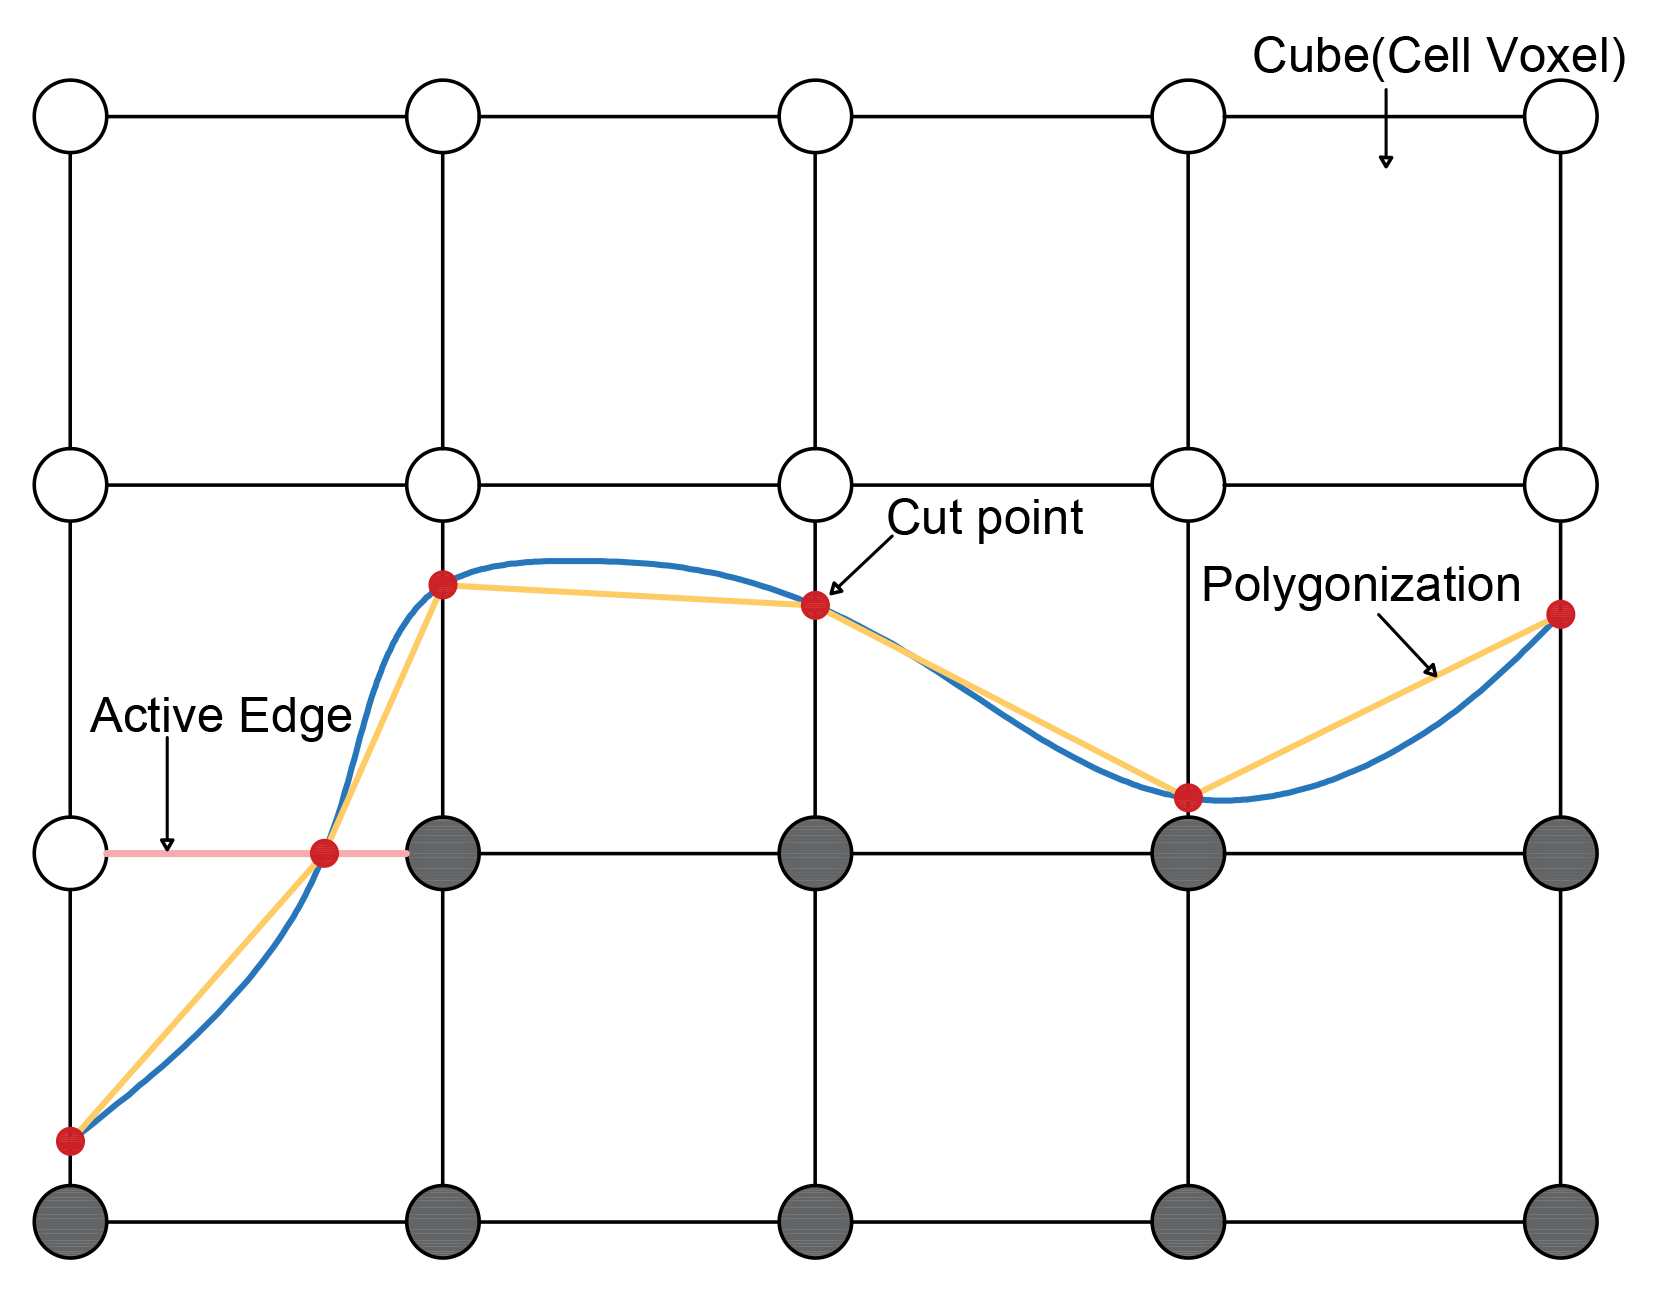
\includegraphics[height=0.5\textwidth,width=0.6\textwidth]{Figures/Regular_grid.jpg}
    \decoRule
    \caption{Regular grid}
    \label{fig:Regular-grid}
    \end{figure}
    
    \item \textbf{Unstructured Grid:} This is a grid where the cells can have arbitrary shapes and sizes. This grid type is often used for complex geometries or when the data is irregularly sampled.
    \vspace{1.5mm}

    \item \textbf{Adaptive Grid:} This is a grid where the cell size can vary across the space. This grid type is often used to represent spaces where the data has varying levels of detail or complexity. Octrees and quadtrees are types of adaptive grids. Fig. \ref{fig:quadtree} illustrates a quadtree, a tree data structure in which each internal node has exactly four children. An octree is the three-dimensional version of this structure, where each internal node has eight children, one for each octant of the 3D space.

    \begin{figure}
    \centering
    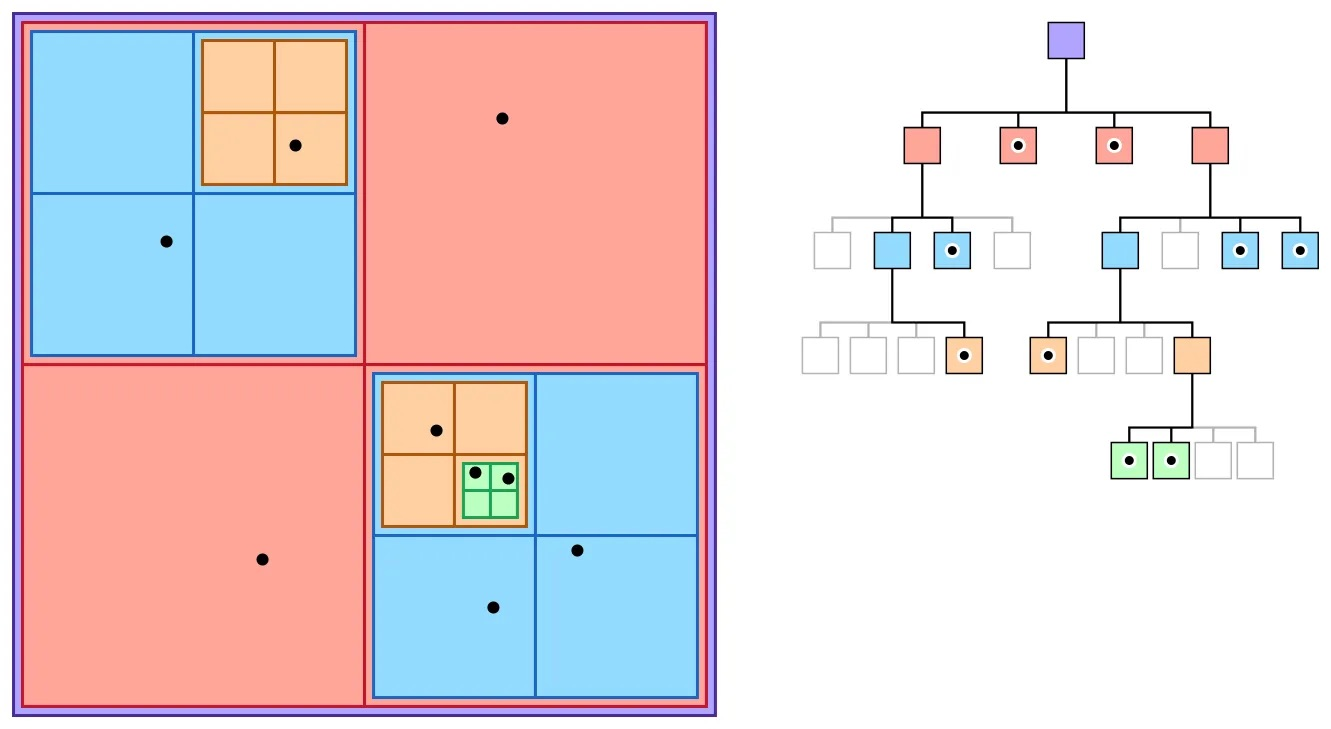
\includegraphics[height=0.45\textwidth,width=0.87\textwidth]{Figures/quadtree.jpeg}
    \decoRule
    \caption{Representation of quadtree}(\cite{image_quadtree})
    \label{fig:quadtree}
    \end{figure}
    
    \vspace{1.5mm}
    \item \textbf{Irregular Grid:} This is a grid where the cells can have different shapes and sizes. An unstructured grid is a type of irregular grid.
    \vspace{1.5mm}
    \item \textbf{Active Edge:} An edge of a grid cell intersected by the isosurface. The isosurface passes through the active edges of the grid.
    \vspace{1.5mm}
    \item \textbf{Isosurface:} An isosurface is a three-dimensional surface representing points of a constant value (or isovalue) within a volume of space. This volume of space is often represented as a 3D scalar field, which is a function that assigns a scalar value like density, temperature, and pressure to every point in a 3D space.
    \vspace{1.5mm}
    \item \textbf{Isovalue:} The isovalue is the specific value used to extract the isosurface from the 3D scalar field. For example, an isosurface might be extracted from a 3D Computed Tomography (CT) scan or Magnetic Resonance Imaging (MRI) at an isovalue representing bone density in medical imaging. This would result in a 3D surface representing the bones' or internal organ's boundary within the body. Figure \ref{fig:isovalue} shows the cross-section of a smooth sphere and its isosurface, marked with red, at two different isovalues, namely 50 and 200.
    
    % \begin{figure}
    % \centering
    % \includegraphics[width=\textwidth]{Figures/isovalue.png}
    % \decoRule
    % \caption{TO BE DELETED Multiple quad-trees (2D octrees) as \textbf{a} unstructured and \textbf{b} structured topologies}(\cite{image_quadtree_structured_unstructured})
    % \label{fig:types-of-grid-deleted}
    % \end{figure}

    \begin{figure}
    \centering
    \includegraphics[width=1.0\textwidth]{Figures/isovalue.jpg}
    \decoRule
    \caption{Cross-section of a smooth sphere (left), and surface marked with red iso-value set to 50 (middle) and iso-value set to 200 (right)}(\cite{image_quadtree_structured_unstructured})
    \label{fig:isovalue}
    \end{figure}
    
    \vspace{1.5mm}
    \item \textbf{Polygonization of isosurfaces:} The process of approximating isosurfaces using polygons, typically triangles, to create a mesh representing the surface in a 3D scalar field.
\end{itemize}


\section{Hermite Data} \label{Section 2.2}
Compared to scalar fields alone, Hermite data is a complex data format that provides a greater understanding of the underlying geometry. It encompasses derivatives at discrete places in space and scalar values (\cite{Hammarstrom_2013}). Hermite data offers a more thorough representation of geometric properties, including curvature, gradients, and shape changes, by including directional information through derivatives. In scientific and technical fields, this enhanced representation has proven essential for capturing complex structures and enabling more precise assessments (\cite{Markiewicz_Koperwas_2021}).

\paragraph{Challenges in Meshing Hermite Data:}
\begin{itemize}
    \item \textbf{Non-Uniform Data Distribution:} A non-uniform distribution of sample points within the spatial domain is a common feature of Hermite data. Variations in the local feature density or sample preferences cause this non-uniformity (\cite{Hammarstrom_2013}).
    \item \textbf{Varying Levels of Smoothness:} Derivatives of Hermite data reveal details on regional differences in smoothness. While some data areas may be smooth, others may have sudden shifts or discontinuities (\cite{Dai_2007}).
    \item \textbf{Discontinuities and Sharp Features:} Sharp edges, corners, and other geometric discontinuities can be represented via Hermite data. However, certain methods are needed to capture these properties correctly in a mesh (\cite{Hammarstrom_2013}).
    \item \textbf{Local Adaptation to Hermite Data:} The geometric diversity of Hermite data necessitates meshing methods that can dynamically adjust to changes in curvature and form. The tiny features and subtle fluctuations found in the data may be difficult to capture using conventional techniques that are not designed for Hermite data (\cite{Dai_2007}).
\end{itemize}

\section{Conformal Meshing and Geometric Accuracy} \label{Section 2.3}
Within computer graphics and scientific visualization, conformal meshing is seen as a crucial tenet, a passageway for depicting complicated real-world objects and data into coherent visual representations that may also be useful from an analytical standpoint. The fundamental skill of conformal meshing is the smooth transformation of complex geometric properties, such as curvature, sharp edges, corners, and other delicate subtleties, from the abstract world of data into concrete, detectable structures (\cite{Benkler_2008}). This process is the basis for accurate physical modeling, realistic visual simulations, and scientific comprehension across various fields. The core of conformality is the capacity to guarantee that the mesh, the discrete digital counterpart of the continuous physical environment, stays an accurate reflection of the underlying data. Contrary to traditional meshing techniques, which could unintentionally blur fine details or alter geometrical characteristics, conformal meshes accurately reflect the data's complexity. Viewers or analysts are given access to a more accurate picture of the actual item or phenomena when interacting with these meshes, offering insights that would not otherwise be possible (\cite{Dai_2007}).

The maintenance of geometric correctness is at the core of conformal meshing. Geometric correctness refers to how accurately the mesh represents the complex geometrical characteristics of underlying data, ensuring that critical details like forms, angles, and proportions are preserved in the meshed representation. This level of precision is especially crucial when working with complicated objects with various degrees of curvature or sharp features since any divergence from the original geometry might result in misleading representations or incorrect assessments (\cite{Benkler_2008}). Think about a scenario where fluid flow simulations are performed across the surface of an airplane wing. To accurately forecast aerodynamic behaviors, the complex curvature of the wing, including regions of high curvature near edges and corners, must be accurately represented. A solid modeling foundation built on a conformal mesh that correctly preserves these geometric details yields more precise insights into lift, drag, and other aerodynamic phenomena. Similarly, conformal meshing in medical imaging ensures anatomical features are correctly represented, enabling precise analysis for surgery planning or disease diagnosis (\cite{Chen_2022}). 
However, conformal meshing presents several difficulties in obtaining geometric precision. It necessitates overcoming the technical obstacles of discretization, interpolation, and error correction. The subtleties of data encoding, such as Hermite data, add smoothness variations and possibly discontinuities to the complexity (\cite{Chen_2022}). In order to address these nuances, meshing algorithms need to maintain topological consistency and integrity. Often, solving these problems requires striking a delicate balance between computational accuracy and efficiency. To achieve this balance, sophisticated algorithms and optimization techniques are used, guaranteeing that the resultant conformal meshes are accurate representations of the underlying data and suitable for simulations and real-time display. The quest for geometric correctness within conformal meshing is a dynamic and expanding frontier, necessitating interdisciplinary collaboration and novel strategies as the demands for increasingly elaborate and accurate representations increase (\cite{Benkler_2008}).

\subsection{Challenges in Achieving Conformal Meshing}
A key component of computer graphics and scientific visualization, conformal meshing offers the potential to convert complex data into accurate and aesthetically pleasing representations. However, there are obstacles to overcome in order to achieve geometric precision in conformal meshing (\cite{Dai_2007}). 
\begin{itemize}
    \item \textbf{Dissecting Complexity:} In conformal meshing, complexity may refer to various things, including the fine geometric details of objects and the depth of data representation. Sharp edges, subtle changes in curvature, and complicated surface patterns are just a few examples of the many characteristics that real-world objects frequently display. To capture these details, a mesh must be carefully resolved to retain a degree of geometric precision that accurately depicts the object's original shape. The difficulty comes from balancing the many smoothness levels, probable discontinuities, and uneven data distribution in Hermite data. Therefore, conformal meshing for Hermite data requires methods to deal with these difficulties while maintaining geometric precision and topological consistency (\cite{Chen_2022}).
    \item \textbf{The Efficiency Conundrum:} While pursuing geometric correctness is crucial, computing efficiency cannot be sacrificed, especially when real-time interactions or extensive simulations are required. The generation and rendering of high-resolution conformal models, which faithfully represent subtle geometric features, can be computationally taxing. Therefore, the difficulty is in effectively converting complicated data into meshes that balance complexity and processing expense (\cite{Alexa_2009}).
    \item \textbf{Strategies for Balancing Complexity and Efficiency:} Conscientiously employing techniques that use computational innovation and subject-matter expertise is necessary to balance complexity and efficiency in conformal meshing (\cite{Zhang_2012}). Utilizing adaptive mesh refinement, a method that dynamically modifies the mesh resolution based on the local properties of the data is one strategy. Because of this, regions with complex geometries can have better resolution, whereas smoother parts can use coarser components. Adaptive refinement maximizes geometric accuracy and computing economy by concentrating computational resources where they are most helpful. The effectiveness of conformal meshing can be improved by creating customized algorithms that use the built-in structure of the data (\cite{Markiewicz_Koperwas_2021}).
\end{itemize}



\section{Modeling Object Surfaces through Surface Extraction} \label{Section 2.4}
Surface extraction is a pivotal technique in computational geometry and computer graphics, bridging raw data representation and a structured geometric model. By extracting the surface from a set of data points or a volumetric representation, one can obtain a mesh or a set of primitives that closely approximates the original object's shape. This is particularly useful in applications like medical imaging, where accurate representation of organ surfaces can aid in diagnostics and surgical planning (\cite{Lorensen_1987}).

The process often involves techniques like the Marching Cubes (MC) algorithm, which is elaborated upon in Section \ref{Marching-Cubes}, that converts volumetric data into a triangulated mesh. This mesh can then be refined, smoothed, or further processed to achieve the desired level of detail and accuracy (\cite{Newman_2006}).

Once the surface is extracted, it serves as a foundational representation for various computational and graphical tasks. This structured geometric model enables more efficient computations, especially in rendering techniques like ray tracing. By accurately modeling an object's surface, we can achieve more realistic and precise visualizations, highlighting the critical role of surface extraction in the broader context of computer graphics and simulation (\cite{Whitted_1980}).

\section{Ray Tracing in Surface Extraction} \label{Section 2.5}
Ray tracing is an essential technique in computer graphics to mimic light behavior and, ideally, produce incredibly realistic visuals (\cite{Glassner_1989}). Finding the color and intensity of each pixel in the final picture requires tracking the movement of light beams as they interact with scene elements. This method accounts for the complex interactions between light and diverse surfaces, including reflection, refraction, and shadow casting (\cite{Parker_1999}).
Ray tracing excels in displaying isosurfaces in volumetric data, for example. Volumetric data, such as those from X-rays or scientific simulations, are three-dimensional data that define a volume's characteristics. The surfaces inside a volume with a constant value, such as a specific density or temperature, are known as isosurfaces (\cite{Aaron_2007}).

Ray tracing makes it possible to faithfully portray the intricate light interactions in volumetric data, producing very realistic and eye-catching renderings of isosurfaces (\cite{Glassner_1989}). The realism and depth of the produced pictures are improved by the accuracy of ray tracing in capturing minute fluctuations in lighting and shading. This skill is priceless in areas such as medical imaging, scientific visualization, and computer-aided design, where precise surface extraction and volumetric data visualization are essential for analysis and comprehension (\cite{Parker_1999}).

\subsection{Basics of Ray Tracing} 
The ray-tracing algorithm builds an image by extending rays into a scene and bouncing them off surfaces and toward sources of light to approximate the color value of pixels.
The computer graphics method of ray tracing models the behavior of light in a virtual scene. It starts by casting light onto the scene from the spectator's viewpoint (\cite{Haines_Akenine_2019}). As they go around the virtual world, these rays interact with the surfaces they come across. They replicate several optical effects dependent on the characteristics of those surfaces when they encounter objects, including reflection, refraction, and shadowing. The essential idea behind ray tracing is to identify the color of each pixel in a picture by examining the light that comes from the direction that corresponds to that pixel and hits the viewer's eye. This procedure entails following each ray's passage from the viewer's eye into the picture backward and analyzing the interactions it encounters (\cite{Haines_Akenine_2019}). As illustrated in Fig. \ref{fig:ray_casting}, The ray-tracing algorithm builds an image by extending rays into a scene and bouncing them off surfaces and toward light sources to approximate the pixels' color value.

\begin{figure}
    \centering
    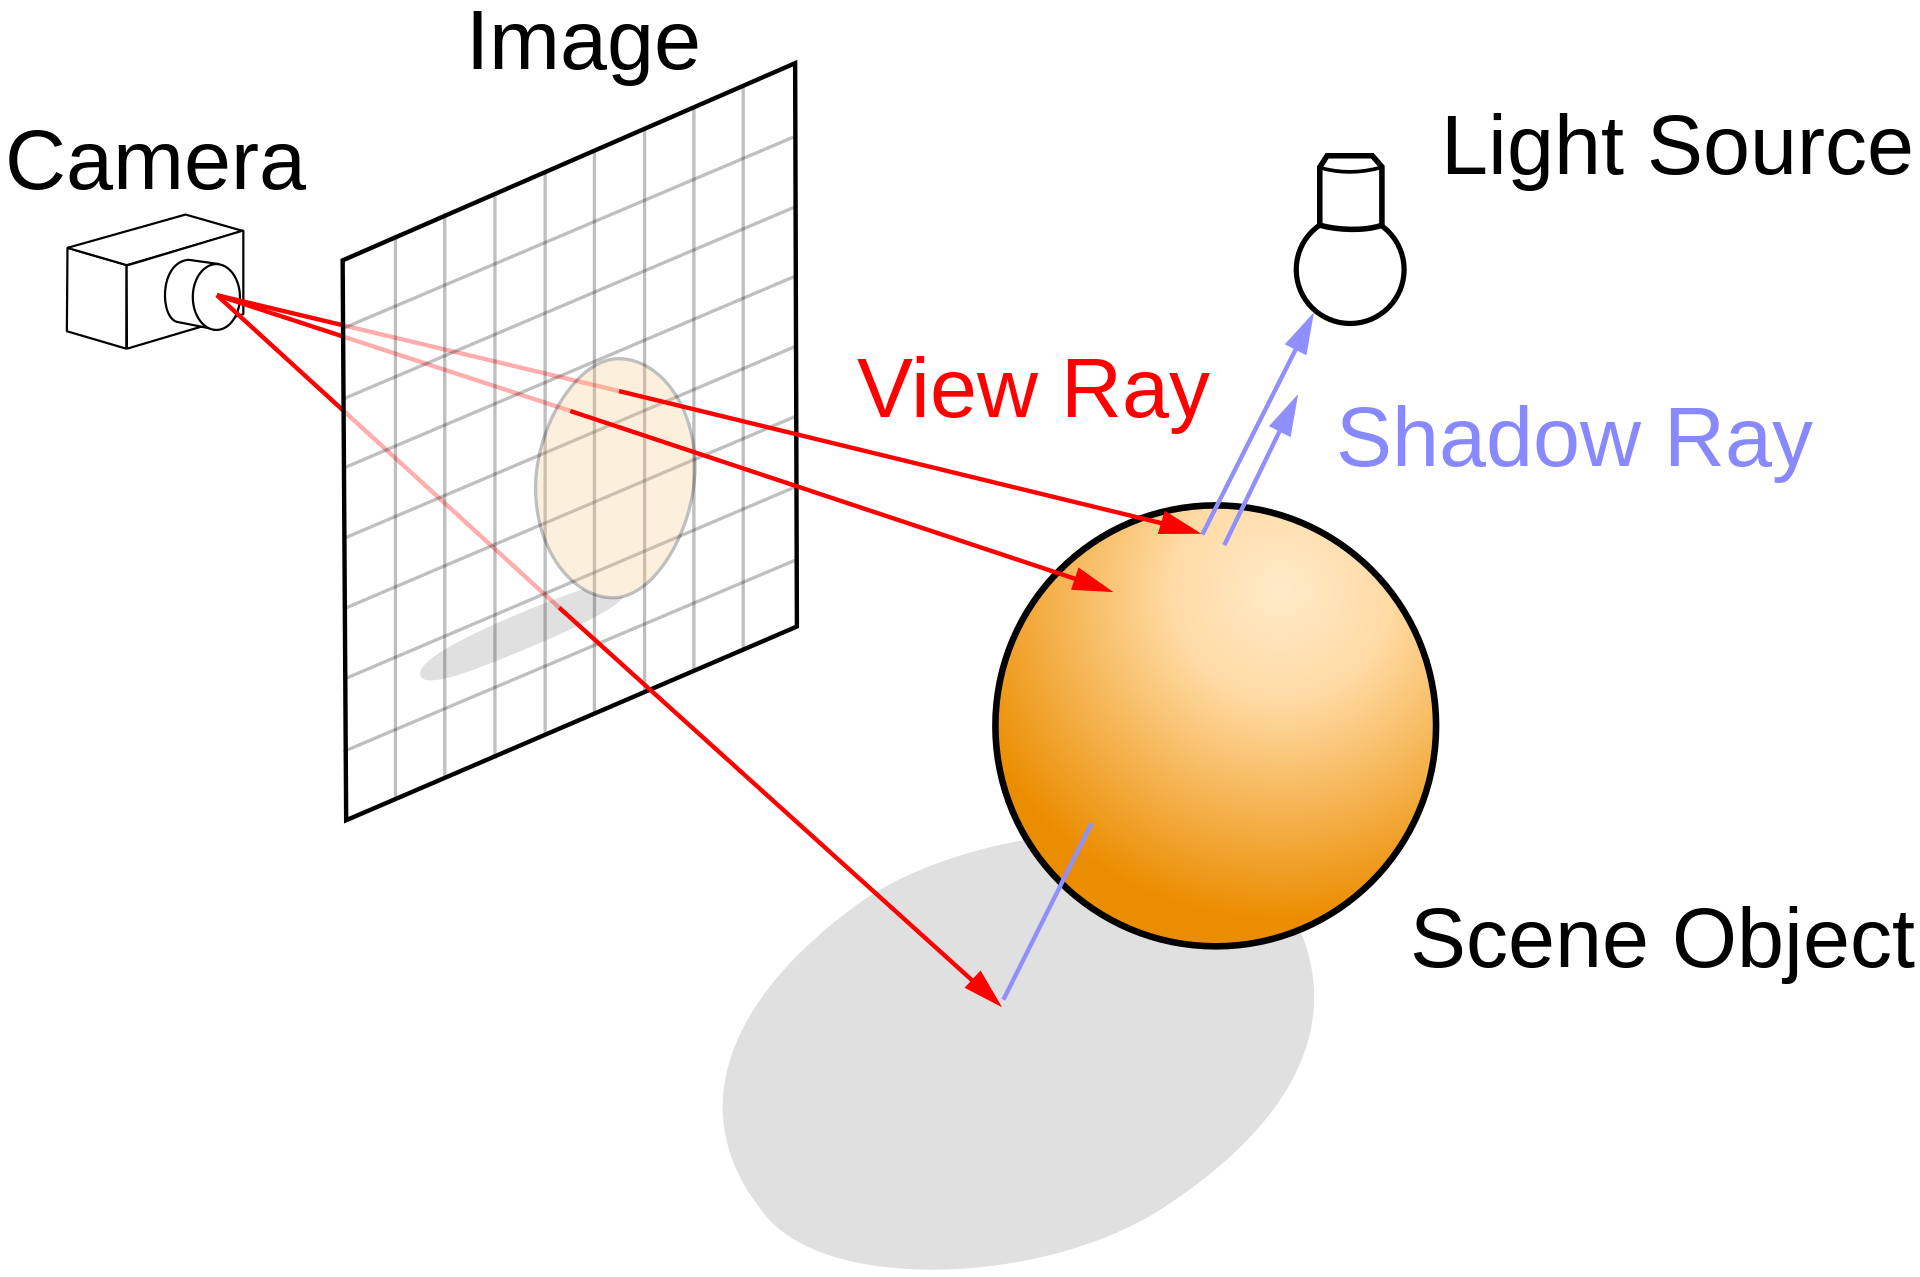
\includegraphics[height=0.4\textwidth,width=0.55\textwidth]{Figures/Ray_trace_diagram.png}
    \decoRule
    \caption{Ray tracing}(\cite{image_raytracingimage})
    \label{fig:ray_casting}
\end{figure}

Ray tracing permits the development of very realistic pictures by considering elements like the material qualities of surfaces, the angle of incidence, and the dispersion of light sources (\cite{Haines_Akenine_2019}). When objects partly obstruct light, they may capture subtle effects like soft shadows, which provide seamless transitions between lighted and shadowed parts. In order to replicate phenomena like depth of field, which causes objects to look in or out of focus depending on their proximity to the observer, ray tracing is also used. Additionally, it can mimic global illumination, considering indirect lighting and how light interacts with various surfaces in a scene and bounces off of them. Ray tracing has been a critical computer graphics technology since it was first used by \cite{Glassner_1989}, and it has continued to advance to produce generated pictures with higher degrees of photorealism (\cite{Haines_Akenine_2019}).

\subsection{Importance of Ray Tracing in Isosurface Extraction} 
Ray tracing, a cornerstone technique in computer graphics, is renowned for its ability to simulate intricate light interactions, producing highly realistic visuals. While it's often associated with rendering effects like shadows and transparency (\cite{Parker_1999}), the core functionality of ray tracing is pivotal for the specific application discussed in this work: surface point detection and the subsequent calculation of the Quadratic Error Function.

In the context of our research, ray tracing is employed not for its visual rendering capabilities but for its precision in detecting intersections. By firing a ray along each mesh line, we can accurately determine the point at which the ray intersects the surface. This intersection, or "hit point," along with the normal to that point, becomes instrumental in our calculations.

By accurately visualizing and analyzing complex structures and occurrences, integrating isosurface extraction with ray tracing helps researchers and scientists better interpret volumetric data. Precisely depiction of isosurfaces is crucial for efficient data processing and interpretation in various sectors, including engineering, scientific visualization, and medical imaging (\cite{Dai_2021}).

\subsection{Overview of Intel Embree API} \label{Intel-Embree-Overview}
Ray-tracing kernels with strength and speed are available via the Intel Embree API (\cite{Sato_2021}). It provides highly optimized methods for quickly computing ray-primitive crossings and is mainly created to use contemporary CPU architectures' capabilities. Embree is an excellent option for computationally demanding applications like isosurface extraction because the accuracy of ray tracing computations is essential. Embree may be easily integrated into various applications because of its modular design. Developers may use Embree's optimized ray tracing capabilities, assuring quick and precise calculations, by smoothly integrating Embree into their applications. The API offers adaptable and effective methods that let programmers use ray tracing on CPUs (\cite{Ingo_2014}).
Embree's capability to handle dynamic scenarios with ease is a noteworthy feature. As a result, Embree enables real-time interactions and dynamic visualizations in situations where the scene geometry varies over time. Embree is a popular option because of its capabilities for applications like interactive simulations, virtual reality, and gaming that need immediate response and fluid visualization. Developers may use Embree to create high-performance calculations and realistic visualizations using its optimized ray-tracing kernels. The API is an invaluable resource for various applications that need both speed and precision in ray tracing operations due to its emphasis on practical ray-primitive intersection computations, its modular design, and its support for dynamic scenes (\cite{Sato_2021}).

While the Intel Embree API is primarily designed for optimized ray tracing on CPUs, it is worth noting that the API also supports hardware-accelerated ray tracing on Intel GPUs through the SYCL programming language. This GPU support can significantly enhance the performance of ray tracing applications, especially when real-time graphics are a priority.

However, the CPU remains a more suitable choice for applications that do not demand real-time processing. Here are some reasons why the CPU version of the Intel Embree API is preferable:

\begin{itemize}
    \item \textbf{Maturity and Testing}: The CPU version of Embree is more mature and has undergone extensive testing, ensuring reliability and stability.
    \item \textbf{Wider Support}: It is more widely supported, allowing integration with a broader range of applications.
    \item \textbf{Ease of Use}: The CPU version is more straightforward to learn and implement. Unlike the GPU version, it does not necessitate expertise in GPU programming paradigms.
\end{itemize}

In summary, while the Intel Embree API offers enhanced performance on GPUs, its CPU-focused design is particularly advantageous for tasks, prioritizing accuracy, computational intensity, and ease of use over real-time responsiveness.

\section{Challenges in surface Extraction} \label{Section 2.6}
A strong method for analyzing and visualizing 3D scalar fields is surface extraction. However, the nature of the data, techniques, and expected results provide several difficulties.
\subsection{Data Resolution and Quality}
The resolution of a dataset dramatically influences the quality and detail of the extracted surface during isosurface extraction. Surfaces that are simplistic and devoid of finer features may be produced by low-resolution data when sample points are sparser. This might reduce the accuracy and realism of the extracted surface by causing the loss of crucial details and features in the visualization (\cite{Knoll_2021}).

On the other hand, high-resolution data captures a larger number of sample points, enabling a more accurate representation of the underlying scalar field (\cite{Knoll_2021}). Surfaces with minute features and slight data variances are produced as a consequence. High-resolution data processing, however, may be computationally costly. The growing amount of data points needs additional computing capacity and processing power to execute the required computations. Longer processing times may result, particularly in complicated or real-time systems where prompt feedback and interactive features are essential (\cite{Knoll_2021}).

Therefore, it is crucial to balance computing efficiency and resolution. It entails choosing a resolution that will capture the necessary degree of detail while considering the application's performance needs and the available computing resources. This compromise makes the extracted surface accurate and aesthetically pleasing without compromising performance or real-time responsiveness (\cite{Knoll_2021}).

\subsection{Noise and Artifacts}
Noise is a typical feature of real-world datasets, which may harm the precision and quality of the retrieved surface during isosurface extraction. Noise is the term for arbitrary or undesirable oscillations in the data that do not accurately represent the underlying scalar field's genuine characteristics. These variations may be caused by many things, including measurement blunders, sensor noise, or built-in constraints in data-collecting procedures (\cite{Savchenko_1995}).
To ensure the fidelity of the extracted surface, it is imperative to address these challenges. While there are techniques to mitigate noise, they might inadvertently suppress genuine data features. Similarly, rectifying artifacts without domain-specific knowledge can be challenging. The overarching challenge is to discern and address noise and artifacts without compromising the integrity of the actual data features.

\subsection{Computational Overhead}
Extracting surfaces from big datasets may be computationally taxing for real-time or interactive applications. The computational burden of surface extraction rises as datasets are more extensive and complicated. Optimized algorithms and effective data structures are required to minimize processing time and memory utilization to handle this. These methods seek to accelerate surface extraction, allowing quick calculations and responsive user interfaces even for complex and large datasets (\cite{Lewiner_2003}).

\subsection{Ambiguities in Scalar Fields}
During the surface extraction process in scalar fields, locations where the values vary quickly create a problem. One of the primary issues is the ambiguity that arises when determining the topology of the isosurface in regions where the scalar field values are close to the isovalue.

Several solutions have been proposed to address these ambiguities. \cite{Nielson_1991} introduced the "asymptotic decider" to resolve the ambiguity based on the local behavior of the scalar field.

Despite these advancements, ambiguities in scalar fields still need to be solved, requiring careful consideration to ensure accurate and topologically correct surface extraction.

\subsection{Hardware and Software Limitations}
The limits of the hardware and software platforms in use also impact how effective surface extraction is. Powerful hardware is often needed to handle modern datasets promptly. Software solutions must also be tailored to their particular hardware, using parallel processing strategies, GPU acceleration, and other cutting-edge computing approaches.

\section{Summary}
In this chapter, we delved deep into the intricacies of surface extraction, emphasizing its significance in various domains like computer graphics, scientific visualization, and medical imaging. We started by understanding the foundational role of meshes in representing continuous domains and the challenges posed by data-driven representations like Hermite data. The glossary section provided a comprehensive overview of the technical terms, ensuring clarity in the subsequent discussions.

We then explored the nuanced challenges posed by Hermite data in meshing, emphasizing the non-uniform distribution, varying levels of smoothness, and the presence of discontinuities. The discussion on conformal meshing highlighted the importance of geometric accuracy in representing real-world objects and the challenges in achieving it. The balance between computational accuracy and efficiency was underscored, emphasizing the need for innovative algorithms and optimization techniques.

The section on surface extraction provided insights into the process of converting volumetric data into structured geometric models, with ray tracing playing a pivotal role in achieving realistic visualizations. The challenges in surface extraction, ranging from data resolution to ambiguities in scalar fields, were discussed in detail, highlighting the complexities involved in the process.

This chapter provided a comprehensive overview of the complexities and nuances associated with meshing and surface extraction. As we move forward, these foundational concepts will serve as a backdrop for more in-depth discussions on specific algorithms and techniques in the realm of isosurface extraction.
\chapter{Literature Review}  \label{Chapter3} 
This chapter delves into the extensive literature surrounding isosurface extraction techniques. Isosurface extraction is pivotal in computer graphics, medical imaging, geophysics, and scientific visualization. The objective is to transform volumetric data into a visual representation, allowing a more intuitive understanding of the underlying information. Over the years, numerous algorithms and methodologies have been proposed, each with unique advantages and challenges. This chapter aims to comprehensively review these methods, focusing on their principles, algorithms, advantages, limitations, and applications. By the end of this chapter, readers should have a holistic understanding of the evolution and current state of isosurface extraction and mesh generation techniques.

\section{Marching Squares} \label{Marching-Squares}

Marching Squares (MS) is a contouring technique primarily used for 2D scalar fields. It is the 2D counterpart to the Marching Cubes algorithm (explained in detail in \ref{Marching-Cubes}), which operates in three dimensions. Marching Squares is primarily designed to derive contour lines, also known as isolines, from two-dimensional scalar fields. This technique is invaluable in various applications, ranging from creating topographic maps that represent terrain elevations to detecting contours in images, aiding in image analysis. By interpreting and visualizing data gradients, Marching Squares provides a clearer understanding of spatial variations and patterns, making it an essential tool in geospatial analysis, computer graphics, and digital image processing (\cite{Maple_2003}).

\vspace{2mm}
\subsection{Basic Principle}

The Marching Squares algorithm operates by dividing the 2D scalar field into a grid of squares. Each corner of these squares (or cells) is sampled to determine its scalar value. Based on these values, a specific configuration for the square is determined, which dictates how the contour line will pass through the square. Lookup tables are then employed to triangulate the square based on its configuration, resulting in a segment of the contour line.

\vspace{2mm}
\subsection{Algorithm Overview}

\begin{itemize}
\item \textbf{Grid Formation:} The 2D scalar field is divided into a grid of squares.

\item \textbf{Corner Sampling:} The scalar value at each corner of the square is determined, as denoted in Fig \ref{fig:Marching-Square-cell}.

\begin{figure}[H]
\centering
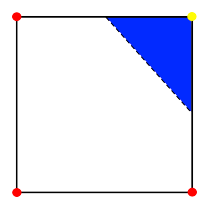
\includegraphics[height=0.3\textwidth,width=0.3\textwidth]{Figures/Marching-Sqaure-cell.png}
\decoRule
\caption{A marching square. The points at the corners denote the
sample points. Red points are outside the isoline and yellow point is inside the isoline. The dotted line marks the isoline, and the blue color defines the ’inside’} (\cite{Rassovsky_2014})
\label{fig:Marching-Square-cell}
\end{figure}

\item \textbf{Configuration Determination:} The four corners of each square provide \(2^4 = 16\) possible configurations, as displayed in Fig \ref{fig:Marching-Square-lookup-table}. With rotational and reflective symmetry, all possible combinations were reduced to 4 distinct configurations (Fig. \ref{fig:MS-4-unique-case}). A configuration for the square is identified Based on the scalar values at the corners and a specified isovalue.

\begin{figure}
\centering
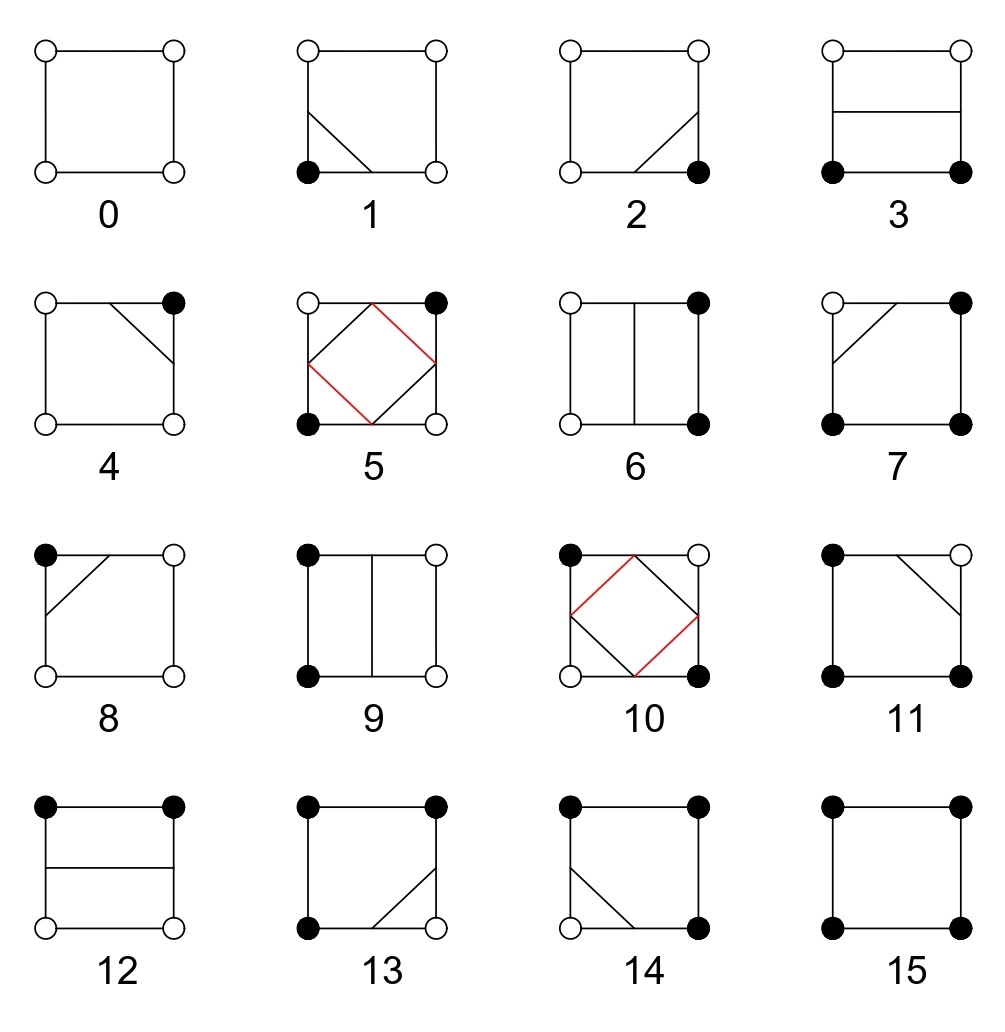
\includegraphics[width=0.85\textwidth]{Figures/Marching-Square-lookup-table.jpg}
\decoRule
\caption{The Marching Squares algorithm presents 16 configurations, with ambiguous scenarios evident in cases 5 and 10, highlighted by red lines.} (\cite{Rassovsky_2014})
\label{fig:Marching-Square-lookup-table}
\end{figure}

\begin{figure}
\centering
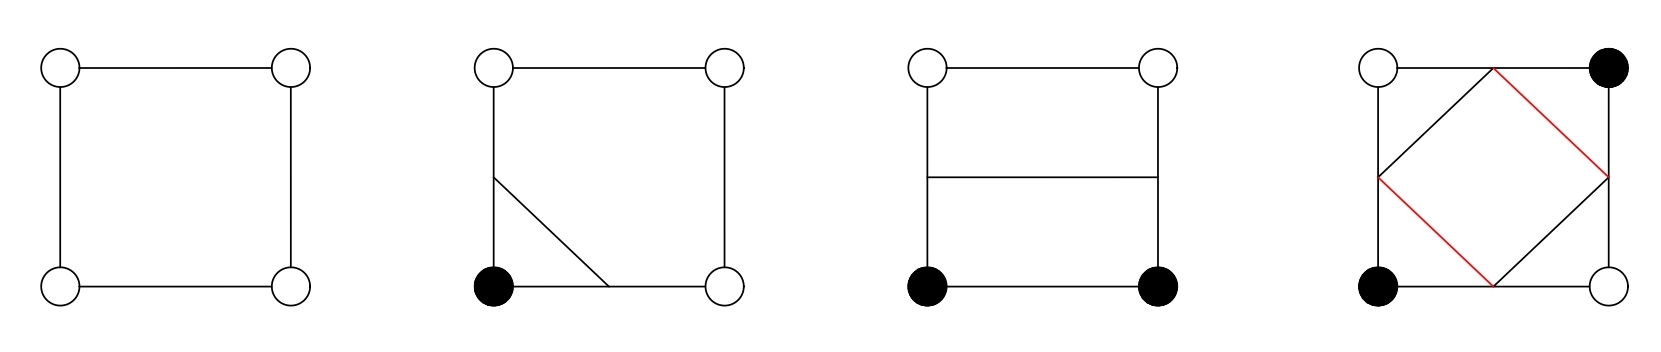
\includegraphics[width=0.90\textwidth]{Figures/MS-4-unique-case.jpg}
\decoRule
\caption{The 4 unique configurations of the Marching Squares algorithm, which are necessary to reproduce all others.} (\cite{Rassovsky_2014})
\label{fig:MS-4-unique-case}
\end{figure}

\item \textbf{Lookup Tables:} Using the determined configuration, lookup tables provide the necessary information to triangulate the square and extract the contour segment.

\item \textbf{Contour Construction:} The contour segments from each square are combined to form the complete contour line for the scalar field.
\end{itemize}

\subsection{Applications}

\begin{itemize}
\item \textbf{Robotic Manipulation:}
The fast marching square method, a variant of Marching Squares, has been employed in kinesthetic learning for robotic manipulation, allowing robots to learn from human demonstrations and adapt to their environment (\cite{Prados_2023}).

\item \textbf{Feature Preservation in 3D:}
The Marching Squares principle has been extended to 3D scenarios, as seen in the Cubical Marching Squares (CMS) algorithm, which aims to preserve sharp features in volumetric data (\cite{Chien-Chang_2005}).

\item \textbf{Topographic Mapping:} The algorithm is widely used in generating topographic maps, where contour lines represent constant elevation levels.

\item \textbf{Image Processing:}
Marching Squares can be used for image contour detection, aiding in object recognition and other image analysis tasks.
\end{itemize}

\subsection{Advantages}
\begin{itemize}
\item \textbf{Simplicity}: The algorithm is relatively straightforward to implement, especially compared to its 3D counterpart, Marching Cubes.
\item \textbf{Efficiency}: Marching Squares can quickly generate contour lines for large 2D scalar fields.
\end{itemize}

\subsection{Limitations}
\begin{itemize}
\item \textbf{Ambiguities}: When considering the problem in MS, there are two configurations, which could result in ambiguous topology. That is to say, the decision of which case should be used is undefined by the algorithm. Those cases, for the MS algorithm, are visible in Fig \ref{fig:ambiguity}.

\begin{figure}[H]
\centering
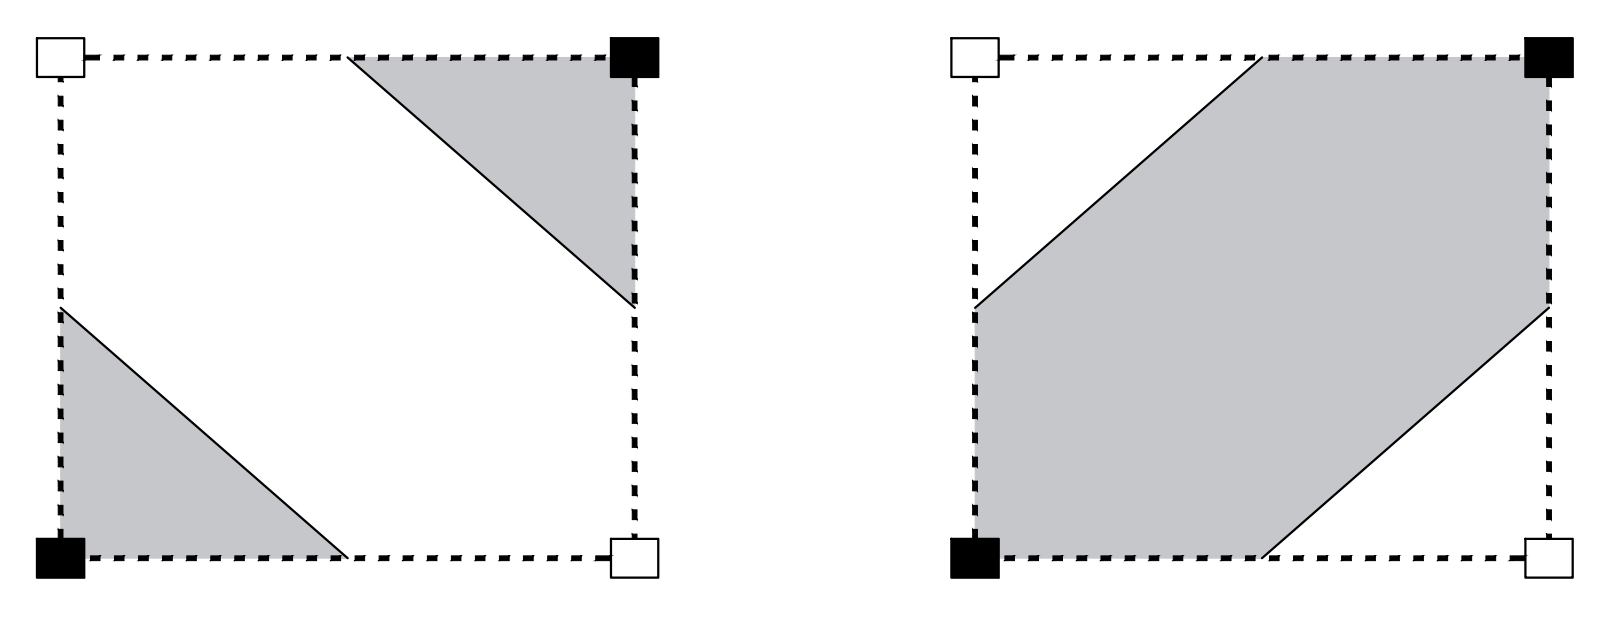
\includegraphics[height=0.26\textwidth,width=0.55\textwidth]{Figures/ambiguity.jpg}
\decoRule
\caption{The black corners are inside the surface. For this specific case, there are two possible configurations. This is then considered a face ambiguity.} (\cite{Chien-Chang_2005})
\label{fig:ambiguity}
\end{figure}

\item \textbf{Resolution Dependency}: The quality and accuracy of the extracted contour lines can be highly dependent on the resolution of the grid.
\end{itemize}

\section{Marching Cubes} \label{Marching-Cubes}

A crucial computer graphics method called Marching Cubes (MC) was created in 1987 by \cite{Lorensen_1987}. It is intended to produce a polygonal mesh representing an isosurface inside a 3D grid of data points and is often used in industries including geophysics, scientific visualization, and medical imaging. MC revolutionized these fields by transforming challenging scalar field data into intuitive 3D representations. It is necessary for portraying complicated structures, allowing scientists and medical practitioners to visualize and analyze data more comprehensibly and educationally, eventually improving diagnostic and research capacities and furthering our knowledge of complex phenomena (\cite{Lorensen_1987}).

\vspace{2mm}
\subsection{Basic Principle}

The fundamental concept of MC is to subdivide a 3D scalar field into a collection of tiny cubes, provided that a regular grid represents the field. The method selects the polygon(s) that correspond to the portion of the isosurface that traverses each cube.

\vspace{2mm}
\subsection{Algorithm Overview}

\begin{itemize}
\item \textbf{Cube classification:} Cube classification classifies a three-dimensional cube's interior according to the values assigned to each of its eight corners. 
Each corner may have a value that is either higher or lower than the isovalue, which leads to 256 different configurations. With rotational and reflective symmetry authors (\cite{Lorensen_1987}) reduced all possible combinations to these to 15 distinct configurations (Fig. \ref{fig:MC-15-cases}), making it easier to analyze and describe intricate 3D data structures.

\begin{figure}
\centering
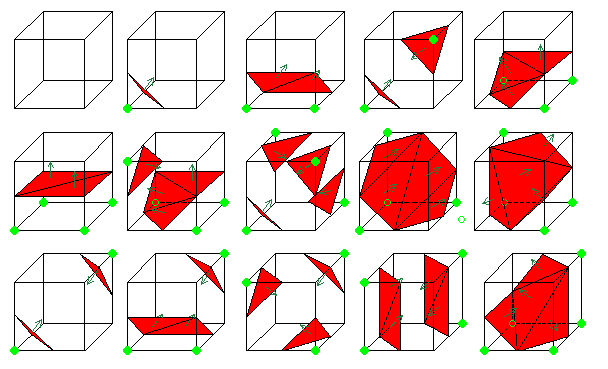
\includegraphics[height=0.6\textwidth,width=0.9\textwidth]{Figures/MC-15-cases.png}
\decoRule
\caption{Illustration of the 15 configurations of the marching cubes technique. The green vertices are the ones classified as “inside” the isosurfaces, whereas the remaining ones as “outside”.} (\cite{Lorensen_1987})
\label{fig:MC-15-cases}
\end{figure}
    

\item \textbf{Edge Intersection:}
The Marching Cubes algorithm works by dividing the volumetric dataset into small cubes. For each cube, the algorithm determines where the isosurface intersects the cube's edges. This is done by checking the scalar values at the cube's vertices against the isosurface's value. If one vertex is below the isosurface value and the other is above, the edge is intersected by the isosurface. The exact location of the intersection can be determined using linear interpolation between the two vertex values (\cite{Lorensen_1987}).
\item \textbf{Polygon Construction:}
Once the intersections are identified, the next step is constructing polygons that approximate the isosurface within the cube. This is typically done using a precomputed table, known as the edge or triangle table. This table provides a lookup for connecting the intersections based on the specific scalar values at the cube's vertices. The result is a set of triangles that approximate the isosurface within the cube (\cite{Lorensen_1987}).
\item \textbf{Mesh Generation:}
The ultimate 3D mesh representation of the isosurface is created during the "Mesh Generation" step of isosurface extraction. This stage merges the polygons produced from each cube in the volumetric dataset.  The mesh quality depends on the edge intersection calculations' accuracy and the polygons' correct construction. Once the mesh has been created, it may be displayed and altered for various uses, including computer graphics, medical imaging, and scientific visualization, giving essential insights into the underlying data (\cite{Wilhelms_1990}).
\end{itemize}

\subsection{Advantages}
\begin{itemize}
\item \textbf{Efficiency:} MC is relatively fast and can be applied to run in real-time for specific applications.
\item \textbf{Simplicity:} The algorithm is theoretically straightforward and relies on lookup tables for operation.
\end{itemize}

\subsection{Limitations} 
\begin{itemize}
\item \textbf{Ambiguities and Topological Errors:}
One of the most significant issues with the innovative Marching Cubes algorithm is the presence of unclear cases (Fig. \ref{fig:MC-ambiguity}). These ambiguities arise when the isosurface intersects the cube in a way that there are multiple conceivable ways to triangulate the intersected boundaries, leading to different topologies (\cite{Nielson_1991}).

\begin{figure}
\centering
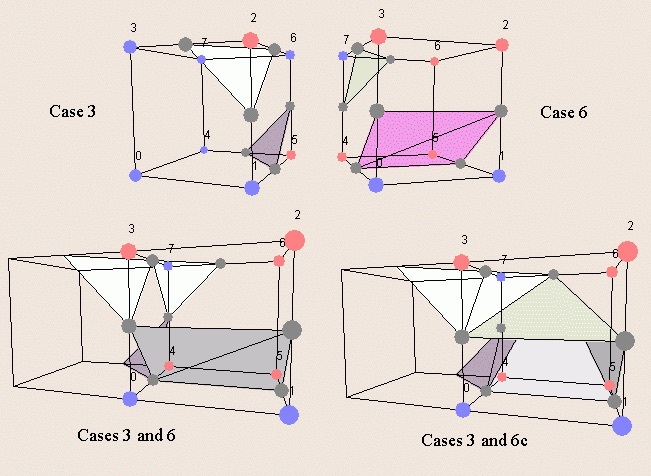
\includegraphics[height=0.55\textwidth,width=0.88\textwidth]{Figures/MC-Ambiguity-3D.jpeg}
\decoRule
\caption{An example of an ambiguous case in Marching Cubes, where case 3 and case 6 are incompatible.} (\cite{Lingrand_2003})
\label{fig:MC-ambiguity}
\end{figure}

To cope with these topology errors (as holes in the 3D model), 6 families, Fig. \ref{fig:MC-ambiguity-solution}, have been added to the marching cubes cases. These families have to be used as complementary cases. For instance, in the previous Fig. \ref{fig:MC-ambiguity}, case 6c must be used instead of the standard complementary of case 6 to avoid ambiguity.

\begin{figure}
\centering
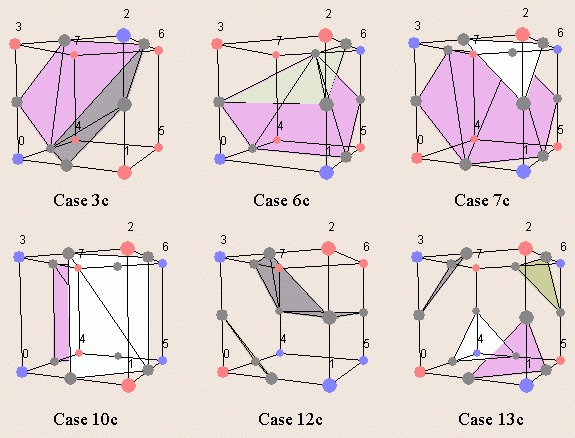
\includegraphics[height=0.65\textwidth,width=0.88\textwidth]{Figures/MC-Ambiguity-solution.jpeg}
\decoRule
\caption{An example of an added complementary cases in Marching Cubes} (\cite{Lingrand_2003})
\label{fig:MC-ambiguity-solution}
\end{figure}

This ambiguity can lead to crashes or holes in the generated surface, especially when neighboring cubes choose different triangulations. Solutions like the Asymptotic Decider (\cite{Nielson_1991}) and Extended Marching Cubes (\cite{Raman_2008}) have been proposed to address these ambiguities (Wang et al., 2020).

\item \textbf{Resolution Dependency:} The resolution of the input scalar field directly affects the quality of the extracted shallow. As displayed in Fig. \ref{fig:MC-sphere-ex} and Fig. \ref{fig:MC-diffrent-resolution}, it is important to note that finer details may be missed at lower resolutions, or the shallow may be excessively smoothed.

\begin{figure}
\centering
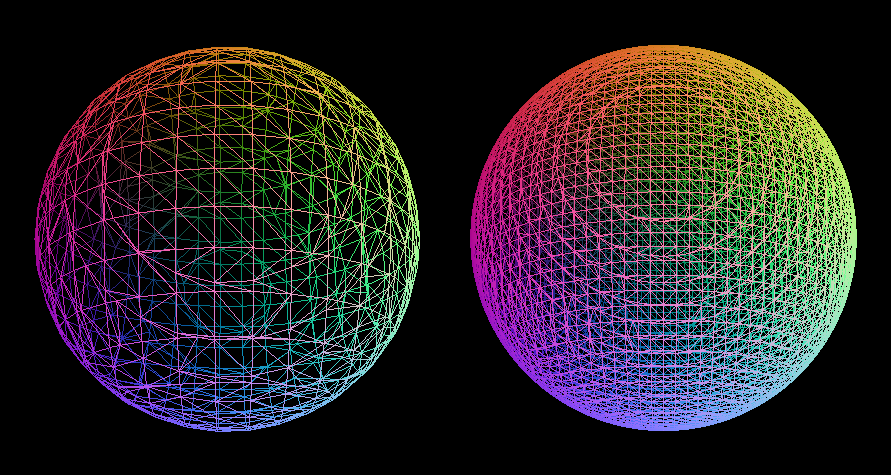
\includegraphics[height=0.5\textwidth,width=0.88\textwidth]{Figures/MarchingCubesSphere.png}
\decoRule
\caption{The comparison of surfaces extracted from the regular cube at two resolutions.} (\cite{Lingrand_2003})
\label{fig:MC-sphere-ex}
\end{figure}

\begin{figure}
\centering
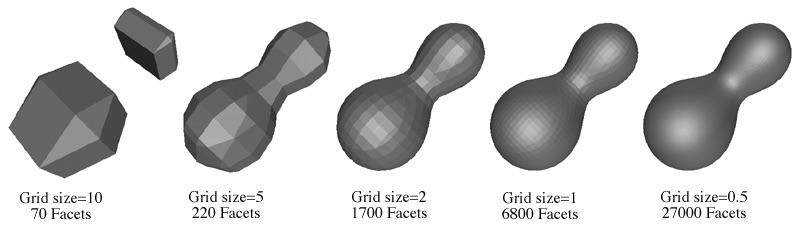
\includegraphics[height=0.3\textwidth,width=\textwidth]{Figures/MC-diffrent-resolution.jpeg}
\decoRule
\caption{The comparison of surfaces extracted at different resolutions. The low-resolution surface misses the finer details present in the high-resolution surface.} (\cite{Bourke_2023})
\label{fig:MC-diffrent-resolution}
\end{figure}

\item \textbf{Lack of Sharp Feature Preservation:} Marching Cubes tend to harvest rounded or smoothed surfaces, even if the original data has sharp features (Fig. \ref{fig:MC-loss-of-sharp-feature}). Methods like Feature-Preserving Marching Cubes have been proposed to address this issue (\cite{Chien-Chang_2005}).

\begin{figure}
\centering
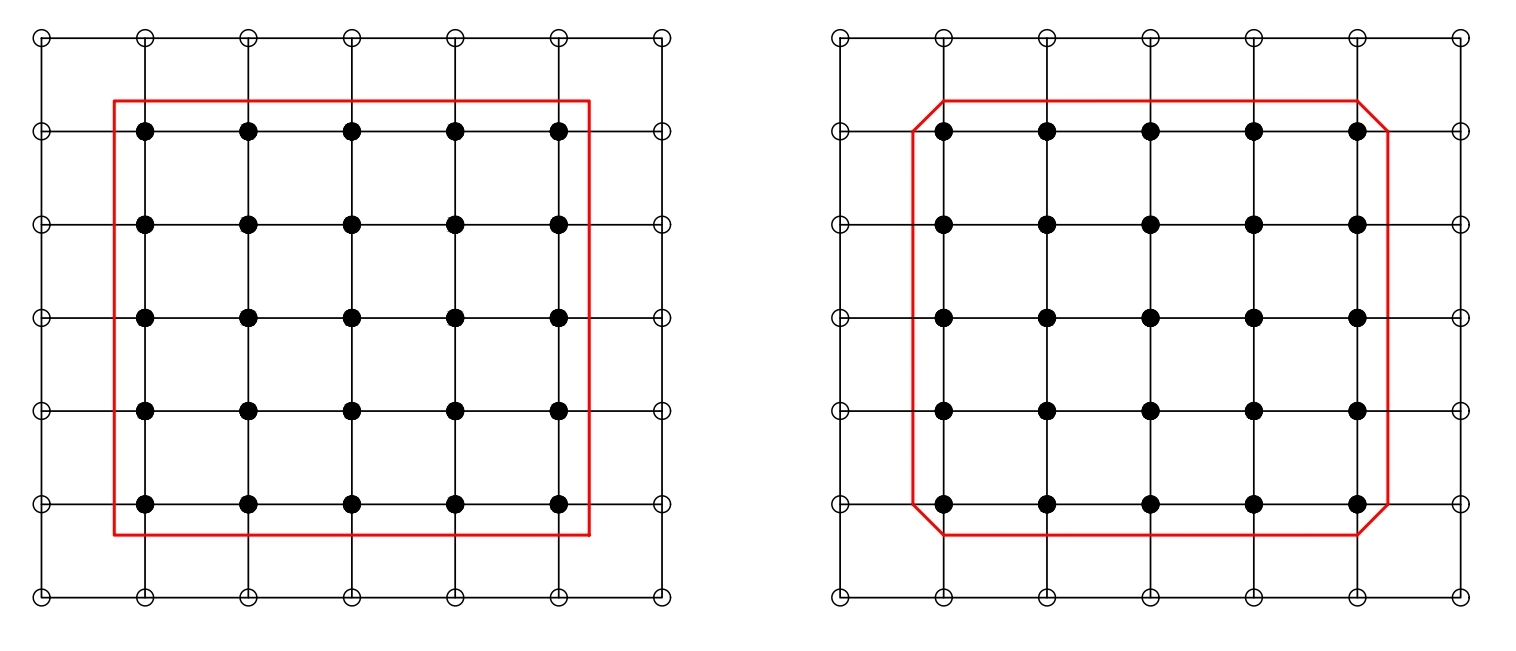
\includegraphics[height=0.45\textwidth,width=\textwidth]{Figures/MC-loss-of-sharp-feature.jpg}
\decoRule
\caption{A sharp feature in the data (left) gets smoothed out in the surface extracted by Marching Cubes (right).} 
\label{fig:MC-loss-of-sharp-feature}
\end{figure}

\end{itemize}

\subsection{Extensions and Variants} 

Over the years, several delays and variants of the MC algorithm have been planned to address its limitations. Some notable ones include Extended Marching Cubes (\cite{Raman_2008}), Asymptotic Decider (\cite{Nielson_1991}), and Dual Marching Cubes (\cite{Nielson_2004}).

\section{Dual Contouring} \label{Dual-Contouring}

Dual Contouring (DC) is an advanced isosurface extraction technique introduced by \cite{Ju_2002}. It was developed as an alternative to the MC algorithm to address some limitations, particularly in preserving sharp features and handling complex topologies. DC has found applications in various fields, including computer graphics, terrain modeling, and scientific visualization, where high-quality surface representations are essential.

\vspace{2mm}
\subsection{Basic Principle}

Unlike MC, which operates on the edges of the grid cells, DC focuses on the grid vertices. The algorithm generates a dual grid, where each cell contains a single vertex, representing the intersection of the isosurface with the cell. This approach allows for better representation of sharp features and complex topologies.

\vspace{2mm}
\subsection{Algorithm Overview}

\begin{itemize}
\item \textbf{Vertex Generation:} 
For each cell in the grid, if the cell intersects the isosurface, a vertex is generated. The optimal position of this vertex is determined by minimizing the Quadratic Error Function (QEF), which measures the error between the vertex position and the isosurface. The QEF is formulated as:
\begin{equation}
QEF(v) = \sum_{i} (n_i \cdot v - d_i)^2
\label{eq:qef}
\end{equation}
Where \( n_i \) is the normal to the isosurface at the \(i^{th}\) intersection point, \( v \) is the vertex position, and \( d_i \) is the signed distance from the origin to the isosurface along the normal \( n_i \) (\cite{Ju_2002}).

\item \textbf{Edge Construction:} Edges are constructed by connecting vertices in adjacent cells. This step ensures that the generated surface is manifold and has no gaps or holes.

\item \textbf{Polygon Construction:} After determining the optimal vertex positions within each cell using the QEF, the next step is connecting these vertices to form polygons representing the isosurface. In Dual Contouring, the polygons are typically quads (Fig. \ref{fig:DC-quad}), but they can be decomposed into triangles for compatibility with most graphics hardware. The connectivity is determined based on the topology of the isosurface intersections within each cell.

\begin{figure}[H]
\centering
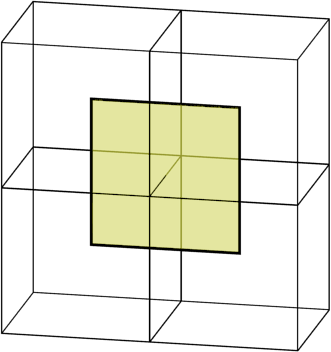
\includegraphics[height=0.5\textwidth,width=0.5\textwidth]{Figures/dc_single_face.png}
\decoRule
\caption{The face is associated with a single edge. It has a point in every adjacent cell.} (\cite{Boristhebrave_2018})
\label{fig:DC-quad}
\end{figure}

\item \textbf{Mesh Refinement:} The initial mesh generated by Dual Contouring might not always be of the desired quality, especially in regions with intricate features or noisy input data. Mesh refinement involves subdividing larger polygons, smoothing vertex positions (while still adhering to the isosurface), and removing artifacts. This step ensures the final mesh is visually appealing and topologically accurate (\cite{Schaefer_2007}).
\end{itemize}

\subsection{Advantages}
\begin{itemize}
\item \textbf{Sharp Feature Preservation:} DC excels in preserving sharp features in the data, which can be smoothed out by algorithms like MC. Figure \ref{fig:DC-MC-compare} shows sharp feature preservation compared to the MC algorithm.

\begin{figure}
\centering
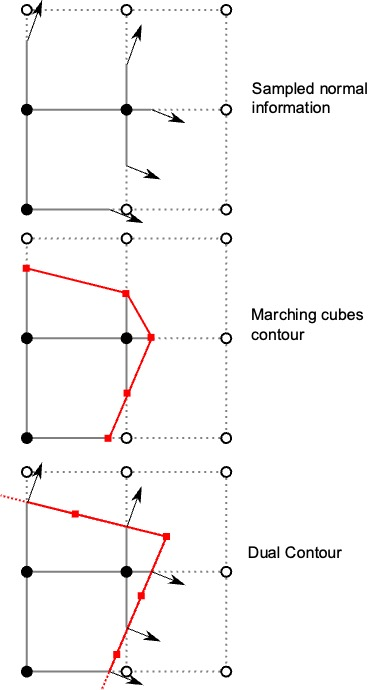
\includegraphics[height=0.95\textwidth, width=0.55\textwidth]{Figures/DC-MC-compare.jpg}
\decoRule
\caption{A signed grid with edge tagged by Hermite data (top), its MC contour (Middle), and its DC contour (bottom)}(\cite{Ju_2002})
\label{fig:DC-MC-compare}
\end{figure}

\item \textbf{Topological Flexibility:} DC can handle complex topologies, ensuring that the generated surface is manifold and does not have gaps or holes.
\end{itemize}

\subsection{Limitations}
\begin{itemize}
\item \textbf{Computational Complexity:} DC can be more computationally intensive than MC, especially for large datasets.

\item \textbf{Memory Consumption:} Due to the dual grid and additional data structures, DC can consume more memory than MC.

\item \textbf{Colinear normals:} 
As described in the original paper (\cite{Ju_2002}), the handling of the QEF is a significant limitation of the Dual Contouring algorithm. When solving the QEF, the aim is to find the point most consistent with the normals of the function. However, there's no guarantee that the resulting point will be inside the cell. As illustrated in Fig. \ref{fig:DC-colinear-ch3}, this issue becomes particularly pronounced in scenarios with large flat surfaces where all the sampled normals are identical or very similar. This issue is discussed extensively in Section \ref{challanges-QEF-minimization} of Chapter \ref{Chapter5}.

\begin{figure}
    \centering
    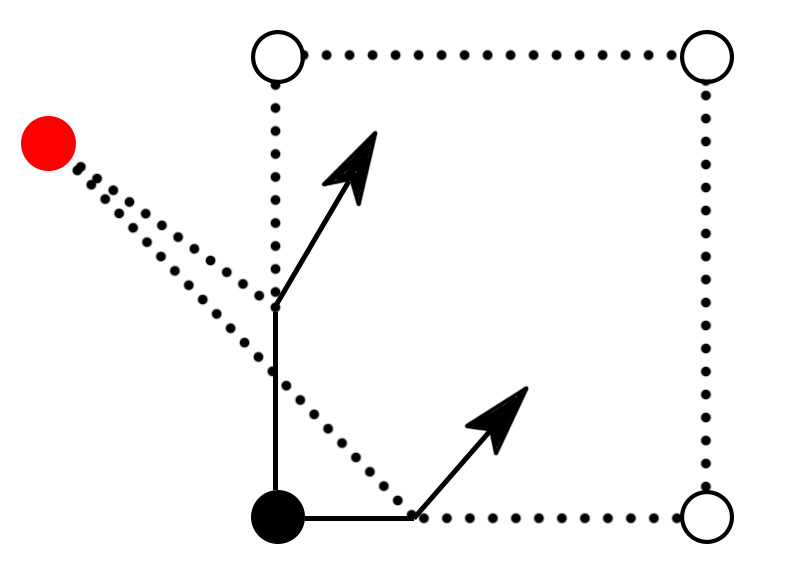
\includegraphics[width=0.4\textwidth]{Figures/DC-colinear.jpg}
    \decoRule
    \caption{Illustration of parallel normals due to a large flat surface.}(\cite{Boristhebrave_2018})
    \label{fig:DC-colinear-ch3}
\end{figure}

\item \textbf{Manifold:} 
While a mesh generated by dual contouring is always watertight, it doesn't always result in a well-defined surface. Given that, there's only one point per cell, situations where two surfaces pass through a single cell will result in them sharing that cell. This phenomenon leads to what's known as a "non-manifold" mesh (Fig. \ref{fig:DC-manifold}). 

\begin{figure}
\centering
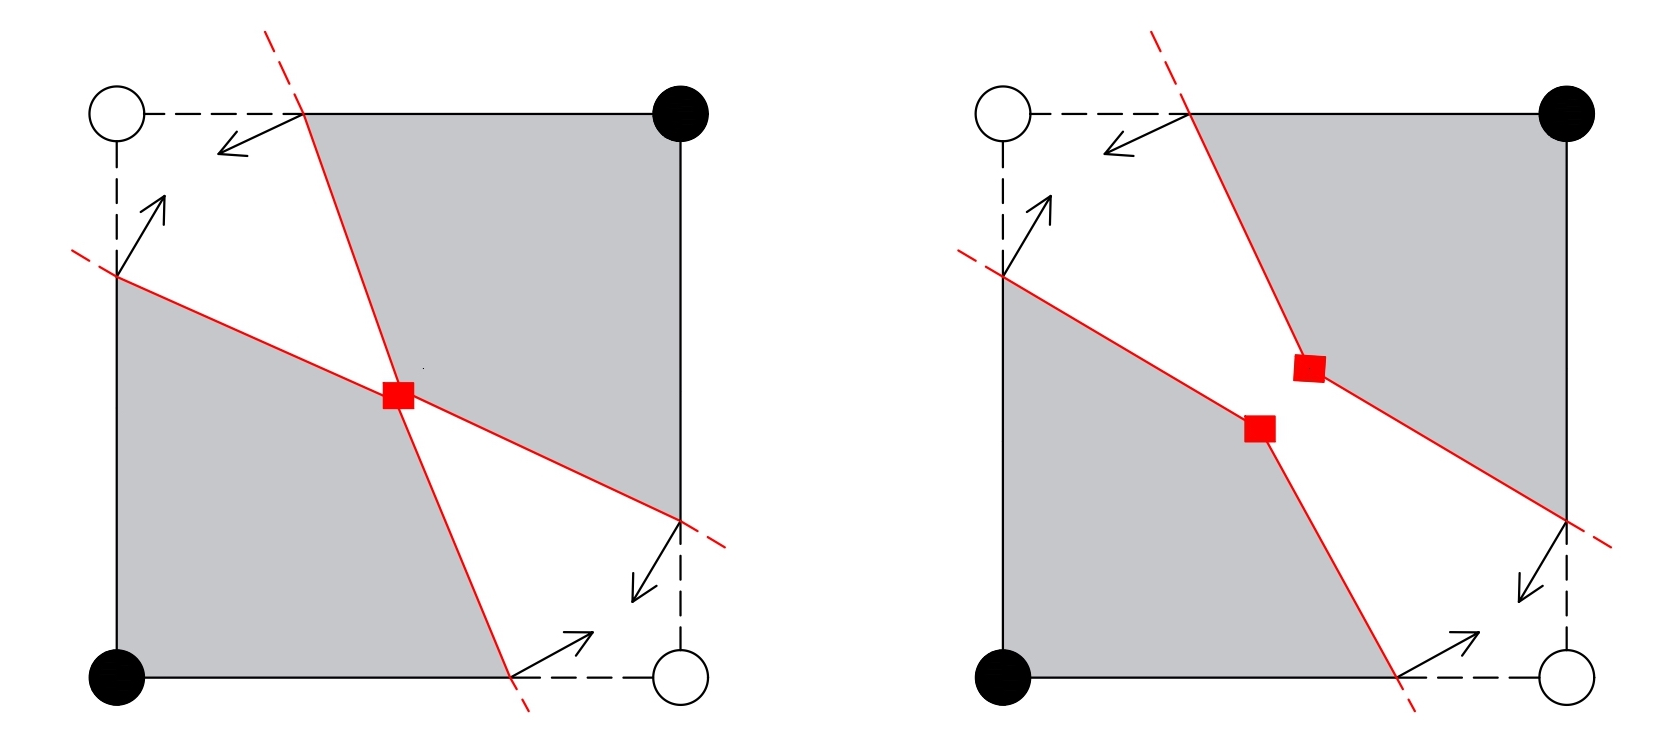
\includegraphics[width=0.7\textwidth]{Figures/DC-manifold.jpg}
\decoRule
\caption{A limitation of the DC algorithm is that it permits only one point per cell (left). An optimal solution for a given scenario would require two vertexes (right).}(\cite{Boristhebrave_2018})
\label{fig:DC-manifold}
\end{figure}

Non-manifold meshes can interfere with certain texturing algorithms and are particularly prevalent in scenarios where solids are thinner than the cell size or when multiple objects are in close proximity to each other (\cite{Schaefer_2007}).

\item \textbf{Mesh Quality:} While DC preserves sharp features, it can sometimes produce jagged or noisy surfaces, especially if the input data is not clean or well-sampled (\cite{Zhang_2004}).

\item \textbf{Inability to Generate Thin Features:} As illustrated in Fig. \ref{fig:DC-thin-brick} and Fig. \ref{fig:DC-think-brick-mesh}, one of the main limitations of DC is its difficulty in generating thin features in the mesh. This limitation arises because the dual contouring algorithm only allows one vertex per cell, which inherently restricts the representation of thin structures. This can lead to a loss of detail in specific datasets where thin structures are crucial (\cite{Zhang_2004}).

\begin{figure}
\centering
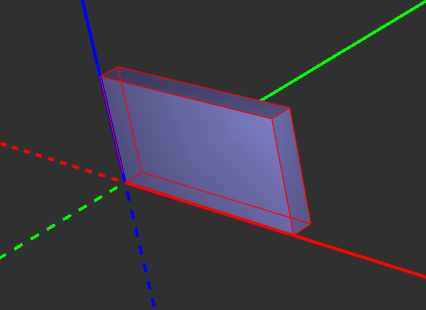
\includegraphics[height=0.7\textwidth, width=0.8\textwidth]{Figures/Thin-brick.png}
\decoRule
\caption{Analyzing the DC algorithm when the object's width is smaller than the width of the cell.}
\label{fig:DC-thin-brick}
\end{figure}

\begin{figure}
\centering
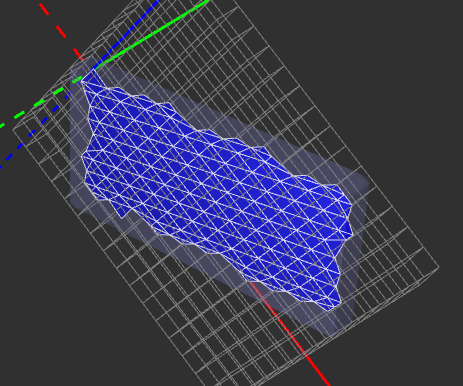
\includegraphics[height=0.7\textwidth, width=0.8\textwidth]{Figures/DC-thin-brick-mesh.png}
\decoRule
\caption{As a consequence, the DC algorithm fails to produce thin features, leading to the generation of infinitely thin sheet.}
\label{fig:DC-think-brick-mesh}
\end{figure}
\end{itemize}

\subsection{Extensions and Variants}

Several extensions and variants of the DC algorithm have been proposed to address its limitations and improve its performance. Notable ones include Adaptive Dual Contouring, Simplified Dual Contouring, and Feature-Preserving Dual Contouring (\cite{Zhang_2004}).

\section{Cubical Marching Squares} \label{Cubical-Marching-Squares}

The Cubical Marching Squares (CMS) algorithm, as introduced by \cite{Chien-Chang_2005}, represents an evolution of the Marching Squares and Marching Cubes algorithms. Designed to extract isosurfaces from 3D scalar fields, CMS emphasizes adaptability and feature preservation, making it a significant advancement in the field of isosurface extraction.

\vspace{2mm}
\subsection{Basic Principle}

The Cubical Marching Squares (CMS) algorithm enhances traditional isosurface extraction techniques, aiming to represent a three-dimensional scalar field as a two-dimensional isosurface. Building on the principles of Marching Cubes, CMS introduces adaptability. Rather than uniformly processing the scalar field, it adjusts its resolution based on data complexity. This ensures that intricate features are captured in detail while simpler areas are efficiently processed, making CMS adept at producing detailed and accurate representations of 3D scalar fields (\cite{Chien-Chang_2005}).

\vspace{2mm}
\subsection{Algorithm Overview}

The Cubical Marching Squares (CMS) algorithm is a methodical process that combines the principles of Marching Squares and Marching Cubes (\cite{Lorensen_1987}), refining them with an adaptive approach to better capture the intricacies of 3D scalar fields. Here's a more detailed breakdown:

\begin{itemize}
\item \textbf{Initialization:}
The CMS algorithm initiates by segmenting the 3D scalar field into a grid of cubes reminiscent of the Marching Cubes approach. Each corner of these cubes undergoes sampling to ascertain their scalar values.

\item \textbf{Adaptive Subdivision:}
Diverging from the uniform operation of traditional Marching Cubes, CMS evaluates the variance of scalar values within each cube. When this variance exceeds a predefined threshold, signaling the presence of a potential feature or sharp transition, the cube is subjected to subdivision. This recursive adaptive process continues until the variance within each subdivided cube either falls below the threshold or reaches a predetermined maximum subdivision level (\cite{Chien-Chang_2005}).

\item \textbf{Feature Preservation:}
The algorithm calculates the gradient at each corner for each cube (or subdivided cube), approximating the surface normal. These normals are crucial in determining the optimal position of the vertex within the cube, ensuring that sharp features are well-represented.

\item \textbf{Lookup Tables and Vertex Positioning:}
A specific configuration is identified based on the scalar values at the corners of each cube. Using this configuration, the algorithm employs a lookup table to determine how the cube should be triangulated.

\item \textbf{Edge Construction and Isosurface Generation:}
As illustrated in Fig. \ref{fig:CMS}, a cube possesses six faces. The isocurve or the isosurface is generated using the Marching Cubes algorithm for each face. The isocurve produced consists of multiple segments for each face. Components akin to the MC are obtained when these segments are properly connected and reverted to the original cube. Edges are formed by linking vertices in adjacent cubes, serving as the foundation for the isosurface construction.

\begin{figure}
\centering
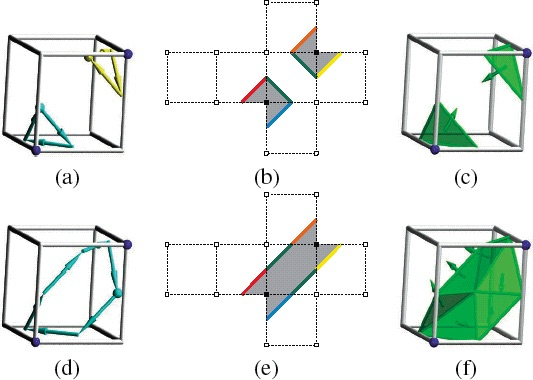
\includegraphics[width=0.85\textwidth]{Figures/CMS.jpeg}
\decoRule
\caption{Cubical Marching Squares illustration. A cube (a, d) unfolds into six squares (b, e). Each square is processed, and segments are returned to 3D to form components (a, d). Ambiguities are resolved in 2D, and the components are triangulated to form the isosurface (c, f).}(\cite{Chien-Chang_2005})
\label{fig:CMS}
\end{figure}

\item \textbf{Polygon Construction and Triangulation:}
The process of refining the isosurface involves triangulation. While the method chosen for triangulation can vary, it must remain consistent throughout the process. The term "cubical marching squares" arises from the ability to convert a single lookup table used in the Marching Cubes algorithm into six separate lookup tables used in the Marching Squares algorithm. While Marching Squares may be slower than Marching Cubes, it eliminates dependencies between cells by focusing on sharp features on the faces of cubes (\cite{Sreeparna_2017}).

\begin{figure}
\centering
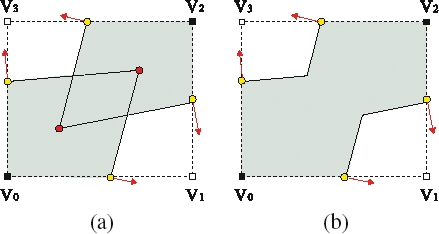
\includegraphics[width=0.75\textwidth]{Figures/CMS-Ambiguty.jpg}
\decoRule
\caption{A cell face that has intersecting sharp features. Self-intersection (a) should not happen in a volume; therefore, the algorithm chooses the correct disambiguated configuration (b) with preserved sharp features.}(\cite{Chien-Chang_2005})
\label{fig:CMS-Ambiguity}
\end{figure}

Challenges arise when determining the relationship between two components based solely on the signs of their vertices, leading to internal ambiguities. These ambiguities, which resemble face ambiguities, can be addressed using 3D sharp features. If two components have overlapping volumes, they are deemed connected; if not, they are treated as separate entities (Fig. \ref{fig:CMS-Ambiguity}). For each separate component, a triangle fan is constructed. In cases where two components are interconnected, the resulting surface takes on a cylindrical shape. For these scenarios, employing a dynamic programming approach is effective for triangulation and connecting components to create the final surface (\cite{Sreeparna_2017}).
\end{itemize}

\subsection{Advantages}
\begin{itemize}
\item \textbf{Higher Quality Meshes:} The adaptive nature of CMS allows for the production of meshes that more accurately represent the underlying scalar field, especially in regions with sharp features. Its flexibility ensures superior quality representations, giving it a distinct advantage over traditional methods.
\item \textbf{Efficiency:} As noted by \cite{Chien-Chang_2005}, CMS often generates fewer triangles than conventional Marching Cubes while achieving a similar or even superior level of detail, thanks to its adaptive subdivision of the scalar field.
\end{itemize}

\subsection{Limitations}
\begin{itemize}
\item \textbf{Complexity:} The algorithm's adaptive nature and the enhanced lookup tables introduce a higher complexity level than the traditional Marching Cubes.
\item \textbf{Ambiguities:} While CMS addresses many of the topological ambiguities inherent in Marching Cubes, certain configurations can still pose challenges. These ambiguities, discussed in the context of Marching Cubes by \cite{Nielson_1991}, continue to concern advanced algorithms like CMS.
\end{itemize}

\subsection{Applications}

Owing to its capability to capture sharp features and adapt to the underlying data, CMS has been employed in areas demanding high-quality surface representations. These include medical imaging, geophysics, and scientific visualization.


\section{Dual Marching Cubes} \label{Dual-Marching-Cubes}

The Dual Marching Cubes (DMC) algorithm, introduced by \cite{Nielson_2004}, is an evolution of the Marching Cubes and Dual Contouring algorithms. It aims to combine the strengths of both methods to produce high-quality isosurfaces from 3D scalar fields. The DMC algorithm is mainly known for its ability to generate adaptive and topologically accurate meshes, making it a significant advancement in the realm of isosurface extraction.

\vspace{2mm}
\subsection{Basic Principle}

DMC operates by constructing a dual grid from the original scalar field grid. Each cell corresponds to a vertex in the original grid in this dual grid. The algorithm generates vertices at optimal positions within each voxel of the dual grid, ensuring that the resulting mesh closely adheres to the underlying scalar field. By combining the adaptability of Dual Contouring with the robustness of Marching Cubes, DMC aims to produce isosurfaces that are detailed and topologically accurate (\cite{Schaefer_2004}).

\vspace{2mm}
\subsection{Algorithm Overview}

The Dual Marching Cubes algorithm is an advanced method that builds upon the principles of Marching Cubes but operates on a topologically dual grid to the structured grids used by other techniques. It aims to generate a mesh that closely represents the underlying scalar field while ensuring topological accuracy and adaptability. Here is a more detailed breakdown:

\begin{itemize}
\item \textbf{Initialization and Dual Grid Construction:}
The algorithm begins with a structured grid, often referred to as the Primal grid, that adaptively samples the function. From this primal grid, a dual grid is derived. The vertices of the dual grid are determined by the Quadratic Error Function calculations, pinpointing the features within each grid cell. This dual grid aligns with the function's features, and the surface is subsequently generated using a generalized version of Marching Cubes (\cite{Schaefer_2004}).

\begin{figure}[H]
\centering
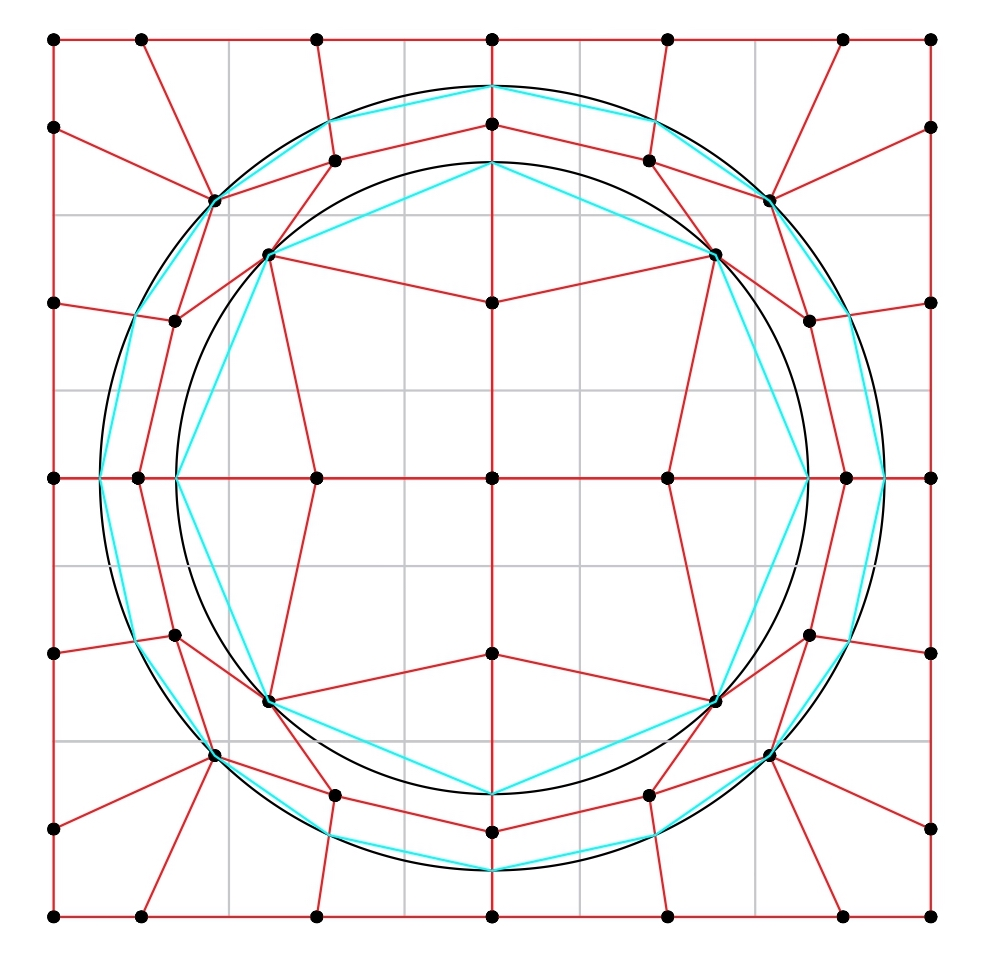
\includegraphics[height=0.75\textwidth,width=0.8\textwidth]{Figures/DMC-dual-grid.jpg}
\decoRule
\caption{2D visualization of the Dual Marching Cubes Algorithm on a thin torus}
\label{fig:DMC-dual-grid-ex}
\end{figure}

In the illustrated Fig. \ref{fig:DMC-dual-grid-ex}, the dual grid's formation in the Dual Marching Cubes algorithm is highlighted. The primal grid is shown in light grey, and the dual grid, constructed by connecting the QEF points, is emphasized in contrasting red. These QEF points are marked as black vertices. A comprehensive understanding of the dual grid's role and importance in the DMC algorithm can be found in Chapter \ref{Chapter6}.

\item \textbf{Scalar Field Analysis:}
Before diving into vertex generation, the algorithm analyzes the scalar field within each voxel. This involves determining if the voxel intersects the isosurface by checking if the scalar values at its corners span the desired isovalue. If an intersection is detected, the voxel is flagged for further processing.

\item \textbf{Feature Isolation and Vertex Generation:}
The Quadratic Error Function is used to determine the vertex that approximates the feature of the function inside a cell. This QEF is generated by computing tangent planes to the graph of the function on a grid of points sampled over the cell. The QEF is then minimized over the cell to find the vertex of the dual grid.

\item \textbf{Topology Creation:}
Once a grid is established and feature isolation generates the vertices of the dual grid, the next step is to generate the topology of the dual grid. This dual grid is topologically dual to the primal grid. A cell in the dual grid is created for every vertex in the grid. The vertices of this cell are the feature vertices inside each cube in the grid containing that vertex (\cite{Schaefer_2004}).

\item \textbf{Polygon Construction and Triangulation:}
After the topology creation, the algorithm forms polygons representing the isosurface. In DMC, these polygons are typically quads. However, these quads can be further divided into triangles for compatibility with most graphics hardware. The triangulation is guided by the scalar values at the voxel corners and the topology of the isosurface intersections within each voxel.

\item \textbf{Mesh Refinement and Post-processing:}
While topologically accurate, the initial mesh generated by DMC might require further refinement to enhance its visual quality. This involves subdividing larger polygons, smoothing vertex positions, and removing artifacts. The refinement ensures the final mesh is topologically accurate and visually appealing, making it suitable for various applications.
\end{itemize}

\vspace{2mm}
\subsection{Advantages}
\begin{itemize}
\item \textbf{Sharp Feature Preservation:} One of the standout features of DMC is its ability to reproduce sharp features such as edges and corners. Traditional methods might smooth out or miss these features, but DMC, by aligning vertices with the features of the implicit function, ensures that these sharp features are accurately represented in the generated mesh (Fig. \ref{fig:DMC}).

\item \textbf{Efficient Representation of Thin Structures:} DMC excels in representing both thin-walled structures and intricate thin features, as evident in Fig. \ref{fig:DMC}. Compared to other methods, DMC can generate a polygonal approximation with significantly fewer polygons, making it particularly advantageous for scenarios where the thickness or fineness of structures is a critical factor (Fig. \ref{fig:DMC-compare}). This capability ensures that both large-scale thin walls and minute details are captured without the need for excessive grid subdivision, a challenge that other algorithms might struggle with or require a much finer grid to address (\cite{Schaefer_2004}).

\begin{figure}
\centering
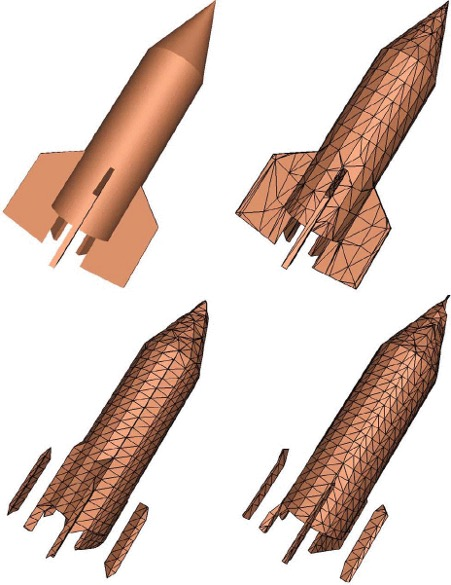
\includegraphics[height=0.6\textwidth, width=0.6\textwidth]{Figures/DMC.jpg}
\decoRule
\caption{CSG model of a rocket (upper left) and models approximating the shape using the same number of polygons. Dual Marching Cubes (upper right), Marching Cubes (lower left), and Dual Contouring (lower right).}(\cite{Schaefer_2004})
\label{fig:DMC}
\end{figure}

\begin{figure}[t]
\centering
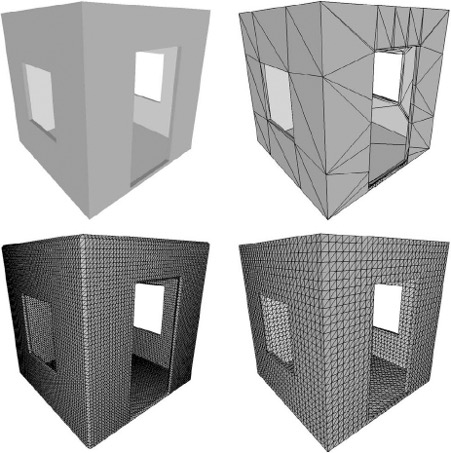
\includegraphics[height=0.6\textwidth, width=0.6\textwidth]{Figures/DMC-compare.jpg}
\decoRule
\caption{A thin-walled room defined via CSG (upper left). Polygonal approximations were generated by Marching Cubes (lower left, 67K polys), Dual Contouring (lower right, 17K polys), and Dual Marching Cubes (upper right, 440 polys). Using Dual Marching Cubes, the size of the contour mesh is insensitive to the thickness of the walls}(\cite{Schaefer_2004})
\label{fig:DMC-compare}
\end{figure}

\item \textbf{Topological Accuracy:} DMC ensures the generated mesh is topologically manifold, free from gaps, holes, or inconsistencies. This is crucial for many applications, especially in scientific visualization and computer graphics.

\item \textbf{Crack-free Mesh:} The algorithm ensures that the generated mesh is crack-free, eliminating the common problem of small gaps or inconsistencies that can arise in mesh generation.

\item \textbf{Scalability:} DMC is designed to handle large datasets efficiently, making it suitable for applications that deal with extensive volumetric data, such as medical imaging or geological studies.
\end{itemize}

\subsection{Limitations}

\begin{itemize}
\item \textbf{Computational Intensity:} One of the primary limitations of DMC is its computational demand. The algorithm can be computationally heavy, especially when aiming to capture intricate details and sharp features. This might lead to longer processing times, especially for large datasets.

\item \textbf{Complex Implementation:} The DMC algorithm, focusing on capturing sharp and thin features, can be more complex than traditional Marching Cubes. This complexity can pose developers challenges and lead to potential bugs if not implemented carefully.

\item \textbf{Dependency on Quality of Input Data:} The accuracy and quality of the generated mesh heavily depend on the quality of the input scalar field. Noisy or imprecise data can lead to sub-optimal results.

\item \textbf{Difficulty in Real-time Applications:} Due to its computational demands, using DMC in real-time applications, such as games or interactive simulations, can be challenging.

\item \textbf{Optimization Challenges:} While DMC aims to minimize errors using Quadratic Error Functions, finding the global minimum can be challenging, and the algorithm might sometimes settle for local minima, leading to sub-optimal vertex placements.
\end{itemize}

\subsection{Applications}

DMC's ability to produce detailed and topologically accurate isosurfaces has led to its adoption in various fields requiring high-quality surface representations. These include medical imaging, geophysics, and scientific visualization.

\section{Comparative Analysis of Methods}

This section will compare the discussed isosurface extraction methods, namely Marching Squares (MS), Marching Cubes (MC), Dual Contouring (DC), Cubical Marching Squares (CMS), and Dual Marching Cubes (DMC), based on various criteria.

\noindent \textbf{Mesh Quality:}
\begin{itemize}
\item \textbf{MS:} Provides a straightforward representation exclusively for 2D scalar fields. With the integration of a quadtree structure, it can adeptly capture intricate details.
\item \textbf{MC:} Produces a consistent mesh but often lacks in preserving sharp features. The mesh quality directly depends on the resolution of the input scalar field.
\item \textbf{DC:} Known for preserving sharp features, but the calculation for QEF can be tricky and cannot reproduce the thin features.
\item \textbf{CMS:} Produces high-quality meshes, especially in regions with sharp features, due to its adaptive nature.
\item \textbf{DMC:} Generates meshes closely representing the underlying scalar field, ensuring detail, topological accuracy, and the ability to represent thin surfaces or features that other methods might miss.
\end{itemize}

\noindent \textbf{Computational Efficiency:}
\begin{itemize}
\item \textbf{MS:} Efficient for 2D datasets with regular grid, but might require more computational resources when adapted for quadtree implementation.
\item \textbf{MC:} Relatively fast and can be applied in real-time for specific applications.
\item \textbf{DC:} More computationally intensive than MC due to QEF calculations, especially for large datasets.
\item \textbf{CMS:} Efficient in producing fewer triangles than MC for a similar level of detail.
\item \textbf{DMC:} While efficiently capturing details, it can be computationally demanding due to the dual grid construction and QEF minimization.
\end{itemize}

\noindent \textbf{Topological Accuracy:}
\begin{itemize}
\item \textbf{MS:} It ensures topological accuracy within 2D domains, faithfully representing the contours of scalar fields.
\item \textbf{MC:} Recognized for its inherent ambiguities, the method often encounters challenges in accurately representing complex topologies. These ambiguities can manifest as inconsistencies in the mesh. 
\item \textbf{DC:} Handles complex topologies well, ensuring the generated surface is manifold.
\item \textbf{CMS:} Addresses many topological ambiguities inherent in MC but still has some challenges.
\item \textbf{DMC:} Ensures topological accuracy by focusing on the dual grid, making it robust against topological errors and adept at representing thin features.
\end{itemize}

\noindent \textbf{Adaptability:}
\begin{itemize}
\item \textbf{MS:} It is designed exclusively for 2D fields, so its adaptability is confined to this dimension.
\item \textbf{MC:} Processes the scalar field uniformly, leading to potential loss of detail in complex regions.
\item \textbf{DC:} Focuses on grid vertices, allowing for better representation of sharp features.
\item \textbf{CMS:} Highly adaptive, adjusting its resolution based on data complexity.
\item \textbf{DMC:} Combines the strengths of MC and DC, ensuring adaptability, detail preservation, and the unique capability to represent thin surfaces or features.
\end{itemize}

\section{Summary}
Isosurface extraction is a pivotal technique in computer graphics, medical imaging, geophysics, and scientific visualization. The methods discussed in this chapter, namely Marching Cubes, Dual Contouring, Cubical Marching Squares, and Dual Marching Cubes, offer unique advantages and have specific limitations (Table \ref{table:comparison-of-methods}). 

\renewcommand{\arraystretch}{1.5}
\begin{table}[H]
\centering
\begin{tabular}{l|c|c|c|c|c}
 & MS & MC & DC & CMS & DMC \\
\hline
Easy to Implement & $\checkmark$ $\checkmark$ & - & - & - & - \\
Local Independence & $\checkmark$ & $\checkmark$ & - & $\checkmark$ & - \\
Smooth & - & $\checkmark$ & $\checkmark$ & $\checkmark$ & $\checkmark$ \\
Adaptive & - & - & $\checkmark$ & $\checkmark$ & $\checkmark$ \\
Minimize slivers & $\checkmark$ & - & $\checkmark$ & $\checkmark$ & $\checkmark$ \\
Sharp features & - & - & $\checkmark$ & $\checkmark$ & $\checkmark$ \\
Thin features & - & - & - & $ \sim $ & $\checkmark$ \\
\end{tabular}
\caption{Comparison of methods based on criteria. \\
$ \sim $  CMS is capable of representing thin features when utilized with octree adaptation and a grid of sufficiently fine resolution.
} \label{table:comparison-of-methods}
\end{table}

Marching Cubes, being one of the earliest methods, laid the foundation for isosurface extraction. However, its inability to preserve sharp features and handle complex topologies led to the development of advanced techniques like Dual Contouring and Cubical Marching Squares. Dual Contouring, while excelling at preserving sharp features, struggles with producing thin features and can be computationally intensive. On the other hand, Cubical Marching Squares introduces adaptability, ensuring detailed representation in complex regions while efficient in simpler areas. Dual Marching Cubes combines the strengths of both MC and DC, ensuring detail preservation, topological accuracy, and the capability to represent thin features that Dual Contouring lacks.

Choosing the right method depends on the application's specific requirements, the nature of the data, and the computational resources available. As research progresses in this domain, we can expect further refinements and new techniques that address the existing limitations and offer even more accurate and efficient isosurface extraction methods.
\chapter{Embree API Integration: Ray Tracing and Mesh Data Structures} \label{Chapter4}

\section{Problem Formulation} \label{sec:Problem Formulation}
Isosurface extraction is a fundamental process in computer graphics and scientific visualization. It generates an isosurface representing a particular scalar value within a three-dimensional field. This scalar field can be derived from various sources, such as medical imaging data, geospatial datasets, or computational fluid dynamics simulations.

The primary challenge in isosurface extraction is to generate a mesh that accurately represents the underlying data. This mesh should capture the intricate details of the scalar field and be computationally efficient to render and process.

\subsection{Mesh Generation} The quality of the generated mesh is paramount. An ideal mesh should:

\begin{itemize}
    \item Accurately represent the scalar field's features, both large and small.
    \item Preserve sharp features without introducing artifacts.
    \item Be topologically consistent and watertight, ensuring no gaps or overlaps in the mesh.
    \item Minimize the number of polygons or triangles, ensuring computational efficiency.
\end{itemize}

However, achieving all these objectives simultaneously is challenging. Traditional methods like Marching Cubes can generate consistent meshes but often fail to preserve sharp features, as discussed in Section \ref{Marching-Cubes}. The Dual Contouring algorithm addresses some limitations by preserving sharp features but can struggle with thin features, as explained in Section \ref{Dual-Contouring}.

\subsection{The Dual Marching Cubes Solution} 

Recognizing the strengths and weaknesses of Marching Cubes and Dual Contouring, the Dual Marching Cubes algorithm emerges as a comprehensive solution. By combining the consistent meshing capabilities of Marching Cubes with the sharp feature preservation of Dual Contouring, Dual Marching Cubes aims to generate high-quality meshes that are both accurate and computationally efficient.

\subsection{The Essence of Dual Marching Cubes}

At the heart of the Dual Marching Cubes algorithm lies the dual grid. This grid is constructed by connecting the Quadratic Error Function minimizer points generated during the Dual Contouring process. The dual grid bridges the consistent meshing capabilities of Marching Cubes and the sharp feature preservation of Dual Contouring. By leveraging this dual grid, Dual Marching Cubes can generate meshes that capture the intricate details of the scalar field while ensuring computational efficiency.

\subsection{Implementation of DC and DMC} 

Recognizing the challenges and the potential of Dual Contouring and Dual Marching Cubes, both algorithms were implemented in this work. The implementation aimed to address the known limitations of each algorithm while leveraging their strengths. The subsequent sections delve into the intricacies of this implementation, highlighting the software tools used, the data structures employed, and the validation and testing approach adopted.

\subsection{Summary}

This section laid the groundwork for understanding the complexities involved in isosurface extraction, a critical operation in medical imaging to computational fluid dynamics. The primary challenge lies in generating an accurate and computationally efficient mesh. Traditional methods like Marching Cubes and Dual Contouring offer partial solutions but have limitations.

The Dual Marching Cubes algorithm is introduced as a comprehensive solution that combines the strengths of both Marching Cubes and Dual Contouring. It leverages a dual grid system to balance mesh consistency and feature preservation. Implementing these algorithms, particularly Dual Marching Cubes forms the core of the thesis, which aims to address the challenges outlined here.

The subsequent sections will delve deeper into the implementation details of the Quadratic Error Function, the software tools utilized, and the approaches taken to overcome the challenges in calculating the Quadratic Error Function.

\section{Data Structures} \label{Data-Structures}

Implementing the Dual Marching Cubes algorithm and integrating it with the Intel Embree API necessitated the design of specific data structures to store and process the required data efficiently. This section provides an overview of these structures and their significance in the algorithm. Below, we delve into each of these data structures, elucidating their design and purpose in the context of the algorithm.

\subsection{CartesianMeshIntersectionData}

The structure \ref{lst:CartesianMeshIntersectionData} is pivotal for the ray tracing process. Whenever a ray intersects with a geometry, the \texttt{embreeHitFilter} function is invoked, populating the CartesianMeshIntersectionData structure with intersection details.

\vspace{2mm}
\begin{lstlisting}[language=C++, caption=CartesianMeshIntersectionData structure, label=lst:CartesianMeshIntersectionData]
struct CartesianMeshIntersectionData
{
    unsigned int hitCount;  // Count of intersections
    float lastDistance;  // Distance to the last intersection
    unsigned int lastPrimID;  // Primitive ID of the last intersection
    std::vector<vector3> hitPoints;  // Vector storing the intersection points
    std::vector<vector3> hitNormals;  // Vector storing the normals at the intersection points
};
\end{lstlisting}


\subsection{PrimalGridCell} \label{PrimalGridCell}

The \texttt{PrimalGridCell} structure (Listing \ref{lst:PrimalGridCell}) represents each cell of the primal grid used in the Dual Contouring process. It stores intersection points, normals, and other essential data for each cell.

\vspace{2mm}
\begin{lstlisting}[language=C++, caption=PrimalGridCell structure, label=lst:PrimalGridCell]
struct PrimalGridCell 
{
    std::vector<vector3> hitPoints;  // Vector storing the intersection points within the cell
    std::vector<vector3> hitNormals; // Vector storing the normals at the intersection points within the cell
    vector3 cellMinPoint; // Minimum point (corner) of the cell
    vector3 cellMaxPoint; // Maximum point (corner) of the cell
    vector3 averagePoint; // Average point of the cell
    vector3 QEFPoint;  // Point that minimizes the QEF within the cell
};
\end{lstlisting}


This structure is utilized as a 3D mesh, with each cell storing the intersection details pertinent to its region.

\subsection{DualGridCell} \label{DualGridCell}

The \texttt{DualGridCell} structure (Listing \ref{lst:DualGridCell}) represents each cell of the dual grid. The vertices of the dual grid are the QEF points, which are crucial for the Dual Marching Cubes algorithm.

\vspace{2mm}
\begin{lstlisting}[language=C++, caption=DualGridCell structure, label=lst:DualGridCell]
struct DualGridCell
{
    std::vector<vector3> vertices;  // Vector storing the eight vertices of the dual grid cell
    std::vector<double> scalarFieldValues;  // Vector storing the scalar field values at each vertex
    unsigned int cubeIndex;  // Index representing the cube configuration based on the scalar field

    DualGridCell() : vertices(8, vector3::Empty()), scalarFieldValues(8, 0.0), cubeIndex(0) {}  // Constructor initializing the vectors and cube index
};
\end{lstlisting}

This structure is also used as a 3D mesh, with each cell storing the vertices and scalar field values pertinent to its region. The scalar field value at a given vertex indicates whether that vertex is inside (represented by a value of 1.0) or outside (represented by a value of 0.0) a particular shape or boundary. This distinction is essential for the algorithm, as it determines how the mesh contours around the shape. The cubeIndex is an integral representation of the cell's configuration based on these scalar field values. It plays a crucial role in determining the triangulation pattern for the cell. A more detailed explanation of how these values are populated and their significance can be found in Section \ref{populating-dual-grid}.


\subsection{MeshLines and PaddedMeshLines} \label{meshLines}

The \texttt{meshLines} represent the discrete lines or divisions within the grid, forming the skeleton of the 3D mesh. These lines are crucial for determining the boundaries of each cell in the grid and for facilitating the traversal and processing of the grid's data.

\noindent \begin{itemize}
\item \textbf{meshLinesX, meshLinesY, and meshLinesZ} 
    
These represent the divisions in the X, Y, and Z directions, respectively. They define the structure of the primal grid and dictate how the data is segmented within the 3D space.

\end{itemize}

\noindent However, when working with 3D grids, boundary cases can pose challenges. These are scenarios where a computation or operation is at the edge or limit of the grid. Handling boundary cases often requires additional logic or conditions, which can complicate the algorithm and potentially slow its execution.

\noindent \begin{itemize}
\item \textbf{paddedMeshLinesX, paddedMeshLinesY, and paddedMeshLinesZ} 

To address the issue with boundaries, \texttt{paddedMeshLines} are introduced. The \texttt{paddedMeshLines} are essentially the \texttt{meshLines} but with an added layer or "padding" in each direction. This padding helps avoid boundary cases by ensuring that all operations are safely within the bounds of the grid.

These represent the padded divisions in the X, Y, and Z directions. The padding is achieved by adding one step in each direction to the original \texttt{meshLines}.

\end{itemize}

\subsubsection{Advantages of Using PaddedMeshLines}

\begin{itemize}
    \item \textbf{Simplified Logic:} By avoiding boundary cases, the logic is more straightforward, reducing the chances of errors.
    \item \textbf{Performance:} Without constantly checking for boundary conditions, the algorithm can run more efficiently.
    \item \textbf{Flexibility:} The padding provides a buffer, ensuring that even if data points are close to the edge, they can be processed without special conditions.
    \item \textbf{Consistency:} All cells, including those at the boundaries, are treated uniformly, ensuring consistent results across the grid.
\end{itemize}

In essence, while \texttt{meshLines} provide the fundamental structure of the 3D grid, the \texttt{paddedMeshLines} offer an enhanced framework that simplifies the processing and ensures consistent and efficient operations throughout the grid.

\subsection{Nested Vector Mesh Representation}

For both the primal and dual grids, a 3D mesh representation is essential to store and process the data efficiently. This 3D mesh is realized using a nested vector list, essentially a 2D vector list extended to represent three dimensions.

\subsubsection{Primal Grid Mesh} \label{Primal-Grid-Mesh}

The primal grid's 3D mesh is constructed using a nested vector list (Listing \ref{lst:primalGrid}), where each cell of the mesh is an instance of the \texttt{PrimalGridCell} structure. This nested structure allows for efficient traversal and data access, ensuring that the algorithm can quickly retrieve and process the intersection details for each cell.

\vspace{1mm}
\begin{lstlisting}[language=C++, caption=3D Mesh Representation Using Primal Grid Cells, label=lst:primalGrid]
std::vector<std::vector<std::vector<PrimalGridCell>>> primalGrid(
    meshLinesX.size() - 1,
    std::vector<std::vector<PrimalGridCell>>(
        meshLinesY.size() - 1, 
        std::vector<PrimalGridCell>(meshLinesZ.size() - 1)
    )
);
\end{lstlisting}

\subsubsection{Dual Grid Mesh} \label{Dual-Grid-Mesh}

Similarly, the dual grid's 3D mesh is also constructed using a nested vector list (Listing \ref{lst:dualGrid}). Each cell of this mesh is an instance of the \texttt{DualGridCell} structure. This representation ensures that the vertices and scalar field values for each cell are stored efficiently and can be accessed rapidly during the algorithm's execution.

\vspace{2mm}
\begin{lstlisting}[language=C++, caption=3D Mesh Representation Using Dual Grid Cells, label=lst:dualGrid]
std::vector<std::vector<std::vector<DualGridCell>>> dualGrid(
    paddedMeshLinesX.size() - 1,
    std::vector<std::vector<DualGridCell>>(
        paddedMeshLinesY.size() - 1,
        std::vector<DualGridCell>(paddedMeshLinesZ.size() - 1)
    )
);
\end{lstlisting}

\subsubsection{Advantages and Limitations of Nested Vector Mesh Representation}

Using nested vector lists for the 3D mesh representation offers several advantages:

\begin{itemize}
    \item \textbf{Dynamic Resizing:} Unlike arrays, vectors in C++ can be resized dynamically, offering flexibility in handling varying dataset sizes.
    \item \textbf{Direct Indexing:} Accessing a specific cell using its 3D coordinates (i, j, k) is straightforward without the need for any conversion function.
    \item \textbf{Intuitive Structure:} The 3D nested vector structure is more intuitive and aligns well with the spatial nature of the data. It's easier to visualize and understand.
\end{itemize}

However, it's important to note the limitations:

\begin{itemize}
    \item \textbf{Memory Overhead:} Nested vector structures can be memory-intensive, especially for large datasets. Each vector has its own memory overhead, and nesting them multiplies this overhead.
    \item \textbf{Cache Inefficiency:} Due to the non-contiguous memory allocation of nested vectors, cache misses can occur more frequently, leading to performance degradation.
    \item \textbf{Complex Iteration:} Iterating over the entire grid requires nested loops, which can be cumbersome and less efficient.
\end{itemize}

\subsubsection{Data Structure Optimization for Future Work} \label{Data-Structure-Optimization}

Another promising avenue for optimization lies in the data structure used to represent the grid. While the current 3D nested vector structure is intuitive and aligns well with the spatial nature of the data, it may not be the most efficient regarding memory access patterns and cache coherency. Transitioning to a single-dimensional array representation can offer performance benefits, especially when iterating over large datasets. 

To illustrate (Listing \ref{lst:1DIndex}), consider the following approach to transition from a 3D nested structure to a single-dimensional array:

\vspace{2mm}
\begin{lstlisting}[language=C++, caption=Transition from a 3D nested vector structure to a single-dimensional array representation for efficient memory access., label=lst:1DIndex]
int totalSize = (meshLinesX.size() - 1) * (meshLinesY.size() - 1) * (meshLinesZ.size() - 1);

std::vector<PrimalGridCell> primalGrid1D(totalSize);

int to1DIndex(int i, int j, int k, int Nx, int Ny) {
    return i + j*Nx + k*Nx*Ny;
}

// Accessing or modifying a PrimalGridCell at a specific 3D location (i, j, k)
int index = to1DIndex(i, j, k, meshLinesX.size() - 1, meshLinesY.size() - 1);
PrimalGridCell& cell = primalGrid1D[index];
\end{lstlisting}

In summary, while the nested vector list representation for the 3D meshes of both primal and dual grids provides certain advantages, it's essential to be aware of its inefficiencies. The proposed optimizations, as outlined above, can address these limitations, ensuring a more efficient and performant implementation of the Dual Marching Cubes algorithm.

\subsection{Summary}

The data structures and functions described above form the backbone of the implementation. They ensure efficient storage and processing of intersection data, facilitating the generation of high-quality meshes that accurately represent the underlying scalar field.


\section{Ray Tracing with Intel Embree}

The Intel Embree API is a high-performance ray-tracing kernel library. As previously discussed in Section \ref{Intel-Embree-Overview} Chapter \ref{Chapter2}, it offers optimized methods for computing ray-primitive intersections tailored to harness the capabilities of modern CPU architectures.

\subsection{Reasons for Choosing Intel Embree}
The decision to integrate Intel Embree into this project was driven by several factors:
\begin{itemize}
    \item \textbf{Performance:} Embree's high-performance ray tracing kernels ensure rapid and precise calculations, crucial for the isosurface extraction process.
    \item \textbf{Accuracy:} Given the need for precise ray tracing in isosurface extraction, Embree's design, which emphasizes practical ray-primitive intersection computations, became a natural choice.
    \item \textbf{Integration:} The API's modular design facilitates seamless integration into various applications, allowing developers to leverage its optimized ray tracing capabilities.
\end{itemize}

\subsection{Using Intel Embree in C++}
In this section, we delve into the specifics of integrating the Intel Embree API into our C++ project. The integration process is broken down into several key steps, each of which is crucial in enabling high-performance ray tracing for our isosurface extraction process.

\subsubsection{Setting up Embree} 
The \texttt{setupEmbree} function (Listing \ref{lst:setupEmbree}) initializes the Embree device and scene. It then creates a geometry of type triangle, populates the vertex and index buffers, and commits the geometry to the scene.

\vspace{2mm}
\begin{lstlisting}[language=C++, caption={Initialization and setup of the Embree ray tracing library using the \texttt{setupEmbree} function.}, label=lst:setupEmbree]
// Function to set up Embree for ray tracing
void setupEmbree(EntityFacetData* facetData, bool multipleIntersections)
{
    // Initialize the Embree device and scene
    device = rtcNewDevice(NULL);
    scene = rtcNewScene(device);
    
    // Create a triangle geometry
    geom = rtcNewGeometry(device, RTC_GEOMETRY_TYPE_TRIANGLE);

    // Get the number of nodes and triangles from the facet data
    size_t numberNodes = facetData->getNodeVector().size();
    size_t numberTriangles = facetData->getTriangleList().size();

    // Allocate and populate the vertex buffer
    float* vb = (float*)rtcSetNewGeometryBuffer(geom, RTC_BUFFER_TYPE_VERTEX, 0, RTC_FORMAT_FLOAT3, 3 * sizeof(float), numberNodes);
    for (int iN = 0; iN < numberNodes; iN++)
    {
        vb[iN * 3] = (float)facetData->getNodeVector()[iN].getCoord(0);
        vb[iN * 3 + 1] = (float)facetData->getNodeVector()[iN].getCoord(1);
        vb[iN * 3 + 2] = (float)facetData->getNodeVector()[iN].getCoord(2);
    }

    // Allocate and populate the index buffer
    unsigned* ib = (unsigned*)rtcSetNewGeometryBuffer(geom, RTC_BUFFER_TYPE_INDEX, 0, RTC_FORMAT_UINT3, 3 * sizeof(unsigned), numberTriangles);
    size_t triangleIndex = 0;
    for (auto triangle : facetData->getTriangleList())
    {
        ib[triangleIndex++] = (unsigned int)triangle.getNode(0);
        ib[triangleIndex++] = (unsigned int)triangle.getNode(1);
        ib[triangleIndex++] = (unsigned int)triangle.getNode(2);
    }

    // If multiple intersections are enabled, set the hit filter function and user data
    if (multipleIntersections)
    {
        rtcSetGeometryIntersectFilterFunction(geom, embreeHitFilter);
        rtcSetGeometryUserData(geom, &intersectionData);
    }

    // Commit the geometry, attach it to the scene, and release the geometry
    rtcCommitGeometry(geom);
    rtcAttachGeometry(scene, geom);
    rtcReleaseGeometry(geom);
    
    // Commit the scene to finalize the setup
    rtcCommitScene(scene);
}
\end{lstlisting}
    
This function primarily deals with the initialization and setup of Embree for ray tracing. It begins by initializing the Embree device and scene. A triangle geometry is created, essential for the ray tracing process. The vertex and index buffers are then populated using the provided \texttt{facetData} data. If the \texttt{multipleIntersections} flag is set, a hit filter function is applied to filter out irrelevant intersections. Finally, the geometry is committed, attached to the scene, and the scene is committed to finalizing the setup.

\subsubsection{Ray Casting} \label{ray-casting} 
The \texttt{fireRaysAlongMeshLines} function (Listing \ref{lst:fireRaysAlongMeshLines}) fires rays along the mesh lines in the X-Y, X-Z, and Y-Z planes. For each ray, the \texttt{castRay} function (Listing \ref{lst:castRay}) is called. This ensures comprehensive coverage of the mesh space to detect intersections.

\vspace{2mm}
\begin{lstlisting}[language=C++, caption={Firing rays along mesh lines in different planes using the fireRaysAlongMeshLines function.}, label=lst:fireRaysAlongMeshLines] 
void fireRaysAlongMeshLines(EntityMeshCartesianData* meshData)
{
    // Retrieve mesh lines in X, Y, and Z directions
    std::vector<double> meshLinesX = meshData->getMeshLinesX();
    std::vector<double> meshLinesY = meshData->getMeshLinesY();
    std::vector<double> meshLinesZ = meshData->getMeshLinesZ();
    
    // Fire a ray along each mesh line on X-Y plane
    for (int i = 0; i < meshLinesX.size(); i++)
    {
        for (int j = 0; j < meshLinesY.size(); j++)
        {
            double x = meshLinesX[i];
            double y = meshLinesY[j];
            double z = meshLinesZ[0] - 1.0;
            double dx = 0.0;
            double dy = 0.0;
            double dz = 1.0;
            castRay(scene, (float)x, (float)y, (float)z, (float)dx, (float)dy, (float)dz);
        }
    }

    //fire a ray along each mesh line on X-Z plane
    for (int i = 0; i < meshLinesX.size(); i++)
    {
        for (int j = 0; j < meshLinesZ.size(); j++)
        {
            double x = meshLinesX[i];
            double y = meshLinesY[0] - 1.0;
            double z = meshLinesZ[j];
            double dx = 0.0;
            double dy = 1.0;
            double dz = 0.0;
            castRay(scene, (float)x, (float)y, (float)z, (float)dx, (float)dy, (float)dz);
        }
    }

    //fire a ray along each mesh line on Y-Z plane
    for (int i = 0; i < meshLinesY.size(); i++)
    {
        for (int j = 0; j < meshLinesZ.size(); j++)
        {
            double x = meshLinesX[0] - 1.0;
            double y = meshLinesY[i];
            double z = meshLinesZ[j];
            double dx = 1.0;
            double dy = 0.0;
            double dz = 0.0;
            castRay(scene, (float)x, (float)y, (float)z, (float)dx, (float)dy, (float)dz);
        }
    }
}
\end{lstlisting}
    
The ray casting process is handled by the \texttt{castRay} function, which constructs a ray with a given origin and direction and checks for intersections with the scene's geometry using Embree's \texttt{rtcIntersect1} function.

\vspace{2mm}
\begin{lstlisting}[language=C++, caption={Ray casting using the \texttt{castRay} function to check for intersections with the scene's geometry.}, label=lst:castRay]
void castRay(RTCScene scene, float ox, float oy, float oz, float dx, float dy, float dz)
{
    // Initialize the rayhit structure
    struct RTCRayHit rayhit;
    rayhit.ray.org_x = ox;
    rayhit.ray.org_y = oy;
    rayhit.ray.org_z = oz;
    rayhit.ray.dir_x = dx;
    rayhit.ray.dir_y = dy;
    rayhit.ray.dir_z = dz;
    rayhit.ray.tnear = 0;
    rayhit.ray.tfar = std::numeric_limits<float>::infinity();
    rayhit.hit.geomID = RTC_INVALID_GEOMETRY_ID;

    // Reset intersection data
    intersectionData.hitCount = 0;
    intersectionData.lastDistance = 0.0f;
    intersectionData.lastPrimID = 0;

    // Initialize the intersection context
    RTCIntersectContext context;
    rtcInitIntersectContext(&context);

    // Check for intersections with the scene's geometry
    rtcIntersect1(scene, &context, &rayhit);

    // If there are valid intersections, display the hit points and distance
    if (!intersectionData.hitPoints.empty() && intersectionData.hitCount != 0 && ((intersectionData.hitCount / 2) * 2 == intersectionData.hitCount))
    {
        // Display messages for debugging purposes (commented out in this version)
    }
}
\end{lstlisting}
    
The \texttt{castRay} function is responsible for constructing a ray based on the provided origin (`ox`, `oy`, `oz`) and direction (`dx`, `dy`, `dz`). The ray is then used to check for intersections with the scene's geometry. If valid intersections are found, the function can display the entry and exit hit points, as well as the last distance between intersections (though this display functionality is commented out in the provided version).

\subsubsection{Ray Intersection Filtering} 
The \texttt{embreeHitFilter} function (Listing \ref{lst:embreeHitFilter}) is utilized to filter ray hits based on specific criteria. It ensures that only relevant intersections are considered and stores the hit points and normals for further processing.

\vspace{2mm}
\begin{lstlisting}[language=c++, caption={Filtering ray intersections using the \texttt{embreeHitFilter} function.}, label=lst:embreeHitFilter]
void embreeHitFilter(const struct RTCFilterFunctionNArguments* args)
{
    // Reject the hit such that further hits are detected
    args->valid[0] = 0; 

    RTCRay* ray = (RTCRay*)args->ray;
    RTCHit* hit = (RTCHit*)args->hit;

    CartesianMeshIntersectionData* intersectionData = (CartesianMeshIntersectionData*)args->geometryUserPtr;
 
    assert(intersectionData != nullptr);
 
    // Check whether we have a new hit
    if (fabs(intersectionData->lastDistance - ray->tfar) > 1e-4)
    {
        assert(intersectionData->lastPrimID != hit->primID);

        // We have a new intersection point
        intersectionData->hitCount++;
        intersectionData->lastDistance = ray->tfar;
        intersectionData->lastPrimID = hit->primID;

        vector3 hitPoint;
        hitPoint.setX(ray->org_x + ray->dir_x * ray->tfar);
        hitPoint.setY(ray->org_y + ray->dir_y * ray->tfar);
        hitPoint.setZ(ray->org_z + ray->dir_z * ray->tfar);

        intersectionData->hitPoints.push_back(hitPoint);

        vector3 normal;
        normal.setX(hit->Ng_x);
        normal.setY(hit->Ng_y);
        normal.setZ(hit->Ng_z);

        float length = std::sqrt(normal.getX() * normal.getX() + normal.getY() * normal.getY() + normal.getZ() * normal.getZ());
        normal.setX(normal.getX() / length);
        normal.setY(normal.getY() / length);
        normal.setZ(normal.getZ() / length);

        intersectionData->hitNormals.push_back(normal);
    }
    else
    {
        //	add code to handle duplicate hit
    }
}
\end{lstlisting}

This section elucidated the integration of the Intel Embree API into our project, emphasizing its pivotal role in high-performance ray tracing. Opting for Embree was driven by its unparalleled performance, precision, and seamless integration capabilities. As a result, our project has greatly benefited, achieving faster and more accurate ray tracing, which in turn bolsters the efficiency of the isosurface extraction process.


\section{Summary}
This chapter delved into the intricacies of ray tracing using the Intel Embree library and the foundational data structures that support our isosurface extraction algorithms. We explored the reasons for choosing Intel Embree, its integration with C++, and the advantages it brings to the table in terms of performance and accuracy.

The chapter also provided a comprehensive overview of the data structures, from the CartesianMeshIntersectionData to the nested vector mesh representation. These structures are pivotal in ensuring efficient and accurate mesh generation, laying the groundwork for the algorithms we will explore.

Transitioning from ray tracing and foundational data structures, Chapter \ref{Chapter5} delves deeper into the mathematical realm, exploring the Quadratic Error Function in detail. This function is a cornerstone of the Dual Contouring and Dual Marching Cubes algorithms, playing a crucial role in determining optimal vertex placements within grid cells and ensuring the generated mesh closely adheres to the underlying surface. With the foundational knowledge from Chapter \ref{Chapter4}, the stage is set for a comprehensive understanding of the QEF's methodology, its challenges, and its practical implementation. 
\chapter{QEF Calculation using the Eigen Library} \label{Chapter5}

The Quadratic Error Function is a mathematical formulation that minimizes the error in approximating data points. In the context of isosurface extraction, the QEF is employed to find the optimal position of a vertex within a cell. The Eigen library, a C++ template library for linear algebra, is utilized to compute the QEF point efficiently. Eigen provides the necessary tools to compute the Quadratic Error Function, which is pivotal in the Dual Contouring process (\cite{Eigen_2013}).

\section{Simplification of QEF Equation}

The Quadratic Error Function, while powerful, can be represented in a more concise and computationally efficient manner, especially when dealing with large datasets or real-time applications. By transforming the QEF into a matrix form, we can leverage the capabilities of linear algebra libraries, such as Eigen, to solve it more efficiently. This section delves into the process of simplifying the QEF equation, making it more amenable to computational methods and setting the stage for its application in isosurface extraction.

The formulation of the Quadratic Error Function and its matrix representation, as presented in Equations \ref{eq:qef_1}, \ref{eq:qef_2}, \ref{eq:qef_3} and \ref{eq:qef_4} are derived from the work of \cite{Ju_2002}. 

\begin{equation}
E[\mathbf{x}] = \sum_{i} \left( \mathbf{n}_i \cdot (\mathbf{x} - \mathbf{p}_i) \right)^2
\label{eq:qef_1}
\end{equation}

\noindent where \( \mathbf{n}_i \) are the normals, \( \mathbf{p}_i \) are the positions, and \( \mathbf{x} \) is the point which minimizes this error function. The QEF can be rewritten in matrix form as:

\begin{equation}
E[\mathbf{x}] = (\mathbf{Ax} - \mathbf{b})^T (\mathbf{Ax} - \mathbf{b})
\label{eq:qef_2}
\end{equation}

\noindent where \( \mathbf{A} \) is a matrix whose rows are the normals \( \mathbf{n}_i \), and \( \mathbf{b} \) is a vector whose elements are \( \mathbf{n}_i \cdot \mathbf{p}_i \). It can be expanded further into the following form.

\begin{equation}
E[\mathbf{x}] = \mathbf{x}^T \mathbf{A}^T \mathbf{A} \mathbf{x} - 2 \mathbf{x}^T \mathbf{A}^T \mathbf{b} + \mathbf{b}^T \mathbf{b}
\label{eq:qef_3}
\end{equation}

\noindent In this representation (Equation \ref{eq:qef_3}), the matrix \( \mathbf{A}^T \mathbf{A} \) is a symmetric \( 3 \times 3 \) matrix, while \( \mathbf{A}^T \mathbf{b} \) is a column vector with three elements, and \( \mathbf{b}^T \mathbf{b} \) is a scalar value. A primary benefit of this expanded form is the reduced storage requirement: only the matrices \( \mathbf{A}^T \mathbf{A} \), \( \mathbf{A}^T \mathbf{b} \), and the scalar \( \mathbf{b}^T \mathbf{b} \) need to be retained, amounting to just 10 floating-point values. This is in contrast to retaining the entire matrices \( \mathbf{A} \) and \( \mathbf{b} \). Moreover, a value \( \hat{\mathbf{x}} \) that minimizes \( E[\mathbf{x}] \) can be determined by resolving the normal equations \ref{eq:qef_4}.

\begin{equation}
\mathbf{A}^T \mathbf{A} \mathbf{x} = \mathbf{A}^T \mathbf{b}
\label{eq:qef_4}
\end{equation}

\noindent One significant limitation of the matrix representation is its numerical instability. As highlighted by the authors, when computing the value of \( E[\mathbf{x}] \) in floating-point arithmetic, especially when the intersection points and normals are sampled from a flat region, the results can be misleading. For instance, in a grid of size \( 256^3 \) the magnitude of \( \mathbf{b}^T \mathbf{b} \) can reach values on the order of \( 10^6 \). Given that floating-point numbers have a precision up to six decimal digits, evaluating \( E[\mathbf{x}] \) at points from the original flat region (where theoretically \( E[\mathbf{x}] \) should be zero) can yield errors of magnitude close to 1 (\cite{Ju_2002}). However, this equation may be ill-conditioned. To address this, Singular Value Decomposition (SVD) is applied to \( \mathbf{A} \) as described in the work of \cite{Press_2007}.

\begin{equation}
\mathbf{A} = \mathbf{U} \mathbf{\Sigma} \mathbf{V}^T
\end{equation}

\noindent Then regularize the singular values \( \sigma_i \) using a regularization parameter \( \alpha \):

\begin{equation}
\sigma_i' = \frac{\sigma_i}{\sigma_i^2 + \alpha}
\label{eq:regularized_singular_values}
\end{equation}

\noindent Finally, the least squares solution \( \mathbf{x} \) is computed as:

\begin{equation}
\mathbf{x} = \mathbf{V} \mathbf{\Sigma'} \mathbf{U}^T \mathbf{b}
\end{equation}

\noindent where \( \mathbf{\Sigma'} \) is a diagonal matrix containing the regularized singular values \( \sigma_i' \). This approach, grounded in the techniques from the \cite{Press_2007}, ensures the QEF minimization is numerically stable and robust.

% \section{Tikhonov Regularization in QEF Minimization}

% Tikhonov regularization, also known as ridge regression, is a technique used to stabilize the solution of ill-posed or ill-conditioned problems. In the context of QEF minimization, it becomes particularly important when the matrix \( \mathbf{A} \) is close to singular, which can lead to numerical instability.

% The regularization introduces a penalty term to the original problem, transforming it into:

% \begin{equation}
% E_{\text{regularized}}[\mathbf{x}] = (\mathbf{Ax} - \mathbf{b})^T (\mathbf{Ax} - \mathbf{b}) + \alpha \mathbf{x}^T \mathbf{x}
% \end{equation}

% where \( \alpha \) is the regularization parameter. This term ensures that the solution remains stable even when \( \mathbf{A} \) is ill-conditioned.

% To find the point \( \mathbf{x} \) that minimizes \( E_{\text{regularized}}[\mathbf{x}] \), the equation becomes:

% \begin{equation}
% (\mathbf{A}^T \mathbf{A} + \alpha \mathbf{I}) \mathbf{x} = \mathbf{A}^T \mathbf{b}
% \end{equation}

% Here, \( \mathbf{I} \) is the identity matrix. The term \( \alpha \mathbf{I} \) adds a small bias towards smaller magnitude solutions, making the matrix \( \mathbf{A}^T \mathbf{A} + \alpha \mathbf{I} \) more stable to invert.

% In the Singular Value Decomposition of \( \mathbf{A} \), the regularization affects the singular values \( \sigma_i \) as described in Equation \ref{eq:regularized_singular_values}. This ensures that small singular values do not dominate the solution, thereby making the inversion numerically stable.

% Tikhonov regularization is a powerful tool in the QEF minimization process, ensuring that the solution is both stable and robust. The choice of \( \alpha \) is crucial and may require tuning based on the specific application.

\section{Algorithm for Computing the QEF Point}

As the algorithm \ref{alg:qef_calc} outlines, the process leverages the Eigen C++ library for linear algebra to efficiently solve the Quadratic Error Function. It converts the input data to Eigen's specialized format, performs Singular Value Decomposition (SVD), and applies Tikhonov regularization for numerical stability. The following algorithm provides a detailed step-by-step implementation.

\vspace{2mm}
\begin{algorithm}[H]
\caption{QEF Calculation using the Eigen Library}
\label{alg:qef_calc}
\begin{algorithmic} [1]
\vspace{2.5mm}
\Require List of normals \texttt{n}, list of positions \texttt{p}, average point \texttt{avg}, regularization parameter \texttt{alpha}.
\vspace{2mm}
\Ensure the QEF point of the cell.
\vspace{2.5mm}
\State Convert the input n, p, and avg to Eigen's \texttt{Vector3d} format.
\begin{equation} \label{eq:4.1}
    \texttt{eigenNormals} = \texttt{Eigen::Vector3d(n.getX(), n.getY(), n.getZ())}
\end{equation}
\begin{equation} \label{eq:4.2}
    \texttt{eigenPositions} = \texttt{Eigen::Vector3d(p.getX(), p.getY(), p.getZ())}
\end{equation}
\begin{equation} \label{eq:4.3}
    \texttt{eigenAvg} = \texttt{Eigen::Vector3d(avg.getX(), avg.getY(), avg.getZ())}
\end{equation}
\hfill
\State Construct the matrix \texttt{A} and vector \texttt{b}:
\begin{equation} \label{eq:3.2}
    A_{i} = \texttt{eigenNormal}_{i}
\end{equation}
\begin{equation} \label{eq:3.3}
    b_{i} = \texttt{eigenNormal}_{i} \cdot (\texttt{eigenPosition}_{i} - \texttt{eigenMeanPoint})
\end{equation}
\hfill
\State Compute the Singular Value Decomposition (SVD) of matrix \texttt{A} using Eigen's \texttt{JacobiSVD} class.
\State Apply Tikhonov regularization to the singular values:
\begin{equation} \label{eq:3.4}
    \texttt{singularValue}_{i} = \frac{\texttt{singularValue}_{i}}{\texttt{singularValue}_{i}^2 + \texttt{alpha}}
\end{equation}
\hfill
\State Compute the least squares solution:
\begin{equation} \label{eq:3.5}
    \texttt{leastSquares} = \texttt{V} \times \texttt{singularValues.asDiagonal()} \times \texttt{U.adjoint()} \times \texttt{b}
\end{equation}
\hfill
\State Adjust the computed point by adding the average point:
\begin{equation} \label{eq:3.6}
    \texttt{leastSquares} += \texttt{eigenMeanPoint}
\end{equation}
\hfill
\State Convert the solution back to the custom \texttt{vector3} format and return.
\vspace{2mm}
\end{algorithmic}
\end{algorithm}

\section{Implementation of QEF}

The Eigen library provides a comprehensive set of tools for matrix operations and decompositions. In implementation \ref{lst:getLeastSquarePoint}, the \texttt{JacobiSVD} class is used to compute the SVD of the matrix \texttt{A}. The regularization is applied directly to the singular values, ensuring a stable inversion even when the matrix is close to singular.

Using Eigen ensures that the computations are efficient and accurate, leveraging optimized routines for matrix operations and decompositions.

\vspace{2mm}
\begin{lstlisting}[language=C++, caption=Calculation of Quadratic Error Function for a cell, label=lst:getLeastSquarePoint]
vector3 getLeastSquarePoint(std::vector<vector3> normals, std::vector<vector3> positions, vector3 averagePoint, double alpha)
{
	// Convert the input vector3 normals and positions to Eigen's Vector3d format.
    std::vector<Eigen::Vector3d> eigenNormals, eigenPositions;
    Eigen::Vector3d eigenMeanPoint(averagePoint.getX(), averagePoint.getY(), averagePoint.getZ());

    for (const auto& n : normals)
    {
        eigenNormals.push_back(Eigen::Vector3d(n.getX(), n.getY(), n.getZ()));
    }
    for (const auto& p : positions)
    {
        eigenPositions.push_back(Eigen::Vector3d(p.getX(), p.getY(), p.getZ()));
    }

    // Construct the matrix A and vector b for the least squares problem.
    Eigen::MatrixXd A(eigenNormals.size(), 3);
    Eigen::VectorXd b(eigenNormals.size());

    for (size_t i = 0; i < eigenNormals.size(); i++)
    {
        A.row(i) = eigenNormals[i];
        b(i) = eigenNormals[i].dot(eigenPositions[i] - eigenMeanPoint);
    }

    // Perform Singular Value Decomposition on matrix A.
    Eigen::JacobiSVD<Eigen::MatrixXd> svd(A, Eigen::ComputeThinU | Eigen::ComputeThinV);
    Eigen::VectorXd singularValues = svd.singularValues();

    // Regularize the singular values using the given alpha.
    for (int i = 0; i < singularValues.size(); ++i)
    {
        singularValues(i) = singularValues(i) / (singularValues(i) * singularValues(i) + alpha);
    }

    // Compute the least squares solution using the regularized singular values.
    Eigen::Vector3d leastSquares = svd.matrixV() * singularValues.asDiagonal() * svd.matrixU().adjoint() * b;

    // Adjust the computed point by adding the mean point.
    leastSquares += eigenMeanPoint;

    // Convert the result back to vector3 format.
    vector3 point;
    point.setX(leastSquares.x());
    point.setY(leastSquares.y());
    point.setZ(leastSquares.z());

    return point;
}
\end{lstlisting}

\section{Challenges in QEF Minimization} \label{challanges-QEF-minimization}

The QEF plays a pivotal role in the Dual Contouring process. It helps determine the optimal vertex position within a cell by minimizing the error between the sampled data and the generated surface. However, generating and minimizing the QEF has some unique challenges:

\begin{itemize}
\item \textbf{Colinear normals:} 
As highlighted in Fig. \ref{fig:DC-colinear}, a significant limitation of the Dual Contouring algorithm is its handling of the QEF in the presence of colinear normals. In scenarios with large flat surfaces, where all the sampled normals are identical or similar, the resulting QEF minimizer point might not lie within the cell. 
    
This issue has led many researchers to explore alternative solutions. Some have even abandoned the use of gradient information altogether, opting for more straightforward methods like Surface Nets (\cite{Gibson_1998}), which take the center of the cell or average the boundary positions. While these methods simplify the process, they deviate from the core principles of Dual Contouring. In this work, a distinct approach has been adopted to address this challenge.

\begin{figure}[h]
    \centering
    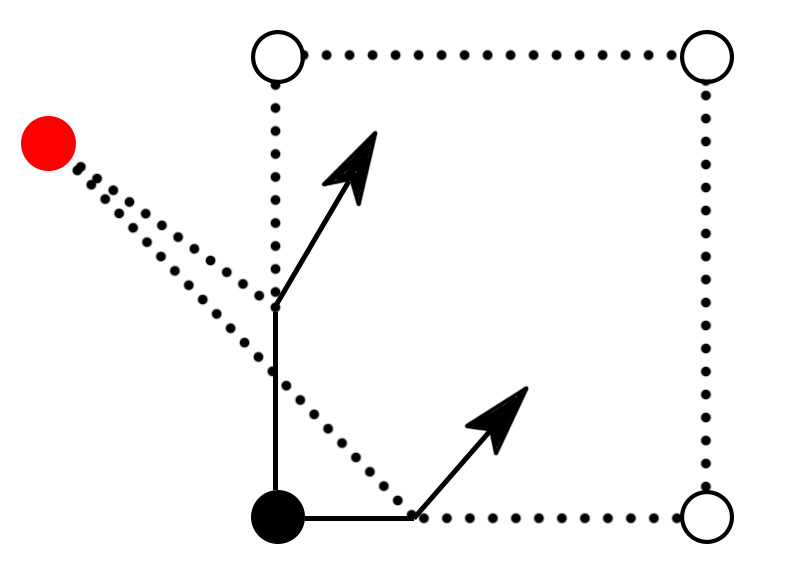
\includegraphics[width=0.4\textwidth]{Figures/DC-colinear.jpg}
    \decoRule
    \caption{Illustration of the challenge of parallel normals, leading to a QEF minimizer point outside the cell.}(\cite{Boristhebrave_2018})
    \label{fig:DC-colinear}
\end{figure}

\item \textbf{Computational Complexity:} Solving the QEF can be computationally intensive, especially for large datasets. This complexity can introduce latency in real-time applications, making it imperative to optimize the QEF minimization process.

\item \textbf{Accuracy and Precision:} Ensuring that the QEF minimizer point accurately represents the underlying data is crucial. However, noise in the data or inaccuracies in the sampling process can skew the QEF results, leading to suboptimal vertex positions.
\end{itemize}

\section{Approach for Handling Challenges in QEF Minimization}
The Quadratic Error Function minimization process involves several steps, each with its challenges and considerations. This section breaks down each step in detail to provide a comprehensive understanding of the algorithm, elucidating the underlying logic and computational methods. Figure \ref{fig:QEF-Flowchart} presents a flowchart that outlines the algorithmic steps for QEF minimization. The subsequent subsections delve into each step, providing code snippets and detailed explanations to clarify the approach.
\begin{figure}
    \centering
    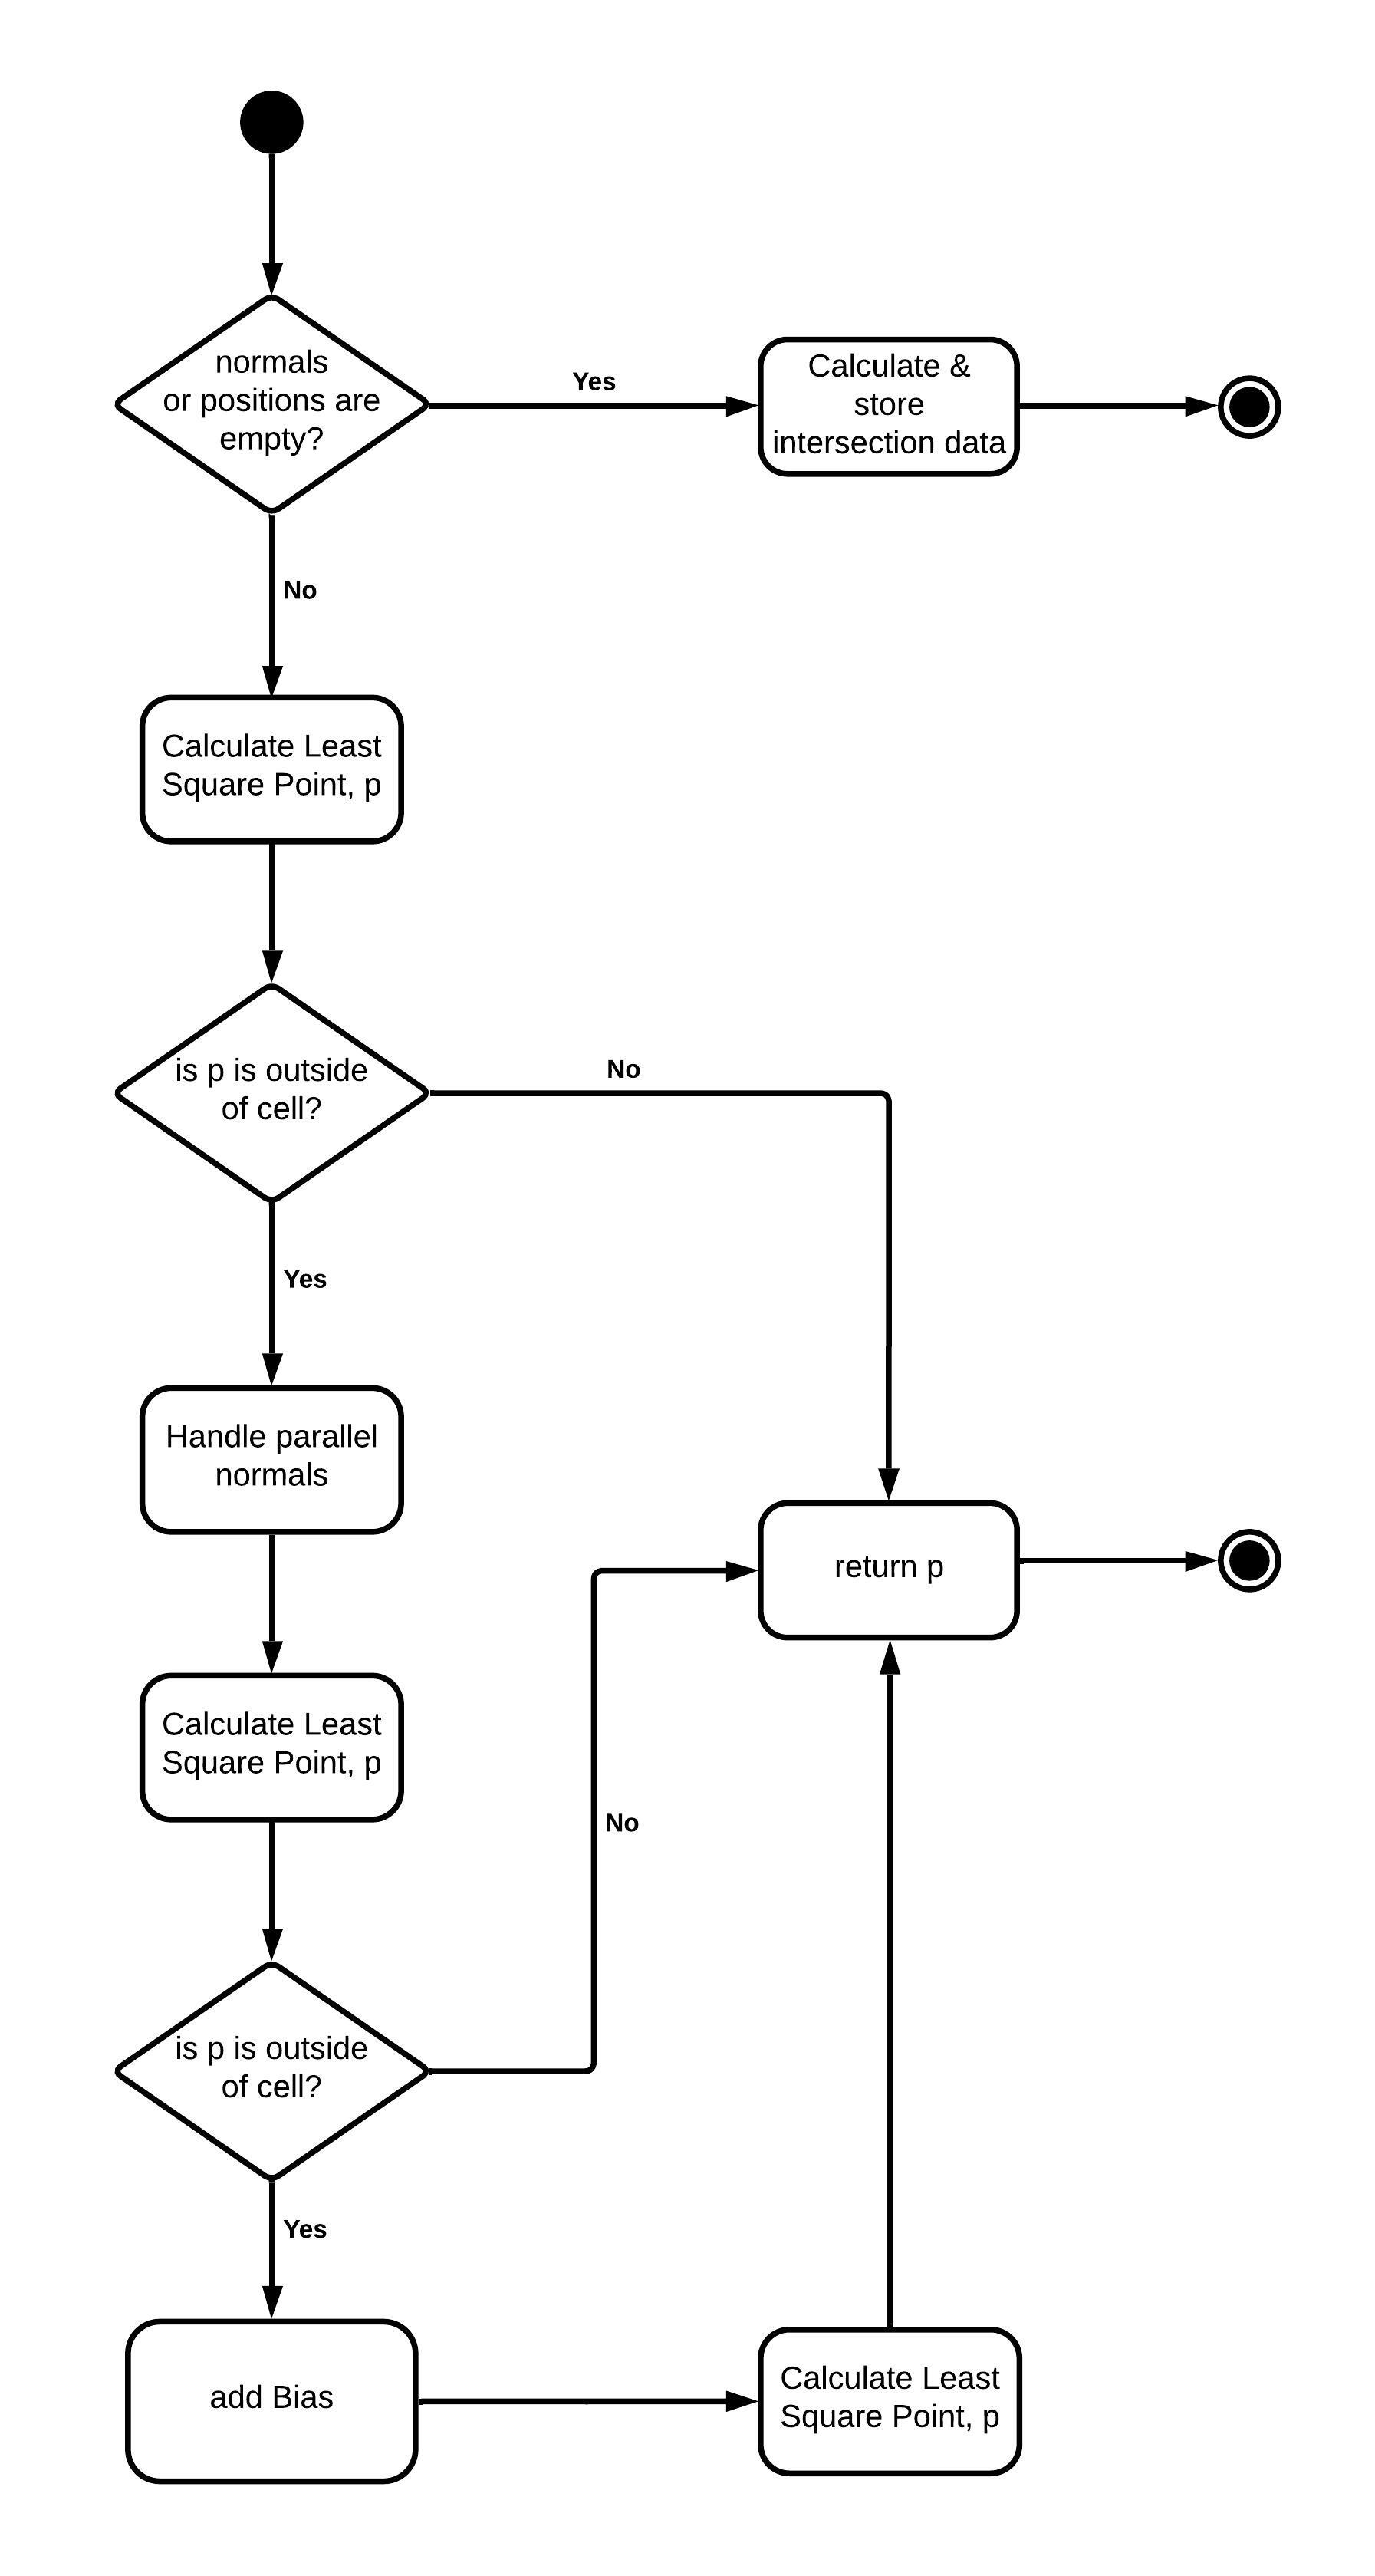
\includegraphics[width=0.83\textwidth]{Figures/QEF-FlowChart.jpeg}
    \decoRule
    \caption{Flowchart illustrating the algorithmic steps involved in QEF minimization for optimal vertex positioning within a cell.}
    \label{fig:QEF-Flowchart}
\end{figure}

\subsection{Check for Empty Normals or Positions}
The algorithm starts by checking if the input vectors for normals or positions are empty. If either is empty, the function returns a zero vector (Listing \ref{lst:isEmpty}).

\vspace{2mm}
\begin{lstlisting}[language=C++, caption=Checking for empty normals or positions, label=lst:isEmpty]
if (normals.empty() || positions.empty())
{
    displayMessage("Invalid data input for QEF calculation. Check your data.\n\n");
    return vector3();  // Return zero vector
}
\end{lstlisting}

\subsection{Initial Least Square Point Calculation}
If the normals and positions are not empty, the algorithm proceeds to calculate the least square point \( p \) using the Tikhonov regularization parameter \( \alpha \) (Listing \ref{lst:callLeastSquarePoint}).

\vspace{2mm}
\begin{lstlisting}[language=C++, caption=Initial least square point calculation, label=lst:callLeastSquarePoint]
// Tikhonov regularization parameter
double alpha = 0.1;

// Calculate the least square point using the previously explained getLeastSquarePoint function (See Listing 5.1)
vector3 p = getLeastSquarePoint(normals, positions, averagePoint, alpha);
\end{lstlisting}

\subsection{Check if Point is Outside the Cell}
The algorithm then checks if the calculated point \( p \) lies outside the cell boundaries using the `isPointOutsideCell` function (Listing \ref{lst:isPointOutside}).

\vspace{2mm}
\begin{lstlisting}[language=C++, caption=Checking if point is outside the cell, label=lst:isPointOutside]
// Check if the point is outside the cell boundaries
bool isPointOutsideCell(const vector3& p, const vector3& cellMinPoint, const vector3& cellMaxPoint)
{
    // Compare the X, Y, and Z coordinates of the point with the minimum and maximum coordinates of the cell
    // A small epsilon (1e-4) is used for tolerance
    return (p.getX() < (cellMinPoint.getX() - 1e-4)) || (point.getX() > (cellMaxPoint.getX() + 1e-4))
        || (p.getY() < (cellMinPoint.getY() - 1e-4)) || (point.getY() > (cellMaxPoint.getY() + 1e-4))
        || (p.getZ() < (cellMinPoint.getZ() - 1e-4)) || (point.getZ() > (cellMaxPoint.getZ() + 1e-4));
}
if (isPointOutside)
{
    // Handle parallel normals in the next step
}
\end{lstlisting}

\subsection{Handling Parallel Normals}
One of the challenges in QEF minimization is the presence of parallel or nearly parallel normals. These can lead to a QEF minimizer point that lies outside the cell. To address this issue, a specialized approach is adopted to detect parallel normals and adjust the QEF calculation accordingly.

The following C++ code snippet \ref{lst:handleParallelNormals} demonstrates the logic for detecting and handling parallel normals:

\vspace{2mm}
\begin{lstlisting}[language=C++, caption=Logic for detecting and handling parallel normals, label=lst:handleParallelNormals]
// Handle parallel or nearly parallel normals and average them
void handleParallelNormals(const std::vector<vector3>& normals, const std::vector<vector3>& positions, std::vector<vector3>& averagedNormals, std::vector<vector3>& averagedPositions)
{
    // Threshold for considering normals as parallel
    const double parallelThreshold = 1e-2;  
    
    // Keep track of which normals have been processed
    std::vector<bool> used(normals.size(), false);  

    // Loop through all normals
    for (int i = 0; i < normals.size(); ++i)
    {
        // Skip if this normal has already been processed
        if (used[i]) continue;  

        vector3 sumNormals = normals[i];
        vector3 sumPositions = positions[i];
        int count = 1;

        // Check for parallel normals
        for (int j = i + 1; j < normals.size(); ++j)
        {
            double dotProduct = normals[i].dot(normals[j]);
            if (!used[j] && dotProduct > (1.0 - parallelThreshold))
            {
                sumNormals = sumNormals + normals[j];
                sumPositions = sumPositions + positions[j];
                count++;
                used[j] = true;
            }
        }

        // Average the parallel normals and positions
        sumNormals.normalize();
        sumPositions /= static_cast<float>(count);

        averagedNormals.push_back(sumNormals);
        averagedPositions.push_back(sumPositions);
    }
}
\end{lstlisting}

In this code, the variable \texttt{parallelThreshold} defines how close the dot product of two normals must be to consider them parallel. The normals are considered parallel if the dot product is greater than \(1.0 - \texttt{parallelThreshold}\). This thresholding is pivotal in determining the alignment of normals. Once identified as parallel, the normals and positions are averaged. This averaging process is foundational in refining the Quadratic Error Function representation. As illustrated in Fig. \ref{fig:QEF-Handling-parallel-normals}, the initial position of the point, before averaging, might not be the optimal solution to the QEF, leading to potential inaccuracies in the surface representation.

However, after the averaging process, the QEF is recalculated. This results in a new point that, as depicted in the figure, is now inside the cell. This new QEF solution point is more representative of the underlying surface, ensuring a closer alignment with the actual data. It's a testament to the power of the averaging process, which not only refines the position of the point but also optimizes the QEF solution, leading to a more accurate and robust surface representation.


\begin{figure}
\centering
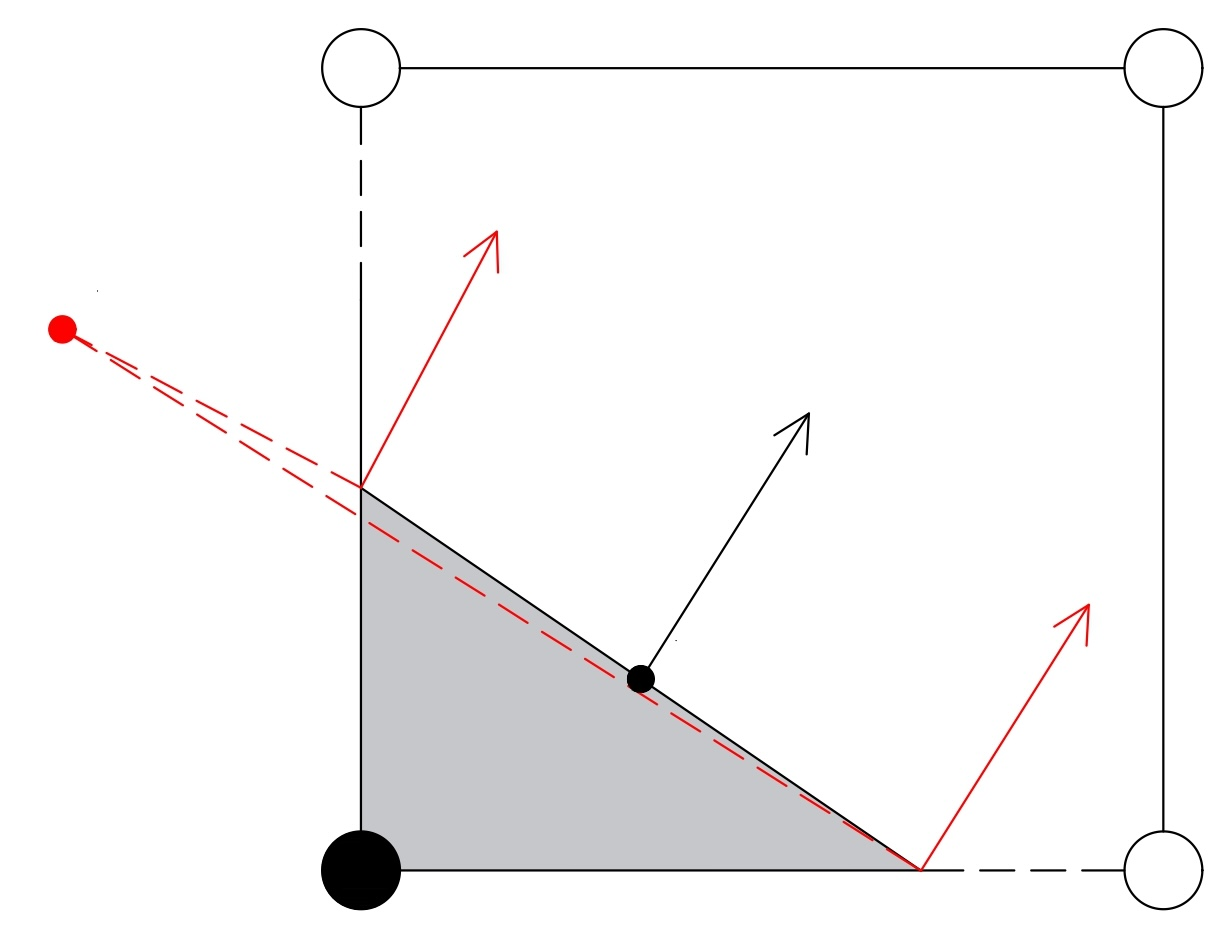
\includegraphics[width=0.6\textwidth]{Figures/aveg-parallal-normals.jpg}
\decoRule
\caption{Illustration of the QEF point refinement process. The red arrows indicate the original normals, representing the initial orientations before refinement. The red point denotes the original QEF solution without handling parallel normals. After addressing and averaging parallel normals, the QEF point is recalculated and represented by the black point. This figure underscores the significance of handling parallel normals in achieving a more accurate surface representation.}
\label{fig:QEF-Handling-parallel-normals}
\end{figure}

\subsection{Adding Bias to Pull Point Towards Cell Center}
If the point \( p \) still lies outside the cell boundaries after handling parallel normals, a bias is added at the center of the cell to pull the QEF point towards the center. This is done by adding additional normals and positions to the averaged list (Listing \ref{lst:addBias}).

\vspace{2mm}
\begin{lstlisting}[language=C++, caption=Adding bias to pull point towards cell center, label=lst:addBias]
// Add bias normals and positions to pull the point towards the cell center
vector3 biasNormalX(0.1, 0.0, 0.0);
vector3 biasNormalY(0.0, 0.1, 0.0);
vector3 biasNormalZ(0.0, 0.0, 0.1);

averagedNormals.push_back(biasNormalX);
averagedNormals.push_back(biasNormalY);
averagedNormals.push_back(biasNormalZ);

averagedPositions.push_back(averagePoint);
averagedPositions.push_back(averagePoint);
averagedPositions.push_back(averagePoint);

// Recalculate the least square point after adding bias
p = getLeastSquarePoint(averagedNormals, averagedPositions, averagePoint, alpha);
\end{lstlisting}

\subsection{Final Check and Clamping the Point}

After adding the bias, the algorithm checks again if the point \( p \) lies outside the cell boundaries. If it does, the point is clamped to the nearest edge of the cell using the \texttt{clamp} function (Listing \ref{lst:clamping}).

\vspace{2mm}
\begin{lstlisting}[language=C++, caption=Final check and clamping the point to the nearest boundary, label=lst:clamping]
// Final check for point outside the cell boundaries
bool isPointOutsideAfterBias = isPointOutsideCell(point, cellMinPoint, cellMaxPoint);

if (isPointOutsideAfterBias)
{
    p.setX(clamp(point.getX(), cellMinPoint.getX(), cellMaxPoint.getX()));
    p.setY(clamp(point.getY(), cellMinPoint.getY(), cellMaxPoint.getY()));
    p.setZ(clamp(point.getZ(), cellMinPoint.getZ(), cellMaxPoint.getZ()));
}
\end{lstlisting}

\subsubsection{Implications of Clamping on Geometric Representation}

The clamping process, while ensuring that the QEF minimizer point lies within the cell, can introduce some geometric artifacts. Specifically, clamping can lead to:

\begin{enumerate}
    \item \textbf{Loss of Surface Smoothness}: When the QEF minimizer point is clamped to the nearest cell boundary, it can disrupt the continuity of the surface, leading to potential sharp edges or corners. This is especially noticeable when multiple adjacent cells have their minimizer points clamped, resulting in a visible discontinuity in the isosurface.
    
    \item \textbf{Deviation from True Surface}: The clamped point might not be the true minimizer of the QEF. As a result, the generated isosurface might deviate from the actual underlying data. This deviation can lead to inaccuracies in the geometric representation, especially in regions with complex surface features.
    
    \item \textbf{Bias towards Cell Boundaries}: The clamping process can introduce a bias where the isosurface tends to adhere more closely to cell boundaries, especially in areas with sparse or ambiguous data. This can lead to an over-representation of the cell grid structure on the final surface.
\end{enumerate}

To address these potential issues, it's essential to strike a balance between ensuring the QEF minimizer point lies within the cell and preserving the integrity of the geometric representation. Some potential solutions include:

\begin{enumerate}
    \item \textbf{Adaptive Cell Sizing with Octree Implementation}: Leveraging octree data structures can facilitate adaptive cell sizing based on the density or complexity of the data. In regions with intricate surface features, the octree can subdivide cells to create smaller cells, leading to a more accurate QEF solution and reducing the need for clamping. The hierarchical nature of the octree ensures efficient spatial subdivision, allowing for finer granularity where needed while maintaining larger cells in less complex regions.
    
    \item \textbf{Post-Processing Smoothing}: After the isosurface generation, a post-processing step can be applied to smooth out the surface, especially in regions affected by clamping. This can help in restoring some of the surface continuity.
\end{enumerate}

\noindent In essence, while clamping offers a practical solution, it's vital to understand its geometric implications and employ strategies to address them for a more accurate isosurface representation. The algorithm effectively handles various challenges in QEF minimization, including empty normals, parallel normals, and points outside the cell boundaries. By adding a bias towards the cell center, the algorithm ensures that the QEF minimizer point is more likely to lie within the cell, thereby improving the accuracy of the generated isosurface.

\section{Code Deployment} 
GitHub (\cite{github}) is a popular desktop and web hosting platform for Continuous Integration (CI) and Continuous Deployment (CD) of software code. The code base of the Simulation Platform is developed on Visual Studio code IDE (Integrated Development Environment). The entire code base and the results of this thesis work are deployed to GitHub and can be viewed via link \url{https://github.com/pth68/SimulationPlatform}.

\section{Summary}
This chapter provided a deep dive into the Quadratic Error Function and its pivotal role in Dual Contouring and Dual Marching Cubes algorithms. The chapter began with simplifying the QEF equation, making it more accessible, and setting the stage for its practical implementation.

The Eigen C++ library emerged as a powerful ally in this journey, enabling efficient and accurate linear algebra operations. The chapter presented a comprehensive algorithmic flow for QEF calculation, addressing challenges such as handling colinear normals and ensuring the calculated point remains within the cell boundaries.

Special attention was given to the challenges in QEF minimization. Strategies like averaging parallel normals and adding a bias towards the cell center were introduced to address potential pitfalls. The chapter also provided a detailed breakdown of the algorithm's steps, from initial checks to the final clamping of the point.

In essence, Chapter \ref{Chapter5} served as a deep dive into the QEF methodology, offering a mix of theory, practical challenges, and coding insights. With a robust understanding of the QEF and its intricacies, readers are well-equipped to tackle the challenges of isosurface extraction. With a solid understanding of QEF methodology and its challenges, the stage is set for us to delve into the practical implementation of the Dual Contouring and Dual Marching Cubes algorithms, which will be the focus of the next chapter.

% \section{Summary}
% This chapter provides a comprehensive overview of the Quadratic Error Function and its application in isosurface extraction, specifically in the context of Dual Contouring and Dual Marching Cubes algorithms. The chapter begins by simplifying the QEF equation and introducing a matrix formulation that is numerically stable and robust, thanks to the application of Singular Value Decomposition and Tikhonov regularization.

% The Eigen C++ library is introduced as a powerful tool for performing the required linear algebra operations efficiently. An algorithmic flow for QEF calculation is presented, complete with a C++ implementation that leverages Eigen's capabilities. The algorithm addresses challenges such as handling colinear normals, computational complexity, and ensuring accuracy and precision.

% Special attention is given to the challenges in QEF minimization, including handling parallel or nearly parallel normals, which can cause the QEF minimizer point to lie outside the cell. The algorithm incorporates checks and balances at multiple stages to ensure the calculated point is within the cell boundaries. If the point lies outside, the algorithm employs strategies like averaging parallel normals and adding a bias towards the cell center to pull the point back into the cell.

% The chapter concludes with a detailed algorithmic flow, breaking down each step involved in QEF minimization. This includes initial checks for empty data, least square point calculation, and specialized handling for parallel normals and points outside the cell.

% Overall, this chapter serves as a comprehensive guide for anyone looking to understand or implement QEF minimization in the context of isosurface extraction. It offers a balanced mix of theory, practical challenges, and coding insights, making it a valuable resource for researchers and practitioners. With a solid understanding of QEF methodology and its challenges, the stage is set for us to delve into the practical implementation of the Dual Contouring and Dual Marching Cubes algorithms, which will be the focus of the next chapter.
\chapter{Implementation and Results of Dual Contouring and Dual Marching Cubes Algorithms} \label{Chapter6}

This chapter aims to provide a comprehensive overview of the implementation details and results obtained from applying the Dual Contouring (DC) and Dual Marching Cubes (DMC) algorithms for isosurface extraction. Building upon the theoretical foundations laid out in Chapter \ref{Chapter3}, the fundamental data structures introduced in Chapter \ref{Chapter4}, and the Quadratic Error Function methodology discussed in \ref{Chapter5}, this chapter will delve into the practical aspects of these algorithms. It will cover code snippets, mesh generation, and visual results, offering a holistic view of how DC and DMC can be effectively implemented and what kind of results one can expect.

\section{Dual Contouring Algorithm Overview}
In this section, we revisit the Dual Contouring algorithm, which was extensively discussed in Section \ref{Dual-Contouring}. The focus here is to lay the groundwork for the forthcoming implementation details. As a quick recap, Dual Contouring is particularly effective for preserving sharp features and handling complex topologies. 

\subsection{Implementation Steps}

The algorithm operates through a series of steps, from initializing the regular grid to solving the Quadratic Error Function for optimal point placement within grid cells. The subsequent sections will delve into the practical aspects of implementing these steps, supported by code snippets for clarity. Figure \ref{fig:dc-flow-chart} illustrates the flow diagram for the Dual Contouring algorithm. This flow diagram serves as a roadmap for the implementation, guiding the reader through the sequence of operations that transform raw data into a refined mesh. By the end of this section, the reader will clearly understand how each theoretical component from Section \ref{Dual-Contouring} translates into practical code.

\begin{figure}[H]
\centering
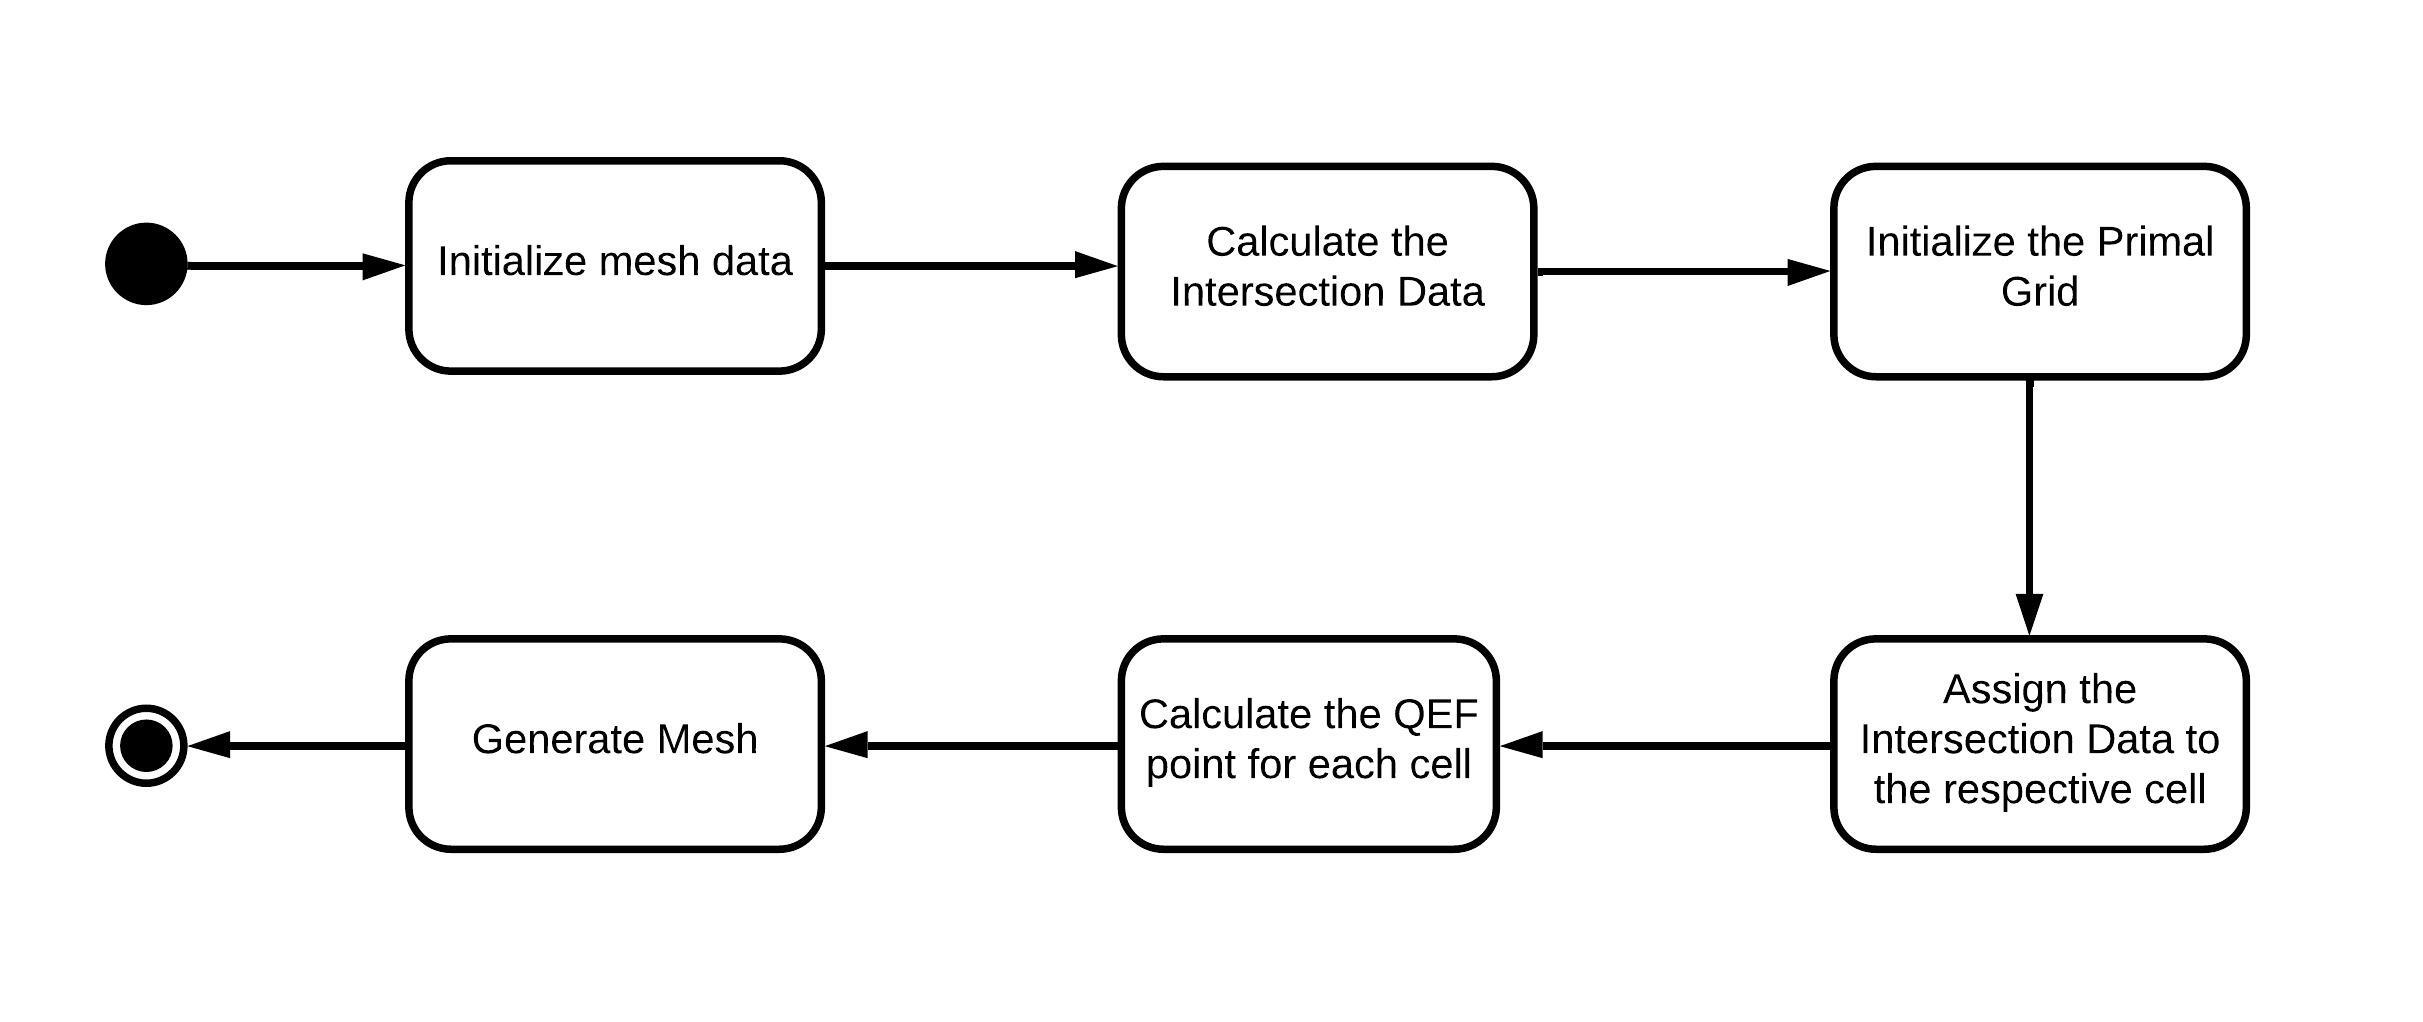
\includegraphics[width=1.0\textwidth]{Figures/DC-FlowChart.jpeg}
\decoRule
\caption{Flow chart for implementation of DC algorithm}
\label{fig:dc-flow-chart}
\end{figure}

\subsubsection{Initializing Mesh Data}

The first step in the Dual Contouring algorithm is to initialize the mesh data. This involves setting up the mesh lines along the X, Y, and Z axes. These mesh lines are crucial for firing rays in the subsequent steps and defining the primal grid where the algorithm will operate. For a more detailed explanation of what mesh lines and padded mesh lines are, refer back to Section \ref{meshLines} in Chapter \ref{Chapter4}. Here is a snippet of code (Listing \ref{lst:meshLines}) that initializes the mesh lines.

\vspace{2mm}
\begin{lstlisting}[language=C++, caption=Initializing Mesh Data, label=lst:meshLines]
std::vector<double> meshLinesX = meshData->getMeshLinesX();
std::vector<double> meshLinesY = meshData->getMeshLinesY();
std::vector<double> meshLinesZ = meshData->getMeshLinesZ();
\end{lstlisting}

The code snippet in Listing \ref{lst:meshLines} retrieves the mesh lines along the X, Y, and Z axes from a pre-populated \texttt{meshData} object. The vectors \texttt{meshLinesX}, \texttt{meshLinesY}, and \texttt{meshLinesZ} will hold the mesh lines for each respective axis. 

\subsubsection{Calculate the Intersection Data}

After initializing the mesh data, the next step is to calculate the intersection data, and for that, Intel Embree API is used. This is a crucial step for calculating and storing intersection data, which will be used later for mesh generation. The ray-casting process is detailed in Section \ref{ray-casting} of Chapter \ref{Chapter4}. Here is a snippet of code that fires rays along the mesh lines:

\begin{lstlisting}[language=C++, caption=Firing Rays Along Mesh Lines]
fireRaysAlongMeshLines(meshData);
\end{lstlisting}

The function \texttt{fireRaysAlongMeshLines} (as illustrated in Listing \ref{lst:fireRaysAlongMeshLines}) takes the pre-populated \texttt{meshData} object as an argument. This function is responsible for firing rays along the mesh lines stored in \texttt{meshData} and updating the intersection data accordingly.

\subsubsection{Initializing the Primal Grid}

The primal grid is a foundational structure in the Dual Contouring algorithm, serving as the primary framework for storing intersection data. This grid is essentially a three-dimensional structure, where each cell is an instance of the \texttt{PrimalGridCell} structure. The dimensions of this grid are determined by the sizes of the \texttt{meshLinesX}, \texttt{meshLinesY}, and \texttt{meshLinesZ} vectors, which represent the mesh lines in each respective direction.

\begin{lstlisting}[language=C++, caption=Initializing the Primal Grid, label=lst:Init-Primal-Grid]
std::vector<std::vector<std::vector<PrimalGridCell>>> primalGrid(meshLinesX.size() - 1,
    std::vector<std::vector<PrimalGridCell>>(meshLinesY.size() - 1, std::vector<PrimalGridCell>(meshLinesZ.size() - 1)));
\end{lstlisting}

The code snippet \ref{lst:Init-Primal-Grid} shows how the primal grid is initialized as a three-dimensional vector of \texttt{PrimalGridCell} structures. For a comprehensive understanding of the structure and functionality of the \texttt{PrimalGridCell} and the primal grid's significance in the context of the Dual Contouring algorithm, readers are referred to Section \ref{Data-Structures}, specifically Subsections \ref{PrimalGridCell} and \ref{Primal-Grid-Mesh} of Chapter \ref{Chapter4}.

\subsubsection{Assign Intersection Data to Respective Cell}

Once the primal grid is initialized, the next step is to populate each cell with the intersection data. This involves iterating over each cell in the grid and checking if any intersection points fall within its boundaries. If they do, these points and their corresponding normals are stored in the cell.

\begin{lstlisting}[language=C++, caption=Assigning intersection data to the primal grid cells, label=lst:sort-intersection-data]
for (int i = 0; i < meshLinesX.size() - 1; i++)
{
    for (int j = 0; j < meshLinesY.size() - 1; j++)
    {
        for (int k = 0; k < meshLinesZ.size() - 1; k++)
        {
            PrimalGridCell primalCell;

            // Define the boundaries of the current cell
            double x1 = meshLinesX[i], x2 = meshLinesX[i + 1];
            double y1 = meshLinesY[j], y2 = meshLinesY[j + 1];
            double z1 = meshLinesZ[k], z2 = meshLinesZ[k + 1];

            vector3 cellMinPoint(x1, y1, z1);
            vector3 cellMaxPoint(x2, y2, z2);

            primalCell.cellMinPoint = cellMinPoint;
            primalCell.cellMaxPoint = cellMaxPoint;

            // Check each intersection point to see if it lies within the current cell
            for (int h = 0; h < intersectionData.hitPoints.size(); h++)
            {
                vector3 hitPoint = intersectionData.hitPoints[h];
                vector3 hitNormal = intersectionData.hitNormals[h];

                if (hitPoint.isWithinBounds(cellMinPoint, cellMaxPoint, tol))
                {
                    primalCell.hitPoints.push_back(hitPoint);
                    primalCell.hitNormals.push_back(hitNormal);
                    primalCell.averagePoint += hitPoint;
                }
            }

            // If the cell contains intersection points, calculate the average and QEF point
            if (!primalCell.hitPoints.empty())
            {
                primalCell.averagePoint /= primalCell.hitPoints.size();
                primalCell.QEFPoint = calculateQEF(primalCell.hitNormals, primalCell.hitPoints, primalCell.averagePoint, primalCell.cellMinPoint, primalCell.cellMaxPoint);

            }
            else
            {
                primalCell.averagePoint = (cellMinPoint + cellMaxPoint) / 2;
            }

            primalGrid[i][j][k] = primalCell;
        }
    }
}
\end{lstlisting}

In the Listing \ref{lst:sort-intersection-data}, the nested loops iterate over each cell in the primal grid. For each cell, the boundaries are defined using the mesh lines. Then, each intersection point is checked to determine if it lies within the current cell's boundaries. If it does, the point and its corresponding normal are stored in the cell. After all intersection points have been checked for a particular cell, the average point and QEF point for the cell are calculated if the cell contains any intersection points. If the cell doesn't have any intersection points, the average point is set to the midpoint of the cell. Finally, the populated \texttt{PrimalGridCell} is assigned to its respective position in the primal grid. For a deeper understanding of the structures and functions used, readers are referred to Section \ref{Data-Structures} of Chapter \ref{Chapter4}.

\subsubsection{Calculate QEF}

The QEF is a pivotal component in the Dual Contouring algorithm, responsible for determining the optimal vertex position within a grid cell. In the previous step, the QEF was computed for cells containing intersection points using the \texttt{calculateQEF} function while assigning intersection data to each cell.

For an in-depth understanding of the QEF calculation, revisiting the comprehensive discussion in Chapter \ref{Chapter5} is recommended. In the context of this chapter, it is essential to grasp that the QEF provides a measure of error for a given vertex position within a cell. By minimizing this error, the algorithm ensures that the vertex position best represents the underlying scalar field, leading to a high-quality mesh representation.

\subsubsection{Mesh Generation}

With the intersection data assigned to the respective cells and the QEF points calculated, the last step for the Dual Contouring algorithm is to generate the mesh. This involves connecting the QEF points of adjacent cells to form the mesh triangles. Figure \ref{fig:DC-cube} provides a visual representation of this process, showcasing a cube and its corresponding mesh generated using the Dual Contouring algorithm.

\begin{figure}[H]
    \centering
    \begin{subfigure}{0.5\textwidth}
        \centering
        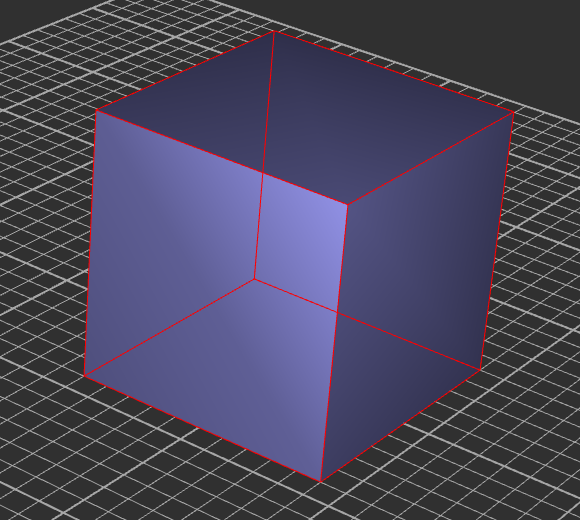
\includegraphics[height=0.7\textwidth, width=0.85\linewidth]{Figures/cube0.png}
    \end{subfigure}%
    \begin{subfigure}{0.5\textwidth}
        \centering
        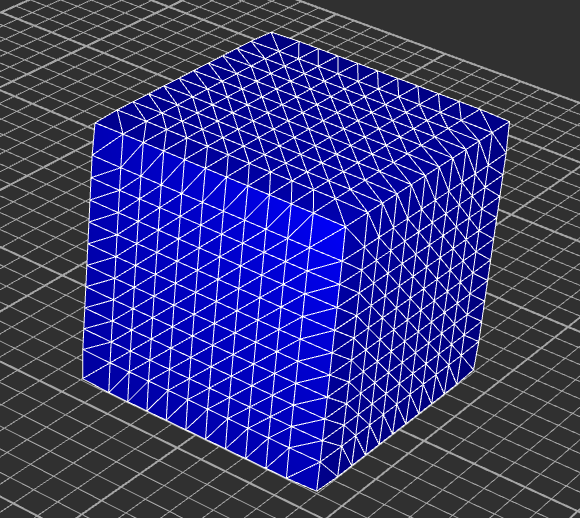
\includegraphics[height=0.7\textwidth, width=0.85\linewidth]{Figures/cube0-DC.png}
    \end{subfigure}
    \decoRule
    \caption{Cube and its mesh representation generated by the Dual Contouring algorithm.}
    \label{fig:DC-cube}
\end{figure}

In Listing \ref{lst:meshGeneration}, the code responsible for mesh generation is presented. For each cell in the primal grid, if the cell contains intersection points, the QEF point of the cell is connected with the QEF points of its adjacent cells in the positive x, y, and z directions. This algorithmic approach forms the triangles of the mesh, ensuring a coherent and accurate representation of the surface.

\vspace{2mm}
\begin{lstlisting}[language=C++, caption=Mesh Generation Using QEF Points, label=lst:meshGeneration]
for (int i = 0; i < meshLinesX.size() - 1; i++)
{
	for (int j = 0; j < meshLinesY.size() - 1; j++)
	{
		for (int k = 0; k < meshLinesZ.size() - 1; k++)
		{
			PrimalGridCell& cell = primalGrid[i][j][k];

			if (!cell.hitPoints.empty())
			{
				vector3& QEFPoint = cell.QEFPoint;

				// Connect to the cell in positive x direction
				if (i + 1 < meshLinesX.size() - 1 &&
					j + 1 < meshLinesY.size() - 1 &&
					!primalGrid[i + 1][j][k].hitPoints.empty() &&
					!primalGrid[i + 1][j + 1][k].hitPoints.empty() &&
					!primalGrid[i][j + 1][k].hitPoints.empty())
				{
					vector3& adjacentCentroidX = primalGrid[i + 1][j][k].QEFPoint;
					vector3& adjacentCentroidY = primalGrid[i][j + 1][k].QEFPoint;
					vector3& adjacentCentroidXY = primalGrid[i + 1][j + 1][k].QEFPoint;

					annotationTikhonovRegularization->addTriangle(QEFPoint.getX(), QEFPoint.getY(), QEFPoint.getZ(),
						adjacentCentroidX.getX(), adjacentCentroidX.getY(), adjacentCentroidX.getZ(),
						adjacentCentroidXY.getX(), adjacentCentroidXY.getY(), adjacentCentroidXY.getZ(), 0.0, 0.0, 0.6);

					annotationTikhonovRegularization->addTriangle(QEFPoint.getX(), QEFPoint.getY(), QEFPoint.getZ(),
						adjacentCentroidY.getX(), adjacentCentroidY.getY(), adjacentCentroidY.getZ(),
						adjacentCentroidXY.getX(), adjacentCentroidXY.getY(), adjacentCentroidXY.getZ(), 0.0, 0.0, 0.6);
				}

				// Connect to the cell in positive y direction
				if (j + 1 < meshLinesY.size() - 1 &&
					k + 1 < meshLinesZ.size() - 1 &&
					!primalGrid[i][j + 1][k].hitPoints.empty() &&
					!primalGrid[i][j][k + 1].hitPoints.empty() &&
					!primalGrid[i][j + 1][k + 1].hitPoints.empty())
				{
					vector3& adjacentCentroidY = primalGrid[i][j + 1][k].QEFPoint;
					vector3& adjacentCentroidZ = primalGrid[i][j][k + 1].QEFPoint;
					vector3& adjacentCentroidYZ = primalGrid[i][j + 1][k + 1].QEFPoint;

					annotationTikhonovRegularization->addTriangle(QEFPoint.getX(), QEFPoint.getY(), QEFPoint.getZ(),
						adjacentCentroidY.getX(), adjacentCentroidY.getY(), adjacentCentroidY.getZ(),
						adjacentCentroidYZ.getX(), adjacentCentroidYZ.getY(), adjacentCentroidYZ.getZ(), 0.0, 0.0, 0.6);

					annotationTikhonovRegularization->addTriangle(QEFPoint.getX(), QEFPoint.getY(), QEFPoint.getZ(),
						adjacentCentroidZ.getX(), adjacentCentroidZ.getY(), adjacentCentroidZ.getZ(),
						adjacentCentroidYZ.getX(), adjacentCentroidYZ.getY(), adjacentCentroidYZ.getZ(), 0.0, 0.0, 0.6);
				}

				// Connect to the cell in positive z direction
				if (k + 1 < meshLinesZ.size() - 1 &&
					i + 1 < meshLinesX.size() - 1 &&
					!primalGrid[i][j][k + 1].hitPoints.empty() &&
					!primalGrid[i + 1][j][k].hitPoints.empty() &&
					!primalGrid[i + 1][j][k + 1].hitPoints.empty())
				{
					vector3& adjacentCentroidZ = primalGrid[i][j][k + 1].QEFPoint;
					vector3& adjacentCentroidX = primalGrid[i + 1][j][k].QEFPoint;
					vector3& adjacentCentroidXZ = primalGrid[i + 1][j][k + 1].QEFPoint;

					annotationTikhonovRegularization->addTriangle(QEFPoint.getX(), QEFPoint.getY(), QEFPoint.getZ(),
						adjacentCentroidZ.getX(), adjacentCentroidZ.getY(), adjacentCentroidZ.getZ(),
						adjacentCentroidXZ.getX(), adjacentCentroidXZ.getY(), adjacentCentroidXZ.getZ(), 0.0, 0.0, 0.6);

					annotationTikhonovRegularization->addTriangle(QEFPoint.getX(), QEFPoint.getY(), QEFPoint.getZ(),
						adjacentCentroidX.getX(), adjacentCentroidX.getY(), adjacentCentroidX.getZ(),
						adjacentCentroidXZ.getX(), adjacentCentroidXZ.getY(), adjacentCentroidXZ.getZ(), 0.0, 0.0, 0.6);
				}
			}
		}
	}
}
\end{lstlisting}
\vspace{2mm}

In the mesh generation process, while the ideal representation for connecting the QEF points would be quads, due to technical constraints, triangles are used instead. When converting a quadrilateral into triangles, there are multiple ways to split it. In this implementation, the QEF point of a cell is connected with the QEF points of its adjacent cells in the positive x, y, and z directions. For each connection direction, two triangles are formed to represent the surface of the quadrilateral. For instance, when connecting in the positive x direction, one triangle is formed using the QEF point, the adjacent QEF point in the x direction, and the QEF point in the combined x-y direction. A second triangle is then formed using the QEF point, the adjacent QEF point in the y direction, and the QEF point in the combined x-y direction. This methodical approach ensures that the resulting triangles accurately represent the underlying surface and maintain the integrity of the mesh.

\section{Dual Marching Cubes Implementation} \label{sec:dmc-implementation}

In this section, we revisit the Dual Marching Cubes algorithm, comprehensively explored in Section \ref{Dual-Marching-Cubes} of Chapter \ref{Chapter3}. The primary focus here is to bridge the gap between the theoretical underpinnings and the practical implementation of the algorithm. To briefly recap, the Dual Marching Cubes algorithm is renowned for generating adaptive, topologically accurate meshes that faithfully reproduce thin features, marking it as a significant advancement in isosurface extraction.

\subsection{Algorithm Overview}

The Dual Marching Cubes algorithm builds upon the robustness of Marching Cubes and the adaptability of Dual Contouring, aiming to produce detailed and topologically sound meshes. It operates through a sequence of steps, from constructing a dual grid to refining the generated mesh using Quadratic Error Function calculations. The following sections provide a detailed walkthrough of these steps, accompanied by code snippets for a clearer understanding. Figure \ref{fig:dmc-flow-chart} presents a flow diagram to guide the reader through the DMC algorithm's implementation process. This diagram serves as a roadmap, elucidating how each theoretical concept from Section \ref{Dual-Marching-Cubes} is translated into actionable code.

While sharing some similarities with Dual Contouring, the Dual Marching Cubes algorithm introduces unique steps that focus on the dual grid of the scalar field. This section provides a detailed walkthrough of the DMC implementation, divided into three main parts.

\begin{figure}[ht!]
\centering
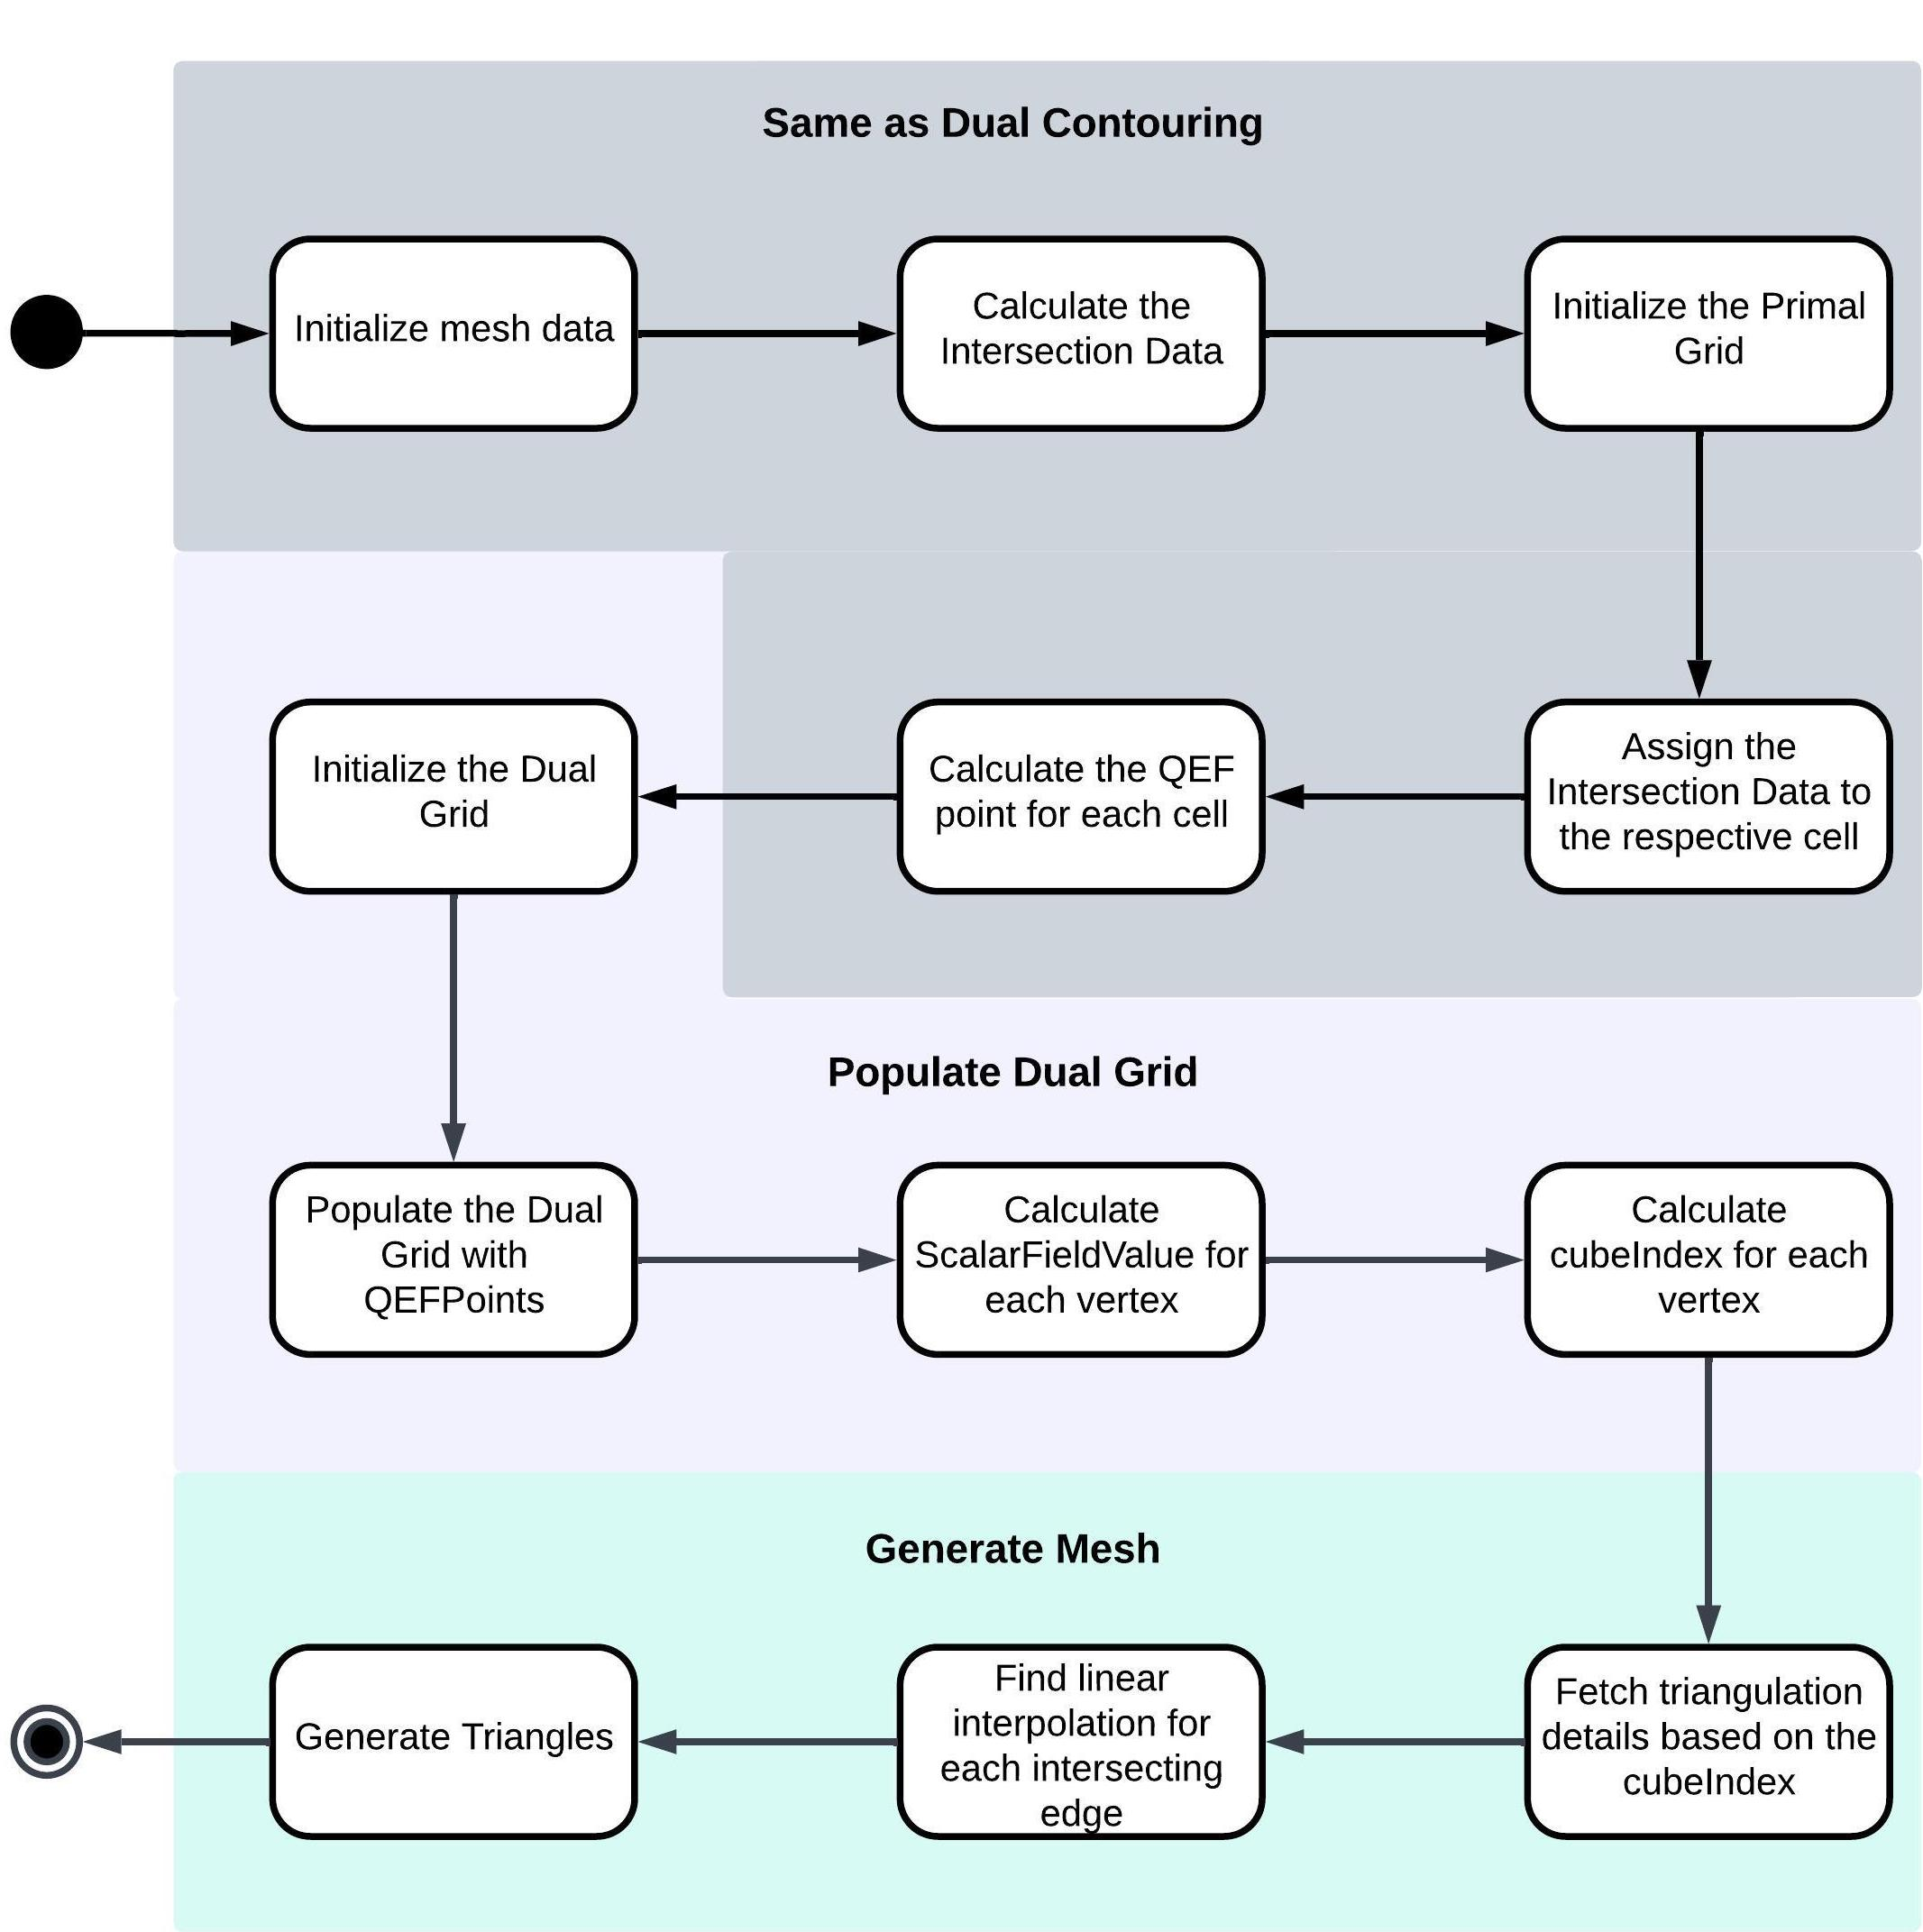
\includegraphics[width=1.0\textwidth]{Figures/DMC-FlowChart.jpeg}
\decoRule
\caption{Flow chart for implementation of DMC algorithm}
\label{fig:dmc-flow-chart}
\end{figure}

\subsection{Shared Foundations with Dual Contouring}

The initial steps of the DMC algorithm mirror those of Dual Contouring. This phase ensures that the foundational data structures and initial computations are in place, setting the stage for the unique aspects of DMC.

% Here, you can briefly mention the steps that are the same as in DC without going into the details since they were covered in the previous section.

\subsection{Populating the Dual Grid} \label{populating-dual-grid}

As the name suggests, the Dual Marching Cubes algorithm introduces a dual grid structure that complements the primal grid used in the initial stages. This dual grid is pivotal in the algorithm's ability to generate topologically accurate and feature-preserving meshes. Populating this grid is a multi-faceted process that ensures the grid is equipped with all the necessary data points and attributes required for the subsequent mesh generation phase.

This section will delve into the intricacies of initializing and populating the dual grid. This involves setting up the grid's structure, assigning values, determining scalar field values for each vertex, and calculating the cube index that will guide the triangulation process. Each of these steps is crucial in ensuring that the dual grid is primed for the final mesh generation, and we will explore them in detail in the following subsections.

\subsubsection{Initialization of the Dual Grid}

The initialization of the dual grid is a foundational step in the Dual Marching Cubes algorithm. This grid, constructed using a nested vector list, serves as the primary data structure that will hold the vertices, scalar field values, and other essential attributes required for the subsequent algorithm steps.

\vspace{2mm}
\begin{lstlisting}[language=C++, caption=Initializing the Dual Grid, label=lst:dualGridInit]
std::vector<std::vector<std::vector<DualGridCell>>> dualGrid(
    paddedMeshLinesX.size() - 1,
    std::vector<std::vector<DualGridCell>>(
        paddedMeshLinesY.size() - 1,
        std::vector<DualGridCell>(paddedMeshLinesZ.size() - 1)
    )
);
\end{lstlisting}
The code snippet in Listing \ref{lst:dualGridInit} initializes the dual grid using a 3D nested vector list. Each cell in this grid corresponds to the \texttt{DualGridCell} structure, as detailed in Section \ref{DualGridCell}. The grid's dimensions are defined by the \texttt{paddedMeshLines} across the X, Y, and Z axes, which, as mentioned in Section \ref{meshLines}, are enhanced mesh lines tailored for efficient boundary handling. This nested vector representation, highlighted in Section \ref{Dual-Grid-Mesh}, not only ensures efficient data storage and quick access but also simplifies the implementation process. Such a structure is crucial for the Dual Marching Cubes algorithm, offering a robust framework for mesh generation data processing.

\subsubsection{Populating the Dual Grid with QEF Points}
Once the dual grid is initialized, the next crucial step is to populate it with the QEF points. These points are derived from the primal grid and represent the optimal vertex positions within each cell of the dual grid.

\vspace{2mm}
\begin{lstlisting}[language=C++, caption=Populating the Dual Grid with QEF Points, label=lst:populateDualGrid]
double isovalue = 0.5;
for (int i = 0; i < paddedMeshLinesX.size() - 2; i++) {
    for (int j = 0; j < paddedMeshLinesY.size() - 2; j++) {
        for (int k = 0; k < paddedMeshLinesZ.size() - 2; k++) {
            DualGridCell& dualCell = dualGrid[i][j][k];  
    
            dualCell.vertices[0] = getVertexFromPaddedPrimalCell(i, j, k, paddedPrimalGrid);
            dualCell.vertices[1] = getVertexFromPaddedPrimalCell(i + 1, j, k, paddedPrimalGrid);
            dualCell.vertices[2] = getVertexFromPaddedPrimalCell(i + 1, j + 1, k, paddedPrimalGrid);
            dualCell.vertices[3] = getVertexFromPaddedPrimalCell(i, j + 1, k, paddedPrimalGrid);
            dualCell.vertices[4] = getVertexFromPaddedPrimalCell(i, j, k + 1, paddedPrimalGrid);
            dualCell.vertices[5] = getVertexFromPaddedPrimalCell(i + 1, j, k + 1, paddedPrimalGrid);
            dualCell.vertices[6] = getVertexFromPaddedPrimalCell(i + 1, j + 1, k + 1, paddedPrimalGrid);
            dualCell.vertices[7] = getVertexFromPaddedPrimalCell(i, j + 1, k + 1, paddedPrimalGrid);
    
            //Populate scalar field values
            for (int v = 0; v < 8; v++) {
                const vector3& vertex = dualCell.vertices[v];
                bool inside = testPointInside(vertex.getX(), vertex.getY(), vertex.getZ());
                dualCell.scalarFieldValues[v] = inside ? 1.0 : 0.0;  
    
                if (dualCell.scalarFieldValues[v] > isovalue) {
                    dualCell.cubeIndex |= 1 << v;
                }
            }
        }
    }
}
\end{lstlisting}
\vspace{2mm}

The dual grid vertices are constructed by iterating through the padded mesh lines in the above code snippet (Listing \ref{lst:populateDualGrid}). For each cell in the dual grid, the vertices are populated using the \texttt{getVertexFromPaddedPrimalCell} function, which fetches the QEF point (or centroid) from the corresponding cell in the padded primal grid.

\vspace{2mm}
\begin{lstlisting}[language=C++, caption=Fetching Vertex from Padded Primal Cell, label=lst:getVertex]
Vector3 getVertexFromPaddedPrimalCell(int i, int j, int k, const std::vector<std::vector<std::vector<PrimalGridCell>>>& paddedPrimalGrid) {
	// If coordinates are out of bounds, return an empty vector
	if (i >= paddedPrimalGrid.size() || j >= paddedPrimalGrid[0].size() || k >= paddedPrimalGrid[0][0].size()) {
		return vector3::Empty();
	}

	const PrimalGridCell& primalCell = paddedPrimalGrid[i][j][k];

	// Check if QEFPoint is set (not equal to zero vector)
	if (primalCell.QEFPoint != vector3::Empty()) {
		return primalCell.QEFPoint;
	}
	else {
		// Compute the center of the PrimalGridCell
		return (primalCell.cellMinPoint + primalCell.cellMaxPoint) / 2.0;
	}
}
\end{lstlisting}
\vspace{2mm}

The function \texttt{getVertexFromPaddedPrimalCell} (Listing \ref{lst:getVertex}) checks if the QEFPoint for the corresponding primal cell is set. If it is, this point is returned. Otherwise, the function computes and returns the center of the primal cell. This process ensures that the dual grid is populated with optimal vertex positions, setting the stage for the subsequent steps in the Dual Marching Cubes algorithm.

\subsubsection{Calculating Scalar Field Values for Each Vertex}

After populating the dual grid with QEF points, the next step is to compute the scalar field values for each vertex of the dual grid. These scalar field values are essential for determining the topology of the isosurface within each cell.

In the code snippet from Listing \ref{lst:populateDualGrid}, the scalar field values are determined based on whether a vertex is inside or outside the isosurface. A simple test function, \texttt{testPointInside}, is used to check the position of the vertex relative to the isosurface. If the vertex is inside, it is assigned a scalar field value of \(1.0\); otherwise, it is given a value of \(0.0\).

\subsubsection{Determining the Cube Index for Each Vertex}

The cube index is a crucial component in the Dual Marching Cubes algorithm. It represents the configuration of the cell based on the scalar field values of its vertices and determines how the cell will be triangulated.

In the same code snippet (Listing \ref{lst:populateDualGrid}), the cube index for each dual grid cell is computed after populating the scalar field values. This is done by iterating the scalar field values of the cell's vertices and comparing them to a predefined isovalue (set to \(0.5\) in the code). If the scalar field value of a vertex is greater than the isovalue, the corresponding bit in the cube index is set. This cube index will later fetch the appropriate triangulation details from the Marching Cubes lookup table, facilitating the mesh generation process.

\subsection{Mesh Generation}

The mesh generation phase in the Dual Marching Cubes algorithm is pivotal. It translates the populated dual grid into a coherent mesh representation. This process involves fetching the triangulation details for each cell based on its cube index, determining the intersection points on the edges, and finally generating the triangles that form the mesh.

\subsubsection{Fetching Triangulation Details}

The triangulation details for each cell are fetched from a predefined lookup table called the triangulation table. This table contains the triangulation patterns for all 256 possible cell configurations. The cell's cube index, computed earlier, serves as the key to fetch the appropriate triangulation pattern. The edge table and triangulation table provided in Listing \ref{lst:triangulationTable} are essential components for this process.

\vspace{2mm}
\begin{lstlisting}[language=C++, caption=Edge and Triangulation Tables, label=lst:triangulationTable]
// This is the edge table
std::vector<std::pair<int, int>> edges = {
	{0, 1}, {1, 2}, {2, 3}, {3, 0},  // Bottom face
	{4, 5}, {5, 6}, {6, 7}, {7, 4},  // Top face
	{0, 4}, {1, 5}, {2, 6}, {3, 7}   // Connecting lines
};

// This is the triangulation table
std::vector<std::vector<std::vector<int>>> triangulationTable = {
	{},
	{{8, 0, 3}},
	// ... all 256 cases
	{{3, 0, 8}},
	{}
};
\end{lstlisting}

\subsubsection{Linear Interpolation for Intersecting Edges}

The algorithm (Listing \ref{lst:meshGenerationDMC}) first fetches the triangulation pattern from the triangulation table for each cell in the dual grid. Once the triangulation pattern is identified, the edges that form these triangles are determined. These edges are crucial as they potentially intersect the isosurface.

To find the exact intersection points on these edges, the algorithm fires a ray (Listing \ref{lst:castRay}) from one vertex of the edge to the other, leaving a small offset on both sides. This ray-tracing approach, facilitated by the Embree API, precisely determines where the edge intersects the isosurface. As soon as the ray intersects with the surface, the interpolation details are captured, providing the exact position of the intersection point.

Ensuring that the intersection point genuinely lies on the edge segment between the two vertices is essential. For this purpose, the \texttt{isOnSegment} function is employed (Listing \ref{lst:isOnSegment}). This function checks the collinearity of three points: the two vertices of the edge and the intersection point. It is considered valid if the intersection point is collinear and lies between the two vertices. As described earlier, the \texttt{isOnSegment} function uses both the dot product and cross product to verify the collinearity and position of the intersection point relative to the edge segment.

This combined approach of ray tracing and segment validation ensures that the generated triangles accurately represent the underlying scalar field and are free from artifacts or inaccuracies.

\vspace{2mm}
\begin{lstlisting}[language=C++, caption=Mesh generation in Dual Marching Cubes Algorithm, label=lst:meshGenerationDMC]
for (int i = 0; i < dualGrid.size(); i++)
{
	for (int j = 0; j < dualGrid[0].size(); j++)
	{
		for (int k = 0; k < dualGrid[0][0].size(); k++)
		{
			DualGridCell dualCell = dualGrid[i][j][k];

			// Get the triangulation pattern for the current cell
			std::vector<std::vector<int>> triangulationPattern = triangulationTable[dualCell.cubeIndex];

			// Iterate over each triangle in the triangulation pattern
			for (const auto& triangle : triangulationPattern) 
			{
				// Clear previous intersection data
				intersectionData.hitPoints.clear();
				intersectionData.hitNormals.clear();

				std::vector<vector3> triangleIntersectionPoints;

				// Iterate over each edge in the triangle
				for (int t : triangle) 
				{
					// Extract the vertices of the current edge
					const auto& edge = edges[t];
					const vector3& vertex1 = dualCell.vertices[edge.first];
					const vector3& vertex2 = dualCell.vertices[edge.second];
					
					// Compute the direction and normalized direction of the edge
					vector3 dir = vertex2 - vertex1;
					float dirLength = dir.length();
					vector3 normalizedDir = dir / dirLength;

					// Offset for avoiding precision issues
					vector3 offset = normalizedDir * 1e-2f;
					vector3 start = vertex1 - offset;
					vector3 end = vertex2 + offset;

					// Cast a ray from the start in the direction of the edge
					castRay(scene, start.getX(), start.getY(), start.getZ(), dir.getX(), dir.getY(), dir.getZ());

					// If there are intersection points
					if (!intersectionData.hitPoints.empty())
					{
						bool flag = false;
						// If there's more than one intersection point
						if (!(intersectionData.hitPoints.size() == 1)) 
						{
							// Check if the intersection point lies on the segment
							for (int m = 0; m < intersectionData.hitPoints.size(); m++)
							{
								vector3 hitPoint = intersectionData.hitPoints[m];
								if(isOnSegment(start, end, hitPoint))
								{
									triangleIntersectionPoints.push_back(hitPoint);
									flag = true;
								}
							}
						}
                        else 
                        {
                        	triangleIntersectionPoints.push_back(intersectionData.hitPoints[0]);
                        }
						// Clear the intersection data for the next iteration
						intersectionData.hitPoints.clear();
						intersectionData.hitNormals.clear();
					}
				}

				// If we have at least 3 intersection points, form a triangle
				if (triangleIntersectionPoints.size() >= 3) 
				{
					annotationSVD->addTriangle(
						triangleIntersectionPoints[0].getX(), triangleIntersectionPoints[0].getY(), triangleIntersectionPoints[0].getZ(),
						triangleIntersectionPoints[1].getX(), triangleIntersectionPoints[1].getY(), triangleIntersectionPoints[1].getZ(),
						triangleIntersectionPoints[2].getX(), triangleIntersectionPoints[2].getY(), triangleIntersectionPoints[2].getZ(),
						r, g, b
					);
				}
                    else
				{
					//Less than 3 intersection points, something is wrong
					displayMessage("Triangle has less than 3 intersection points\n");
				}
			}
		}
	}
}

\end{lstlisting}

\vspace{2mm}
\begin{lstlisting}[language=C++, caption=Checking Point Collinearity, label=lst:isOnSegment]
bool isOnSegment(vector3& v1, vector3& v2,vector3& p)
{
    // Compute the vector from v1 to v2
	vector3 v1v2 = v2 - v1;
    
    // Compute the vector from v1 to p
	vector3 v1p = p - v1;

    // Compute the dot product between v1v2 and v1p
	float dotProduct = v1v2.dot(v1p);
    
    // Compute the squared length of v1v2
	float sqLength_v1v2 = v1v2.dot(v1v2);

    // check point p is in the same direction as v2 and lies in between
	if (dotProduct >= 0 && dotProduct <= sqLength_v1v2) 
    {
		// check for collinearity
		vector3 crossProduct = v1v2.cross(v1p);
        
        // Small threshold to handle floating point inaccuracies
		const float epsilon = 1e-4;
        
        // If the length of the cross product is close to zero, then v1, p, and v2 are collinear
		if (crossProduct.length() < epsilon) 
        {
			return true; // p lies on the line segment between v1 and v2
		}
	}
    
    // p does not lie on the line segment between v1 and v2
	return false;
}
\end{lstlisting}

\subsubsection{Triangle Generation}

With the intersection points on the edges identified, the subsequent phase involves constructing the triangles that will constitute the mesh. The triangulation pattern, previously fetched from the triangulation table, serves as a guide for this process. 

In the algorithm, as illustrated in Listing \ref{lst:meshGenerationDMC}, a crucial check is performed: it ensures that exactly three points are available to form a triangle. If this condition is met, the triangle is added to the mesh. However, if there aren't three points, it indicates an anomaly in the triangulation process. While such anomalies might warrant further investigation in a comprehensive study, they fall outside the scope of this thesis and are not delved into further.

\section{Results and Discussion}

The results of the Dual Contouring and Dual Marching Cubes algorithms were evaluated on various datasets, ranging from simple geometric shapes to complex real-world data. The primary focus was to assess the quality of the generated meshes, the preservation of sharp features, and the efficiency of the algorithms.

\subsection{Quality of Generated Meshes}

\subsubsection{Dual Contouring} 
The DC algorithm produced high-quality meshes, especially in datasets with sharp features. As discussed in Section \ref{Dual-Contouring}, the DC algorithm preserved sharp edges and corners, which were smoothed out by the Marching Cubes algorithm. However, the DC algorithm sometimes produced non-manifold meshes in scenarios with large flat surfaces or when multiple objects were in close proximity.
\begin{figure}[h]
    \centering
    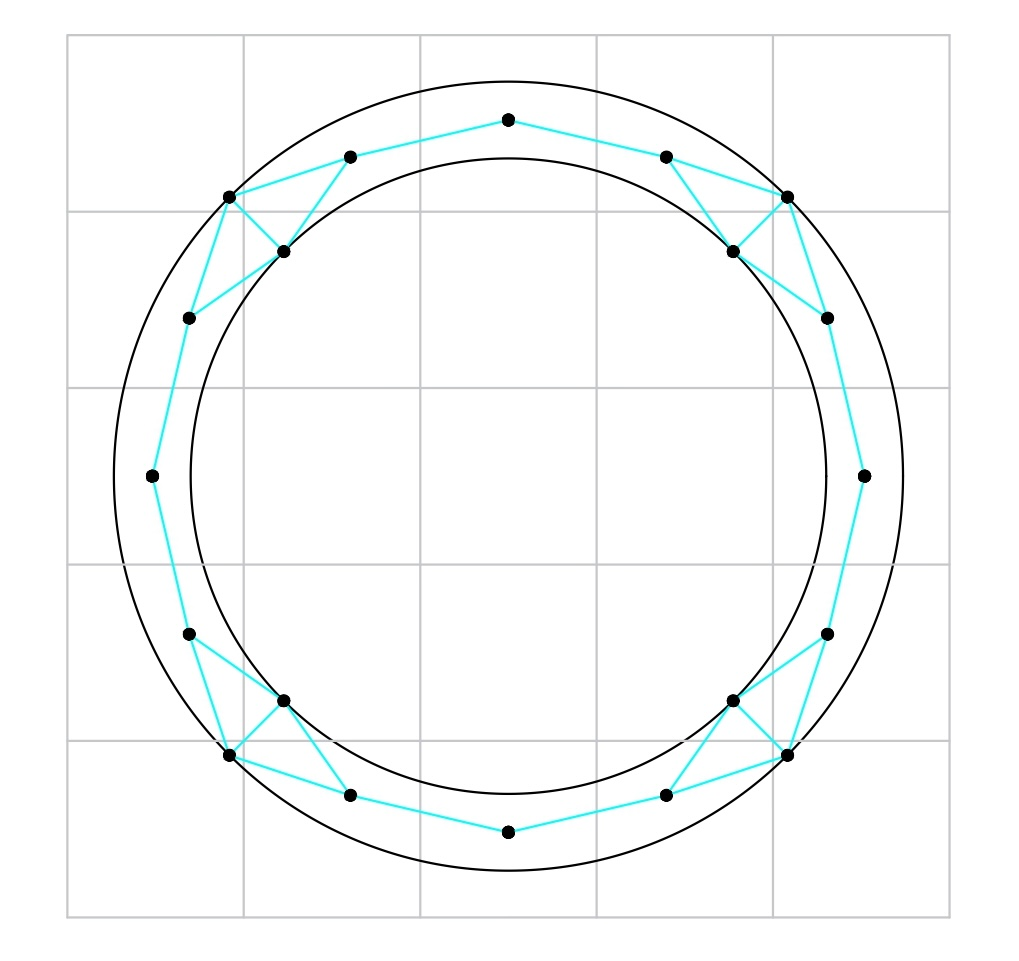
\includegraphics[width=0.52\textwidth]{Figures/DC-manifold-example.jpg}
    \decoRule
    \caption{Visualization of the Dual Contouring algorithm's limitation permits only a single vertex per cell.}
    \label{fig:DC-limitation-ch6}
\end{figure}
As illustrated in Fig. \ref{fig:DC-limitation-ch6}, the object is represented by a very thin ring in black. The QEF point is denoted by the black vertex. The cyan color highlights the surface generated using the Dual Contouring algorithm. Due to the algorithm's limitation of allowing only one vertex per cell, the ring appears infinitely thin. This representation also results in degenerated triangles, which can be observed in the cyan surface.

\subsubsection{Dual Marching Cubes} 
The Dual Marching Cubes algorithm excelled in representing thin-walled structures and intricate thin features. In Figure \ref{fig:DMC-dual-grid-ex-ch6}, a two-dimensional example is presented to elucidate the Dual Marching Cubes algorithm's workings with thin features. The primal grid, foundational to the process, is depicted in light grey. The QEF points, integral to the algorithm, are distinctly marked as black vertices. By connecting these QEF points, we form the dual grid, which is emphasized in contrasting red. The original object, a thin ring, is outlined in black. When the DMC algorithm is applied, the resultant surface, shown in cyan, emerges. Due to the mesh's granularity, the resultant surface is slightly imperfect curvature.

\begin{figure}[H]
\centering
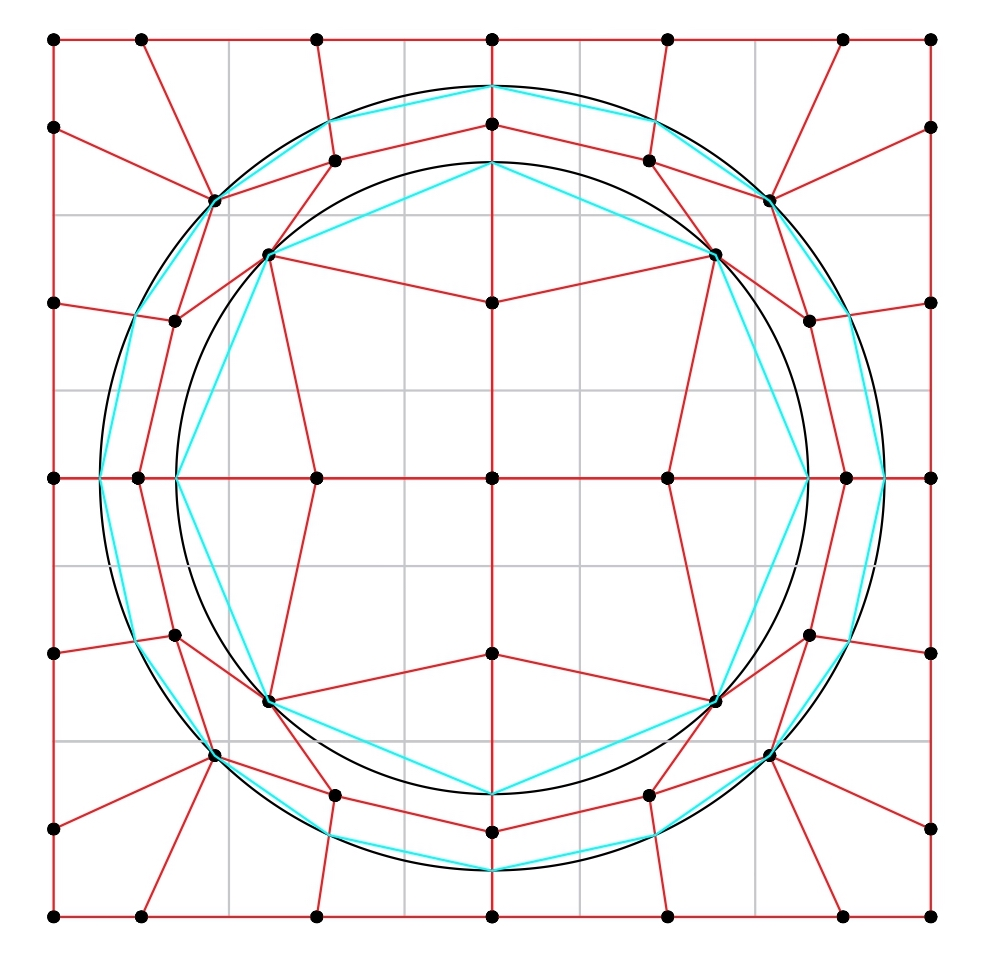
\includegraphics[width=0.5\textwidth]{Figures/DMC-dual-grid.jpg}
\decoRule
\caption{2D visualization of the Dual Marching Cubes Algorithm on a thin ring}
\label{fig:DMC-dual-grid-ex-ch6}
\end{figure}

\subsection{Advantages and Limitations in Practice}

In practical applications, the advantages and limitations of both algorithms became evident. The DC algorithm's ability to preserve sharp features was evident in datasets with geometric shapes, while its limitations (Fig. \ref{fig:DC-analysis-thin-features}), such as the inability to generate thin features, were pronounced in datasets with thin structures.

\begin{figure}[H]
    \centering
    \begin{subfigure}{0.5\textwidth}
        \centering
        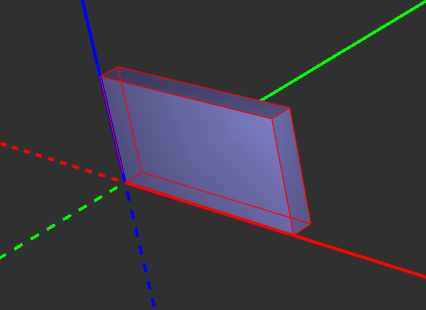
\includegraphics[height=0.7\textwidth, width=0.9\linewidth]{Figures/Thin-brick.png}
    \end{subfigure}%
    \begin{subfigure}{0.5\textwidth}
        \centering
        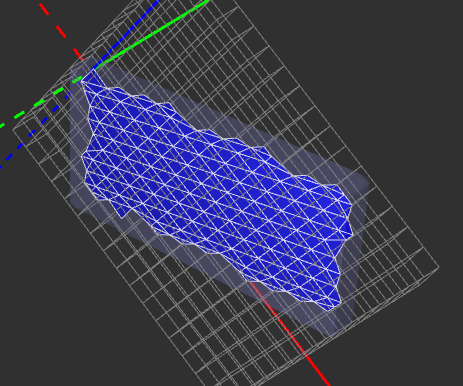
\includegraphics[height=0.7\textwidth, width=0.9\linewidth]{Figures/DC-thin-brick-mesh.png}
    \end{subfigure}
    \decoRule
    \caption{Illustration of the DC algorithm's challenges in handling objects with dimensions smaller than the cell width.}
    \label{fig:DC-analysis-thin-features}
\end{figure}

\noindent The DMC algorithm's strength in representing thin-walled structures was evident in complex datasets (Fig. \ref{fig:DC-DMC-thin-feature}), such as the rocket and room models. However, its computational intensity was a limitation in scenarios requiring real-time mesh generation.

\begin{figure}[H]
    \centering
    \begin{subfigure}{0.5\textwidth}
        \centering
        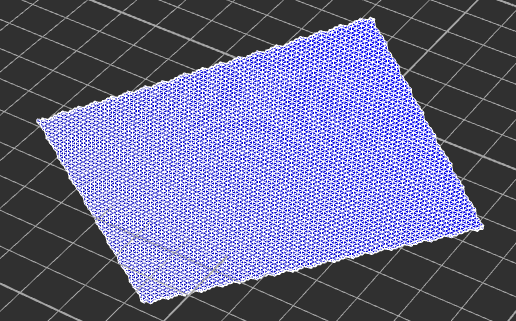
\includegraphics[height=0.7\textwidth, width=0.9\linewidth]{Figures/DC-thin-brick-new.png}
    \end{subfigure}%
    \begin{subfigure}{0.5\textwidth}
        \centering
        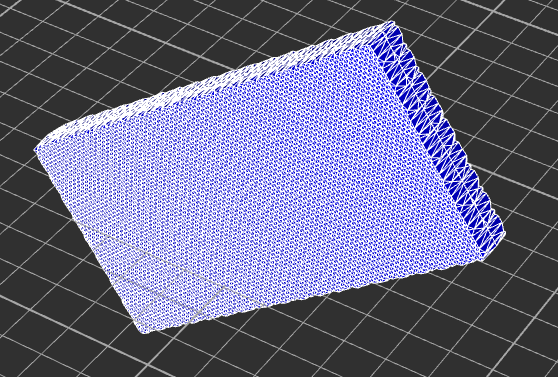
\includegraphics[height=0.7\textwidth, width=0.9\linewidth]{Figures/DMC-thin-brick.png}
    \end{subfigure}
    \decoRule
    \caption{Comparison between DC and DMC algorithms: While DC (left) struggles with thin features, DMC (right) effectively reproduces them.}
    \label{fig:DC-DMC-thin-feature}
\end{figure}

\section{Discussion}

The Dual Contouring and Dual Marching Cubes algorithms offer advanced techniques for isosurface extraction, each with strengths and limitations. The DC algorithm's ability to preserve sharp features makes it suitable for datasets where these features are crucial. However, its computational intensity and memory consumption might be limiting factors for large datasets or real-time applications. The DMC algorithm's strength lies in its ability to represent thin-walled structures. This makes it suitable for applications where the thickness or fineness of structures is a critical factor. However, its computational demand and complexity of implementation might pose challenges in specific scenarios.

In conclusion, the choice between DC and DMC depends on the application's specific requirements. For applications requiring sharp feature preservation, DC might be the preferred choice. For applications focusing on thin structures, DMC might be more suitable.
\chapter{Conclusion and Future Work} \label{Chapter7}

The primary objective of this thesis was to delve deep into the intricacies of isosurface extraction, with a particular focus on the Dual Contouring and Dual Marching Cubes algorithms. Through a comprehensive exploration, the thesis aimed to understand the strengths, limitations, and practical applications of these algorithms and how they can be optimized for various scenarios.

\section{Conclusion}

This thesis began with a comprehensive introduction, framing the problem, delineating the scope, and setting the research objectives. Fundamental concepts are pivotal to understanding isosurface extraction, including the intricacies of Hermite data and the challenges of conformal meshing, were elaborated upon. A thorough literature review followed, comparing various algorithms from the foundational Marching Squares to the intricate Dual Marching Cubes.

The integration of ray tracing was explored, focusing on the Intel Embree API and its role in mesh data structures. The Quadratic Error Function, facilitated by the Eigen Library, was dissected, leading to an equation simplification and a discussion on its minimization challenges. The thesis culminated in a detailed implementation of the Dual Contouring and Dual Marching Cubes algorithms. It was accompanied by a discussion of the results, emphasizing the quality of the generated meshes and their visual fidelity.

The exploration underscored the unique strengths and challenges of both DC and DMC algorithms. While DC shines in preserving sharp features, DMC, building on the strengths of previous algorithms, efficiently represents thin structures with fewer polygons. In essence, both algorithms offer valuable tools in the toolbox of isosurface extraction. The choice between them hinges on the specific requirements and constraints of the application at hand.

However, it's essential to note that the current implementation is far from perfect. The nested loop iterations could be optimized further, and the data structures used can be improved. Transitioning from a 3D nested data structure to a single-dimensional array format with efficient indexing could enhance performance and memory usage. Additionally, the current QEF implementation occasionally produces points outside the desired cell, leading to a patchwork solution of clamping these points to the boundary. This approach, while functional, is not ideal. Furthermore, the algorithm's performance with nested surfaces remains untested due to time constraints.

\section{Future Work}

The exploration of the DC and DMC algorithms has opened up a plethora of avenues for future research and development:

\begin{itemize}
    \item \textbf{Data Structure Optimization:} As discussed in Section \ref{Data-Structure-Optimization}, there's potential for significant optimization in the data structure used to represent the grid. Transitioning from the current 3D nested vector structure to a more efficient representation, such as a single-dimensional array, can offer performance benefits. For a detailed discussion and proposed solutions, refer to Section \ref{Data-Structure-Optimization}.

    \item \textbf{Improved QEF Implementation:} Addressing the current limitations of the QEF implementation, especially the issue of points lying outside the desired cell, is crucial. A more robust solution is needed than merely clamping the points to the boundary.

    \item \textbf{Adaptive Grids:} Future research could delve into adaptive grids, such as octree, that refine in regions of interest. This could lead to more efficient representations and reduced computational demands.
    
    \item \textbf{Optimization Techniques:} There is room for optimization, especially regarding computational efficiency. Exploring parallel processing or harnessing the power of GPUs could significantly reduce the computational time.

    \item \textbf{Real-time Applications:} Adapting these algorithms for real-time scenarios, such as gaming or interactive simulations, is a challenging yet rewarding avenue. This would involve optimizing the algorithms to work within the constraints of real-time rendering.
    
    \item \textbf{Machine Learning Integration:} Integrating machine learning techniques to predict optimal vertex placements or to guide the isosurface extraction process could be a promising direction.
\end{itemize}

\noindent In conclusion, exploring the Dual Contouring and Dual Marching Cubes algorithms has been thorough and insightful. The world of isosurface extraction is vast, and the horizon is dotted with opportunities for innovation, optimization, and novel applications. The journey has just begun.


%----------------------------------------------------------------------------------------
%	THESIS CONTENT - APPENDICES
%----------------------------------------------------------------------------------------

\appendix % Cue to tell LaTeX that the following "chapters" are Appendices

% Include the appendices of the thesis as separate files from the Appendices folder
% Uncomment the lines as you write the Appendices

% Appendix A

% \chapter{Frequently Asked Questions} % Main appendix title

% \label{AppendixA} % For referencing this appendix elsewhere, use \ref{AppendixA}

% \section{How do I change the colors of links?}

% The color of links can be changed to your liking using:

% {\small\verb!\hypersetup{urlcolor=red}!}, or

% {\small\verb!\hypersetup{citecolor=green}!}, or

% {\small\verb!\hypersetup{allcolor=blue}!}.

% \noindent If you want to completely hide the links, you can use:

% {\small\verb!\hypersetup{allcolors=.}!}, or even better: 

% {\small\verb!\hypersetup{hidelinks}!}.

% \noindent If you want to have obvious links in the PDF but not the printed text, use:

% {\small\verb!\hypersetup{colorlinks=false}!}.

%\include{Appendices/AppendixB}
%\include{Appendices/AppendixC}

%----------------------------------------------------------------------------------------
%	BIBLIOGRAPHY
%----------------------------------------------------------------------------------------
\printbibliography[heading=bibintoc]

%----------------------------------------------------------------------------------------

\end{document}  
